\documentclass[11pt,a4paper,twoside]{article}

\usepackage[english]{babel}
\usepackage[T1]{fontenc}
\usepackage[utf8]{inputenc}
\usepackage{blindtext}
\usepackage{pdfpages}
\usepackage{multirow}
\usepackage{rotating}
\usepackage{booktabs, array, ragged2e}
\newcolumntype{P}[1]{>{\RaggedRight\arraybackslash}p{#1}}
\newcommand{\tabitem}{\textbullet~~}
\usepackage{tabularx}
\usepackage{enumitem}
\usepackage{caption}
\usepackage{eurosym}
\usepackage{arydshln}


\usepackage[
    plainpages=false,
    bookmarks=true,
    bookmarksopen=true,
    colorlinks=false
]{hyperref}

\usepackage{apacite}

\usepackage{etoolbox}
\makeatletter
\patchcmd{\APACjournalVolNumPages}%
    {\unskip, \Bem{#2}}%
    {\unskip, #2}{}{}
\makeatother


\usepackage[super]{nth}

%% IMAGE PACKAGE
\usepackage{graphicx}

%% PACKAGE FOR THE BACKGROUNDPIC
\usepackage{eso-pic}

%% PACKAGE FOR THE HEADERS AND FOOTERS
\usepackage{fancyhdr}

%% PACKAGE FOR THE BIBLIOGRAPHY
%\usepackage[
%    backend=biber,
%    style=apa,
%    citestyle=apa
%]{biblatex}
%\bibliography{MyReferences}


\interfootnotelinepenalty=10000

\newcommand\BackgroundPic{%
\put(0,0){%
\parbox[b][\paperheight]{\paperwidth}{%
\vfill
\centering

\includegraphics[width=\paperwidth,height=\paperheight,keepaspectratio]{template/background.pdf}%
\vfill
}}}

\fancyhf{}% Clear all headers/footers
%\renewcommand{\headrulewidth}{0pt}% No header rule
%\renewcommand{\footrulewidth}{0pt}% No footer rule
%\fancyfoot[L]{\hspace*{-16mm}
\includegraphics[scale=0.3]{template/logoDepartment.pdf}}
\fancyhead[LE,RO,LO,RE]{}
\fancyfoot[CE,CO,RE,LO]{}
\fancyfoot[LE,RO]{\Roman{page}}
\renewcommand{\headrulewidth}{0pt}
\setlength{\headheight}{13.6pt} % behebt headheight Warning

% Korrektes Format für Nummerierung von Abbildungen (figure) und
% Tabellen (table): <Kapitelnummer>.<Abbildungsnummer>
\makeatletter
\@addtoreset{figure}{section}
\renewcommand{\thefigure}{\thesection.\arabic{figure}}
\@addtoreset{table}{section}
\renewcommand{\thetable}{\thesection.\arabic{table}}
\makeatother

\sloppy % Damit LaTeX nicht so viel über "overfull hbox" u.Ä. meckert

% Ränder
\addtolength{\topmargin}{-16mm}
\setlength{\oddsidemargin}{25mm}
\setlength{\evensidemargin}{35mm}
\addtolength{\oddsidemargin}{-1in}
\addtolength{\evensidemargin}{-1in}
\setlength{\textwidth}{15cm}
\addtolength{\textheight}{34mm}

%______________________________________________________________________
\begin{document}

\pagestyle{empty} % Vorerst keine Seitenzahlen
\pagenumbering{alph} % Unsichtbare alphabetische Nummerierung

%__Declaration begin__________________________________________________

\includepdf[pages={1}]{template/scan-of-declaration-of-authorship.pdf}
\cleardoublepage
%__Declaration end____________________________________________________

%__Cover Page begin___________________________________________________
\AddToShipoutPicture*{\BackgroundPic}
%\thispagestyle{fancy}

{\vspace{2cm}~}
{\vspace{4cm}}

%% SELECT BACHELOR OR MASTER THESIS
{\noindent\Large Bachelor Thesis}


\vspace{1cm}

%% WRITE THE TITLE OF YOUR WORK
{\noindent\Huge\textbf{Careers of Project Professionals – \\[.2cm]
{\huge A project type and industry perspective}}}

\bigskip

%% WRITE YOUR NAME, date of birth, Student ID
{\noindent\huge Matthias Gutheil}

%% WRITE YOUR date of birth, Student ID
\smallskip
{\noindent\small Date of Birth: 28.02.1995 \\}
{\noindent\small Student ID: h1600738}

\smallskip
{\vspace{2cm}}
{\noindent\Large {\bf Subject Area:} Project Management}

\smallskip

%% WRITE YOUR Studienkennzahl
{\noindent\Large {\bf Studienkennzahl:} J 033 561}

\smallskip

%% WRITE THE NAME OF YOUR SUPERVISOR
{\noindent\Large {\bf Supervisor:} a.o.Univ.Prof. Dr. Martina Huemann}

\smallskip

%% WRITE THE DATE OF SUBMISSION
{\noindent\Large {\bf Date of Submission:} 31. August 2018}

\bigskip\bigskip\bigskip

{\em\noindent Project Management Group, Department of Strategy and Innovation, Vienna University of
Economics and Business, Welthandelsplatz 1, 1020 Vienna, Austria
}
\bigskip\bigskip\bigskip\bigskip

\begin{figure}[hbt]
 % \centering
  
\includegraphics[width=.35\columnwidth]{figures/pmg_logo.jpg}
  \label{fig:pmg_logo}
\end{figure}

\pagebreak
%__Cover Page end___________________________________________________

\cleardoublepage
\begin{abstract}
\blindtext
\end{abstract}

%______________________________________________________________________
\cleardoublepage
\pagestyle{fancy}
\pagenumbering{roman} % Römische Seitenzahlen

\tableofcontents
\addtocontents{toc}{\protect\setcounter{tocdepth}{3}}
%______________________________________________________________________

\clearpage
%\addcontentsline{toc}{section}{\listfigurename}
\listoffigures

\clearpage
%\addcontentsline{toc}{section}{\listtablename}
\listoftables

%______________________________________________________________________
\cleardoublepage
\pagenumbering{arabic}
\setcounter{page}{1}
% Geändertes Format für Seitenränder, arabische Seitenzahlen
\fancyhead[LE,RO]{\rightmark}
\fancyhead[LO,RE]{\leftmark}
\fancyfoot[LE,RO]{\thepage}


\cleardoublepage

\section{Introduction}
\label{sec:Introduction}
For quite a while now, project-based jobs and organisations are on the rise. This development is fuelled by the fact that many companies are struggling to cope with the accelerating changes triggered by globalisation and its byproduct digitisation, which requires them to be more agile and flexible. 
... [MISSING]

\subsection{Rational and motivation}
This thesis is part of the \textit{Project Management institute (PMI)} funded research project 'careers@projects', which is collaboratively conducted by a team of researchers from the \textit{Department of Strategy and Innovation} of the \textit{Vienna University of Economics and Business (WU)} and from the \textit{Human Resource Management and Employment Relations Faculty} of the \textit{University College Dublin (UCD)}. Its comprehensive objectives are to research the career making activities of project professionals on projects, to analyse challenges and opportunities to acquire career resources on projects and to ultimately describe implications and make recommendations for project professionals and companies interested in improving understanding of careers on projects. The methodology used by the researchers to achieve these goals is a knowledge co-creation process with project professionals, consisting of qualitative in-depth interviews and focus group workshops. As a research assistant the author of this thesis was involved in all activities of the research project, during its pilot phase. Therefore, he had the opportunity to not only gain an in-depth understanding of the subject matter, but also to evaluate a first version of his working framework in a focus group workshop with project professionals.

\subsection{Objectives and research questions}

\noindent {\bf Objectives}\\[.1cm]
Based on the before described exploratory context of this thesis, the  main objective is to develop a framework, which can be used to analyse the careers of project professionals regarding: at what stage, in what matter and why they change between project types or industries in their career. Moreover, the so far gathered data shall be used to draw conclusions and to propose adjustments and potential fields for future research to analyse. Lastly, adjustments to the preexisting questionnaire are to be made, in order to provide the required data for the working model. Above all, this bachelor thesis' goal is to contribute to the higher goal of the research project, which is to gain a deeper understanding of the careers of project professionals.\\

\noindent {\bf Research questions}\\ [.1cm]
In the context of the complex research field project management and the wide range of the overarching research project 'careers in projects' it was important to narrow down the scope of this work. Therefore, and also in respect to the research-objective, the research questions are defined as follows: 
\begin{itemize}[itemsep=0.05cm]
    \item What are patterns in the careers of project professionals after 5 | 10 | 15 | 20 years?
    \item How often do project professionals change project types and industries?
    \item What are patterns behind these changes?
\end{itemize}
\clearpage

\subsection{Research methodology}
The research methodology of this thesis and the overarching research project is based on the 4D model introduced by \citeA{maylor17}.
It consists of four steps, being \textit{D1 - Defining}, \textit{D2 - Designing}, \textit{D3 - Doing} and \textit{D4 - Describing}, which are aimed at providing guidance and structure to students conducting business and management research. In the following the research methodology of this thesis is explained using the before named, four steps of the 4D model. \\

\subsubsection{D1 - Defining}
The first step, Defining, deals with understanding academic research itself, generating and clarifying ideas and using sources of information. Based on their model, \citeA[p. 6]{maylor17} define research as 
\begin{quote}
"A systemic process that includes defining, designing, doing and describing an investigation into a particular problem."
\end{quote}
The general problem from the business and management field that is dealt with in the scope of this the research project, careers@projects, are the career developments of project professionals. The particular problem, which is derived from this general problem and that is investigated in this thesis, consists in patterns in careers of project professionals respectively project contents and industries. With reference to the stage of defining, the main difficulties faced are to differentiate the group of project professionals from other professionals, to narrow the investigative vision to the problems related to project management and to accumulate a solid theoretical basis for the final framework. Therefore, in order to deal with this complexity, an extensive literature review in relation to all relevant fields was conducted, including key words like \textit{project professionals}, \textit{project types}, \textit{project industries}, \textit{project personnel}, \textit{project classification}, \textit{project categorisation}, etc.. \\
At this point, apart from identifying these directly to the thesis related problems, the overarching research project's contexts should be looked at, in order to gain a better understanding of important correlating fields and issues. The research project is based on the concept of boundaryless careers, which captures the phenomenon of recent years that careers become more flexible, dynamic and the shift away from the organisation taking responsibility of its employees career, towards one by himself/herself having to take responsibility of one's own career \cite{inkson09}. This development challenges not only, but especially project-based organisations to develop new career paths and options in order to maintain skilled personnel. Therefore, this research is not only relevant from a academic viewpoints, but also from a practical one. So as to be able to develop such bespoke measures, organisations need to understand what underlying patterns influence and shape the careers of project professionals. Finding these patterns and explaining them is the purpose of the research project.\\

\subsubsection{D2 - Designing}
In the second part, Designing, the research approach itself is dealt with, as well as the means of conducting qualitative, quantitative and case study research \cite{maylor17}. \\
%DEFINITION OF RESEARCH APPROACH AND THE THREE APPROACHES\\
The research approach selected for this research project is qualitative as defined by \citeA{yin15}. It was selected due to the socio-scientific perspective taken in this study and implemented by the repeated execution of the following research methods with 60 project professionals: 
\begin{itemize}[itemsep=0.05cm]
    \item Indirect data collection: Curriculum vitae (CV)
    \item Observation: Systematic constellation and ground anchor
    \item Interview/Discussion: In-depth interviews
    \item Participating: Focus group workshops
\end{itemize}
The data collection methods incorporate increasing levels of personal involvement with the subject and thereby ensure a significant and sufficient database \cite{maylor17}. At this point should be noted that of the 60 interviews conducted the data of 20 was available in July 2018 in order to test the developed working framework. The other 40 interviews were conducted, but the interviews were not transcribed and therefore could not be analysed.\\
In the following each of the applied research methods will be explained in depth.\\

\noindent {\textit{Curriculum Vitae}}\\[.1cm]
As a result of the research project being in its pilot phase, the request of a CV from each candidate had, on the one hand, the purposes to gain basic information, like birth date, nationality, etc.,  from the interviewee. Furthermore, it was aimed at obtaining data regarding the roles conducted in each company and the projects performed. However, in the course of the performance of the interviews, a restriction regarding this data collection method was discovered, which constitutes in the fact that many project professionals who have worked for a long period of time in the same company have not had the need to make up a CV, as they did not apply for any position. Therefore, the necessity for a questionnaire  was identified. Developing it, considering also the data needed for the developed framework, is one of the goals of this thesis.\\ 

\noindent {\textit{Systematic constellation and ground anchor}}\\[.1cm]
The interviews were enriched with a ground anchor method, a variation of the systematic constellation method \cite{huemann16}, in which the interviewee visualises his careers and other important events, resources or projects by placing differently coloured and/or shaped cards on the ground. There were no rules, nor restrictions in regards to the degree of detail, use of colours, etc.. The goal was to help the candidate visualising and reflecting on his career during the interview, as he walked through his constellation during the interview. Moreover, the forms created were photographed to be used as data themselves in future phases of the research project. \\

\noindent {\textit{In-depth interviews}}\\[.1cm]
The interview was conducted as a one-on-one, semi-structured, personal interview \cite{maylor17}. Furthermore, it was split in three parts. In the first part, the interviewee walked through his created formation, describing for each step his/her role, whether it had been a project, the duration, the complexity and the impact on his/her career and in general if there had been a reason behind the selection of colours and shapes. In the second part, the project professional once again steps on all stations, this time explaining the competences gained or lessons drawn from each position/project. Finally, the interviewee is asked to reflect on his career as whole. The majority of the interviews were conducted in German, which required additionally to the transcription, the translation of the transcripts. Due to the number and length of each of the interviews, the translations were made using an advanced, machine-learning based online service.\\


\noindent {\textit{Focus group workshops}}\\[.1cm]
The focus groups conducted by the research team met all defined characteristics that should be inherent to this type of workshop. These criteria are "(1) a small group of people, who (2) possess certain characteristics, (3) provide qualitative data (4) in a focused discussion (5) to help understand the topic of interest."\cite{krueger14}
As of July 2018, two focus groups were conducted in the scope of the research project. The first one was in November 2017 in Munich, at an early stage of the exploratory study. It was aimed at collecting information on hindering factors (obstacles) and supporting factors for project careers in the context of infrastructure projects. It was attended by 11 members of the NETLIPSE network. The second workshop took place in May 2018 in Vienna and was targeted at evaluating and receiving feedback on first models of the final frameworks, one of them being the one developed in this thesis. Moreover, first results were presented to the 7 participants. \\

\subsubsection{D3 - Doing}
The third part, Doing, focuses on considerations to be taken in doing research, the description and analysis of the using statistical tests and the interpreting of words and actions \cite{maylor17}.\\
One crucial aspect regarding this part is, gaining access to people and organisations, which are willing to participate in the study. Since participants with specific requirements, respectively the project professional criteria, were needed for the study, one of the main means was leveraging on contacts of the researchers involved, like the connection to Austria's project management association \textit{PMA} or people known through prior research projects. In the first part of the project, first and foremost warm contacts, which are people with whom a preexisting connection exists \cite{maylor17}, were invited to participate. In later stages also a connection to cold contacts, which are people unknown to you and with whom you have nothing in common \cite{maylor17}, was established. As a result, a total of 60 interviews were conducted, of which the qualitative data of 20 are the basis to this thesis. Out of these 20, 17 are male. Moreover, the median age is 49 years, the median professional experience amounts to 22,5 years and the majority (65 per cent) has an IT background. Apart from this short introduction, the sample group will be introduced in detail in the \nth{4} chapter. The key challenges regarding the analysis of qualitative data like this are according to \citeA{maylor17}:
\begin{itemize}[itemsep=0.05cm]
    \item The data is not process nor transformed
    \item The data takes many forms
    \item The data is not standardised
    \item The data is voluminous 
\end{itemize}
Furthermore, it is crucial to ensure that the data is traceable, reliable and complete. Consequently, the main challenge of qualitative research is to derive the most important information from all data available and to insert it into a form (e.g. a matrix), which enables the research to analyse it \cite{maylor17}.\\
Accordingly,  so as to meet the challenges and to achieve a correspondence with other qualitative requirements, a analysis matrix was developed. The approach to the development of the matrix was both structured and unstructured, in the sense that the research instruction provided a formal structure for the matrix, which was extended and adapted based on the information obtained from the data. The matrix was made using Microsoft Exel. It is split into two parts, each displayed in their own spreadsheet. The first one contains an analysis of the basic data of each interviewee, including interview ID, age, gender, current industry, current company, type of employment, role and country of employment. The second one analyses the career of each project professional, starting with the first named full-time profession in the CV. From there an analysis of the indicators is made every 5 years, respectively after 5 | 10 | 15 | 20 | 25 years. The attributes analysed in each time span and for each interviewee are:
\begin{itemize}[itemsep=0.05cm]
    \item Total number of projects conducted
%    \item Average project scope (\euro)
    \item Number of different project industries worked in
    \item Name(s) of the industry(/ies) worked in (from a default list)
    \item Number of different project contents worked in
    \item Name(s) of the project content(s) worked in (from a default list)
    \item Number of company changes
\end{itemize}
The names of the project industries/contents are the only indicators that were answered in free text. For the analysis they were grouped, based on preexisting basic research, which is presented in depth in the following chapter. As the numeric data, such as the number of projects, is also in some cases deduced from non-numeric data, it relies also on the definitions and concepts presented in chapter \ref{sec:LiteratureRev}. Apart from these aspects, it has to be pointed out, that the necessity for some of the indicators was discovered during the analysis process. Furthermore, as the in-depth interviews were conducted in an semi-structured way and as a result not for all data sets is information available. Moreover, the analysis was restricted by the fact that some interviewees could not share all required information, due to their company's non-disclosure policy or they simply just did not know. Above all, a restricting factor was the general aspect that the interviews were not conducted specifically for this thesis, and therefore they are not able to cover all aspects of the for the answering of the research question required data.

\subsubsection{D4 - Describing}
The forth and last part, Describing, covers the topics making sense of the findings and presenting, reflecting and learning from the research conducted \cite{maylor17}. \\
In order to provide the reader with a guiding thread throughout the entire thesis, before the start of the actual writing process, a logically structured table of contents was developed and visualised, listing important aspects that need to be covered within each of the structure's points. Moreover, the thesis introduces the reader to the topic and the research in a logical manner, orientating on the generic project report structure proposed by \citeA{maylor17}.

\subsection{Summarised overview of chapters}
The first chapter provides an introduction to the thesis, by firstly elaborating the motivation and rational before describing its objectives and the applied research methodology. In the following chapter the foundations are laid in the means of a literature review dealing with relevant terms and concepts. In the third chapter the actual working framework will be explained, alongside with the considerations taken during the development process. In the forth chapter, after a introduction to the conducted study itself, the study's results are presented and subsequently discussed in the fifth chapter. Lastly, in the final chapter, conclusions are drawn from the findings and recommendations proposed for future research.

\cleardoublepage

\section{Literature review}
\label{sec:LiteratureRev}

In the following chapter, the important terminology and concepts will be described on the basis of the most relevant and recent literature and the current state of research in the project management field. These elaborations will serve as a common ground for the later presented framework itself, as well as for its discussion. 

%____________________________________________________________________
\subsection{Projects}
In literature an great number of definitions of projects can be found, fitting many contexts and purposes. Therefore, in the following three definitions are presented that should serve as theoretical basis for the understanding of projects in the framework of this thesis.

%__project definition 1
The first definition by \citeA[p. 70]{cleland83}, of which the former was one of the founding members of the Project Management Institute (PMI), specifies projects as "A complex effort to achieve a specific objective within a schedule and budget target, which typically cuts across organisational lines, is unique and  is usually not repetitive within organisation." This definition is relevant in the context of this thesis, since it points out, apart from general aspects like the existence of a schedule or budget as a framework, that most projects are collaborative activities that unite (human) resources from different parts of an organisation to work towards an common goal. This aspect is furthermore important in order to understand the concept of project professionals as well as their careers.

%__project definition 2
Another definition of projects, which originates from an article researching projects as a temporary organisation  by \citeA[p. 7]{Turner03}, defines projects as "A project is a temporary organization to which resources are assigned to undertake a unique, novel and transient endeavour managing the inherent uncertainty and need for integration in order to deliver beneficial objectives of change." The reason behind the selection of this definition is that it points out that many projects in organisations are created in order to cope with the complexity of innovative or unknown undertakings, as well as to test them in a restricted environment. Thereby, the organisation can not only limit the consequences of a potential failure, but also circumvent rigid structures within and facilitate, respectively enable, the exchange of know-how and experience across different departments.

%__project definition 3
\noindent The third and last definition of projects is constituted by the following Table \ref{tab:process}, which uses certain process characteristics to attribute the appropriate organisation type for the fulfilment of different business processes.\\

\begin{table}[!hbt]
\captionsetup{font=small}
\footnotesize
\centering
    \begin{tabular}{| l | c | c | c |}
    \hline
    {\bf Process characteristic} & \multicolumn{3}{ |c| }{{\bf Attribute}} \\
    \hline
    Frequency & often & once & once \\ \hline
    Scope & small-medium & medium-large & large  \\ \hline
    Importance & low & medium-high & high \\ \hline
    Duration & short & short-medium & medium-long \\ \hline
    Resources & few & some & many \\ \hline
    Costs & low-medium & medium-high & high \\ \hline
    Number of organisations & few & several-many & many \\ \hline
    \multicolumn{1}{ c }{} & \multicolumn{1}{ c }{$\downarrow$} & \multicolumn{1}{ c }{$\downarrow$} & \multicolumn{1}{ c }{$\downarrow$} \\ \hline
    Type of organisation & Permanent organisation & Project & Program \\ \hline 
    \end{tabular}
    \caption[Adequate organisations for different process types]{Adequate organisations for different process types. Adapted from Human Resource Management in the Project-Oriented Organization: Towards a Viable System for Project Personnel (p. 44), by Huemann, M., 2015, Aldershot: Gower.}
\label{tab:process}
\end{table}

This concept was chosen over other very commonly used concepts like the ones showing the differences between project, program and portfolio management (see Appendix A on page \pageref{tab:pmbok}), since it points out process characteristics of not only in temporary constructs like projects or programs, but also in the permanent organisation. Therefore, it helps respectively the interviews and data gathered to interpret which of the described processes or tasks taken out by the interviewees are actually project-processes and which are not.\\

Considering the three named definitions of projects there are five key aspects that can be derived and that are relevant to the understanding of further evaluations in this thesis. These key aspects are:
\begin{itemize}[noitemsep]
    \item projects are temporary
    \item projects are complex
    \item projects are made up by personnel across lines
    \item projects have a defined objective
    \item projects are restricted by a budget and a schedule
\end{itemize}

\subsection{Project categorisations}
Following the definition of projects themselves, in the next step, various ways of categorising projects will be introduced and out of these two, which are the categorisation by content and by industries, will be evaluated in depth as they form the basis of the final working model. The reason for the selection of these two categorizations out of the rest is explained in the next Chapter in Considerations. 

Projects can be categorised in many ways. The reasons behind wanting to categorise projects in the first place are according to \citeA[p. ix]{crawford05}: "[...] to identify the level of approval they require, the competencies and training needs of project management personnel, the methods and techniques that will be appropriate to apply to their management, which budget will fund them, and their alignment with organizational strategy." In comparison, \citeA{archibald04} lists as key benefits that would result from a global project categorisation system:
\begin{itemize}[noitemsep]
    \item Selection and development of the best project life cycle (or life span) models 
    \item Identification and application of best practices for 
        \begin{itemize}
            \item Project selection and prioritization
            \item Planning, executing and controlling methods and templates
            \item Risk management methods
            \item Governance policies and procedures
            \item Development of specialized software applications
        \end{itemize}
    \item Building of specialized bodies of knowledge
    \item Selection and training of project managers and project management specialists 
    \item Focusing and improving PM education and training
    \item More effective individual PM certification and career planning
    \item More focused research efforts 
\end{itemize}

A very basic way of classifying projects and thereby identifying certain project types, is the classification by if the project goals and the methods to achieve them are well-defined. \citeA{turner93} developed using this approach the \textit{Goals-and-methods matrix} (see figure \ref{fig:gmmat} on page \pageref{fig:gmmat}), which defines four project types and provides for each a chance of success/failure for each. 


\begin{figure}[!hbt]
    \captionsetup{font=small}
  \centering
  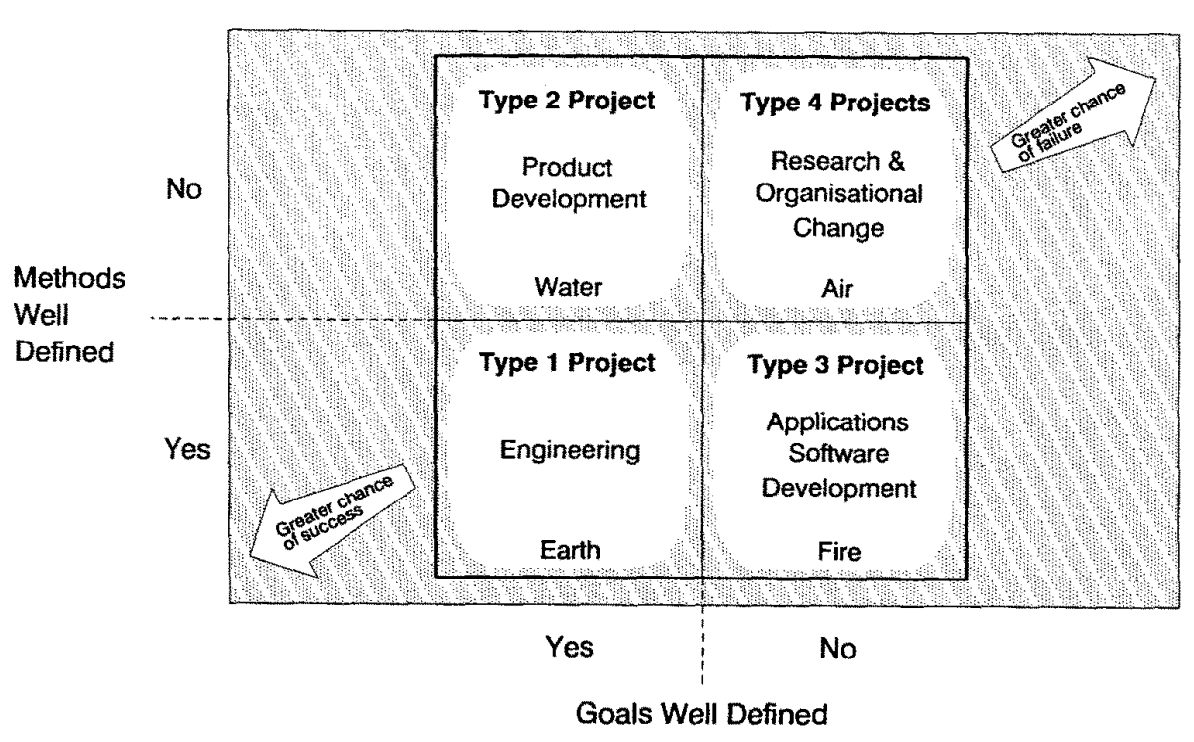
\includegraphics[width=.6\columnwidth]{figures/goal_mathods-matrix.png}
  \caption[Goals-and-methods matrix]{Goals-and-methods matrix. Reprinted from “Goals-and-methods matrix: coping with projects with ill defined goals and/or methods of achieving them,” by Turner, J.R. and Cochrane, R.A., 1993, Journal Title,International Journal of Project Management, 11(2), pp.93–102.}
  \label{fig:gmmat}
\end{figure}


Before providing an example of an actual categorisation system, the very basis of such systems should be looked at, which are the attributes that are relevant in the context of grouping projects. Many categorisation approaches that can be found in recent literature \cite<e.g., >{huemann15,turner10} are based on an empirical study by \citeA{crawford05}, which identifies 37 different attributes of categorisation that are used in project-oriented organisations. The identified attributes of this basic research, which are defined  by the authors as "the underlying characteristic that is being used to categorize projects" \cite[p. 28]{crawford05}, can be seen in Appendix B on page~\pageref{tab:cate1}. Out of the 37 attributes identified, table \ref{tab:cate2} on page~\pageref{tab:cate2} displays the ten most commonly used and the most important ones and identifies minor variations. The in the beginning of this section named motivation behind the categorisation is further supported by the result of the assessment of the organisational purposes in the scope of the research project, which ascertained as the three most named purposes 'resourcing and planning', 'matching methods to projects' and 'risk assessment' \cite{crawford05}.\\


\begin{table}[!htb]
\captionsetup{font=small}
\centering
\footnotesize
    \begin{tabular}{| l | l |}
    \hline
    {\bf Most Commonly Used Attributes} & {\bf Most Important Attributes} \\
    \hline
    1. Application area & 1. Organisational benefit \\
    2. Nature of work & 2. Cost \\
    3. Client/customer & 3. Client/customer \\
    4. Complexity & 4. Application area \\
    5. Cost & 5. Complexity  \\
    6. Size & 6. Strategic importance \\
    7. Strategic importance & 7. Risk level \\
    8. Risk level & 8. Nature of work \\
    9. Organisational benefit & 9. Resources \\
    10. Deliverables & 10. Size \\
     \hline 
    \end{tabular}
    \caption[Comparison of most common and most important attributes]{Comparison of most common and most important attributes. Adapted from Project Categorization Systems: Aligning Capability with Strategy for Better Results (p. 52), by Crawford, L., Hobbs, B. and Turner, J.R., 2005, Pennsylvania: Project Management Institute.}
\label{tab:cate2}
\end{table}


A practical approach to the categorisation of projects by organisations is constituted by multidimensional or composite systems \cite{crawford06}. Figure \ref{fig:cate}, an example for such a system, visualises the key feature of such systems, which is to combine hierarchical and parallel systems. Hierarchical systems use in the first step one parameter, for example project scope, and then apply different means for each category. Parallel systems, in contrast, make use of composite attributes to group projects. As suggested by the name, composite attributes are composed of a variation of attributes in order to be able to define more sophisticated categorisation attributes. The most common example constitutes \textit{complexity}, which can be described in organisations by using between 2 and 12 attributes. Out of these 'project scope', 'number of cites locations, countries', 'number of functions or skills', 'organisational involvement' and 'clarity of goals/objectives' are the ones organisations use the most \cite{crawford05}. \\


\begin{figure}[!hbt]
    \captionsetup{font=small}
  \centering
  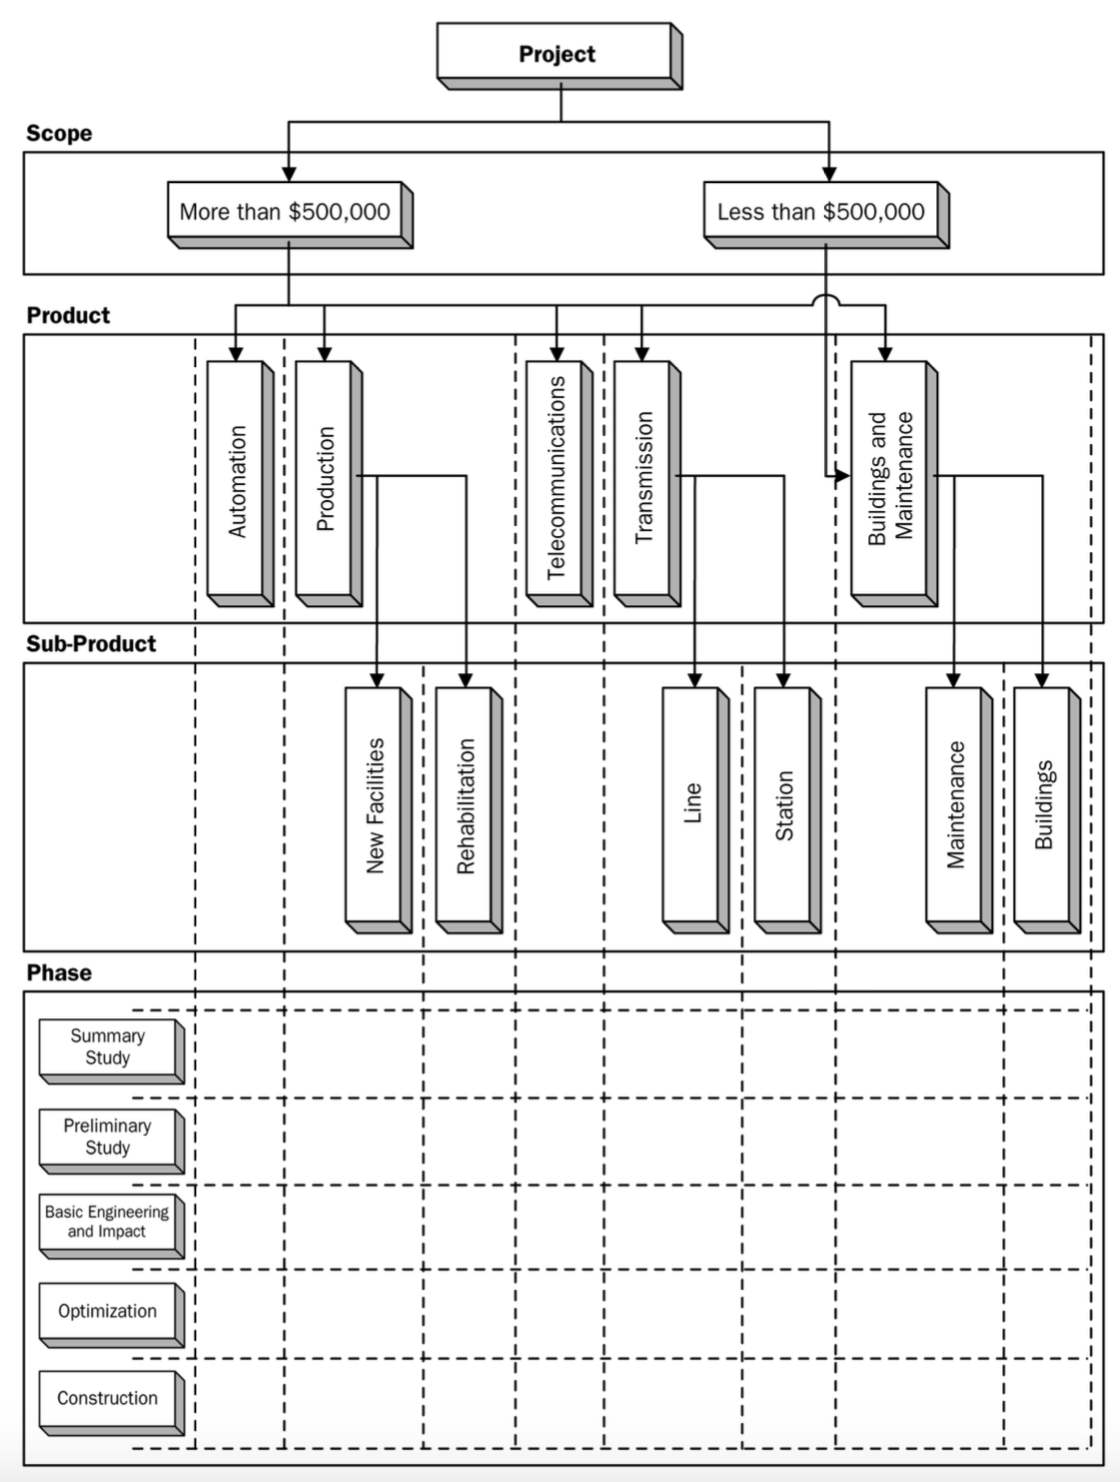
\includegraphics[width=.45\columnwidth]{figures/multidimensional_system.png}
  \caption[A hierarchical categorization with an overlay by phase]{A hierarchical categorization with an overlay by phase. Adapted from Project Categorization Systems: Aligning Capability with Strategy for Better Results (p. 33), by Crawford, L., et al., 2005, Pennsylvania: Project Management Institute.}
  \label{fig:cate}
\end{figure}


%____________________________________________________________________
\subsubsection{By project content}
The categorisation of projects by their content or, as phrased by \citeA{crawford05}  respectively their 'nature of work', is, as can be seen in table \ref{tab:cate2} on page \pageref{tab:cate2}, the \nth{2} most commonly used and the \nth{8} most important attribute. The project's content refers in this context to the very purpose of a project. For example, if a project is started to organise an event, it will incorporate tasks like programming a website, planning the all acts, etc., however, this does not mean it is a planning or an IT project, but an event project. 
A list of possible project contents adapted from \citeA{patzak17} is displayed below. 

\begin{itemize}[noitemsep]
    \item Company formation and acquisition projects
    \item Company participation projects
    \item Marketing projects, event projects
    \item Strategy projects
    \item Acquisition projects, tender projects
    \item Feasibility studies, planning projects
    \item Research projects, product development projects
    \item Organisational development projects
    \item IT projects
    \item Investment projects (construction, plant engineering, etc.)
    \item Maintenance projects, major repairs
\end{itemize}

%introducing also the categorization by archibald04


%____________________________________________________________________
\subsubsection{By project industry}
\label{sec:LiteratureRev:PCategorisation:ByPIndustry}
The application of projects in various industries has increased immensely over the past decades and since 2000 project-based work is being used in all industries and the public sector \cite{morris97, soderlund11}. Even though the categorisation by industry sector is neither ranked among the top ten most commonly used attributes, nor among the most important attributes in the results of the empirical research by \citeA{crawford05} (see table \ref{tab:cate2} on page \pageref{tab:cate2}), it is nevertheless an relevant attribute due to the fact that it is a label inherent to every project. Moreover, there is a significant correlation between industry and technology applied and based on a specific industry there can be drawn inferences about other project aspects such as common markets or project types \cite{huemann15}.
In the project management literature there can be found a variation of classifications for projects by industry-types \cite<e.g.>{wirth96, turner00}. However, since existing industries change or vanish and new industries emerge due to global phenomenons like globalisation or accelerating technological change, a potential list of industry types should be current. An example for such a collection of industries represents the following table \ref{tab:indu} on page \pageref{tab:indu} by \citeA{huemann15}. This list has its origin in the questionnaire of the before-mentioned study by \citeA[p. 148-153]{crawford05} and structures the industries by sectors.

\begin{table}[!htb]
    \captionsetup{font=small}
    \centering
    \small
    \begin{tabular}{ |l|l| }
    \hline
    {\bf Sector} & {\bf Industry} \\
    \hline
    \multirow{6}{*}{Engineering and construction} & Building \\
     & Infrastructure \\
     & Process plant \\
     & Defence \\
     & Aerospace \\
     & Environmental and waste \\ \hline
    \multirow{4}{*}{Information and telecommunications} & E-commerce \\
     & Information technology \\
     & Information systems \\
     & Telecommunications \\ \hline
    \multirow{7}{*}{Services} & Arts, entertainment, broadcasting \\
     & Recreation and sport \\
     & Business and consulting \\
     & Education and training \\
     & Financial services and insurance \\
     & Health and social services \\
     & International development \\ \hline
    \multirow{6}{*}{Industrial} & Automotive \\
     & Electronics \\
     & Manufacturing \\
     & Chemicals and pharmaceuticals \\
     & Food \\
     & Research and development \\
    \hline
    \end{tabular}
    \caption[Projects by industry type]{Projects by industry type. Adopted from Human Resource Management in the Project-Oriented Organization: Towards a Viable System for Project Personnel (p. 48), by Huemann, M., 2015, Aldershot: Gower.}
    \label{tab:indu}
\end{table}

\clearpage
%____________________________________________________________________
\subsection{Project professionals}
There doesn't exist a clear definition of the term project professional (PP) in the literature, since it was created within the scope of the research project 'careers@projects'. Nevertheless, from the perspective of its meaning, there are preexisting terms that can be used as synonyms in order to understand which project management roles are incorporated in the term project professionals.

Such a synonym represents the notion \textit{project personnel}, which is defined by \citeA[p. 76]{huemann15} in the context of the project-oriented organisation as "those human resources who need to draw on project management competency to fulfil their roles [...]". Apart from the general definition, it is important to differentiate project management personnel from the other types of personnel in the project-oriented organisation, management personnel and expert personnel. Management personnel, for instance line managers or department heads, have not only management responsibility, but also personnel authority and live off their management competencies. On the other hand, expert personnel contribute their competencies in order to fulfil their roles, such as functional or technical competencies. Another important differentiating factor of project personnel from other types of personnel in the project-oriented organisation is their contractual situation. According to \citeA{keegan03}, up to 80 per cent of personnel in projects has temporary contracts compared  to only between 20 and 40 per cent of personnel in the project-oriented organisations and compared to 11.2 per cent in all OECD countries in 2017 \cite{OECD17}. This aspect is on of the reasons for the rising significance of project-based work, as in times of accelerating change, agility and flexibility become more and more important. Apart from the contractual perspective, the roles incorporated in the term project personnel are crucial in order to gain a better understanding of what differentiates project personnel from other personnel in an organisation. \citeA{huemann15} defines the scope wider as she not only includes personnel working directly in a particular project, but also personnel of the project-oriented organisation, which is frequently engaged in projects and as a result become "members of project organisation in particular roles."

In summary, this means firstly, that the roles incorporated in the two terms include apart from project managers, also project team members, the project team, project contributors and project owners. Characteristics of each of the roles can be seen in table \ref{tab:roles} on page \pageref{tab:roles} Secondly, what can be derived from that, is that project personnel may have, despite their role in one or multiple projects, also a role in the permanent organisation, which will be especially relevant when it comes to the analysis of the outcomes of the study \cite{huemann15}.

\begin{sidewaystable}
\captionsetup{font=scriptsize}
\centering
\tiny
    \begin{tabularx}{22cm}{X X X X X X r}
        
        \hline
        \textbf{Characteristics} & 
        \textbf{Project owner} & 
        \textbf{Project manager} & 
        \textbf{Project team member} & 
        \textbf{Project team} & 
        \textbf{Project contributor} &
         \\ 
        
        \midrule
        \textbf{Names} & 
        \begin{itemize}[noitemsep,topsep=0pt, leftmargin=0pt]
            \item Project owner, project sponsor, project steering committee, project supervisory board, etc. 
        \end{itemize} & 
        \begin{itemize}[noitemsep,topsep=0pt, leftmargin=0pt]
            \item Project manager, project leader, project co-ordinator, project director etc. 
        \end{itemize} & 
        \begin{itemize}[noitemsep,topsep=0pt, leftmargin=0pt]
            \item Project team member, project core team member, project management team member, project engineer, etc. 
        \end{itemize} & 
        \begin{itemize}[noitemsep,topsep=0pt, leftmargin=0pt]
            \item Project team, project management team 
        \end{itemize} & 
        \begin{itemize} [noitemsep,topsep=0pt, leftmargin=0pt]
            \item Project contributor; expert, project worker etc. 
        \end{itemize} & 
         \\
             
        \textbf{Importance for project success}  & 
        \begin{itemize} [noitemsep,topsep=0pt, leftmargin=0pt]
            \item Very high 
        \end{itemize} & 
        \begin{itemize} [noitemsep,topsep=0pt, leftmargin=0pt]
            \item Very high 
        \end{itemize} & 
        \begin{itemize} [noitemsep,topsep=0pt, leftmargin=0pt]
            \item High 
        \end{itemize} & 
        \begin{itemize} [noitemsep,topsep=0pt, leftmargin=0pt]
            \item Very high 
        \end{itemize} & 
        \begin{itemize} [noitemsep,topsep=0pt, leftmargin=0pt]
            \item High 
        \end{itemize} & 
         \\
        
        \textbf{Objectives} & 
        \begin{itemize} [noitemsep,topsep=0pt, leftmargin=0pt]
            \item Realization of project-related organization interests, 
            \item Strategic project management
            \item Provision of context information relevant for project
        \end{itemize} & 
        \begin{itemize} [noitemsep,topsep=0pt, leftmargin=0pt]
            \item Realization of project interests
            \item Strategic and operative project management
            \item Ensuring project information 
        \end{itemize} & 
        \begin{itemize} [noitemsep,topsep=0pt, leftmargin=0pt]
            \item Fulfilling work packages
            \item Possibly leading a sub-team
            \item Participating in project team meetings
            \item Contributing to project management and project marketing 
        \end{itemize} & 
        \begin{itemize} [noitemsep,topsep=0pt, leftmargin=0pt]
            \item Developing the “Big project picture” 
            \item Ensuring synergies 
            \item Solving conflicts 
            \item Ensuring commitment 
            \item Organizing learning in the project 
        \end{itemize} & 
        \begin{itemize} [noitemsep,topsep=0pt, leftmargin=0pt]
            \item Contributing to work packages
            \item Participating in sub team meetings 
        \end{itemize} &
         \\
        
        \textbf{Non-objectives} & 
        \begin{itemize} [noitemsep,topsep=0pt, leftmargin=0pt]
            \item Performance of the tasks of the project manager
            \item Arbitrator for the project team 
        \end{itemize} & 
        \begin{itemize} [noitemsep,topsep=0pt, leftmargin=0pt]
            \item Only work on the project content
            \item Expert on the project content 
        \end{itemize} & 
        \begin{itemize} [noitemsep,topsep=0pt, leftmargin=0pt]
            \item Only tasks as expert 
        \end{itemize} & 
        \begin{itemize} [noitemsep,topsep=0pt, leftmargin=0pt]
            \item Individual work 
        \end{itemize} & 
        \begin{itemize} [noitemsep,topsep=0pt, leftmargin=0pt]
            \item Participating in project team meetings  
        \end{itemize} & 
         \\
        
        \textbf{Number of persons} & 
        \begin{itemize} [noitemsep,topsep=0pt, leftmargin=0pt]
            \item One (for small projects) or two to maximum four (for larger projects)
            \item Same or higher levels in the hierarchy 
        \end{itemize} & 
        \begin{itemize} [noitemsep,topsep=0pt, leftmargin=0pt]
            \item One person
            \item In practice sometimes two persons 
        \end{itemize} & 
        \begin{itemize} [noitemsep,topsep=0pt, leftmargin=0pt]
            \item One person 
        \end{itemize} & 
        \begin{itemize} [noitemsep,topsep=0pt, leftmargin=0pt]
            \item 3 – 12 persons 
        \end{itemize} & 
        \begin{itemize} [noitemsep,topsep=0pt, leftmargin=0pt]
            \item One person 
        \end{itemize} & 
         \\
        
        \textbf{Competencies} & 
        \begin{itemize} [noitemsep,topsep=0pt, leftmargin=0pt]
            \item Industry Company/organization
            \item Project management
            \item Strategic orientation and decision-making abilities
            \item Social competence 
        \end{itemize} & 
        \begin{itemize} [noitemsep,topsep=0pt, leftmargin=0pt]
            \item Project management
            \item Company/organization
            \item Industry
            \item Product
            \item Social competence 
        \end{itemize} & 
        \begin{itemize} [noitemsep,topsep=0pt, leftmargin=0pt]
            \item Expert 
            \item Project management
            \item Social competence 
        \end{itemize} & 
        \begin{itemize} [noitemsep,topsep=0pt, leftmargin=0pt]
            \item Team work competence, project management competence 
        \end{itemize} & 
        \begin{itemize} [noitemsep,topsep=0pt, leftmargin=0pt]
            \item Expert
            \item Minimum understanding of project management 
            \item Social competence 
        \end{itemize} & 
         \\
        
        \textbf{Recruiting} & 
        \begin{itemize} [noitemsep,topsep=0pt, leftmargin=0pt]
            \item Managers affected by the project results 
        \end{itemize} & 
        \begin{itemize} [noitemsep,topsep=0pt, leftmargin=0pt]
            \item PM expert pool 
            \item Sometimes: external market 
        \end{itemize} & 
        \begin{itemize} [noitemsep,topsep=0pt, leftmargin=0pt]
            \item Expert pool (or department)
            \item Sometimes: external market 
        \end{itemize} & 
        \begin{itemize} [noitemsep,topsep=0pt, leftmargin=0pt]
            \item Is temporary, thus needs to be developed on a project
        \end{itemize} & 
        \begin{itemize} [noitemsep,topsep=0pt, leftmargin=0pt]
            \item Expert Pool (or a department) 
            \item External market 
        \end{itemize} &
         \\    

    \bottomrule 
    \end{tabularx}
    
    \caption[Overview on roles of project personnel]{Overview on roles of project personnel. Adopted from Human Resource Management in the Project-Oriented Organization: Towards a Viable System for Project Personnel \\ (p. 85), by Huemann, M., 2015, Aldershot: Gower.}
    \label{tab:roles}
\end{sidewaystable}


\subsection{Summary of the literature}
This chapter showed that in the project management field, which is a relatively young research field \cite{Uchitpe16}, there is still room for researching basic concepts. Furthermore it provided a theretical basis for the subsequent chapters, which is crucial for this thesis as in order to apply the developed models on the obtained qualitative data sets a lucid definition of the terms is inalienable. The demarcations of the terms project content and project industry are thereof especially relevant, as they constitute the pillars of the main working model. However, also the term project professional is relevant, since during the analysis process of the subject's careers it has to be identified, whether the interviewee was involved in project-related work at all. Now, after having set this notional framework, in the subsequent chapter the working model will be introduced.


\cleardoublepage

\section{The working model}
\label{sec:workframe}

This chapter introduces in the first part the final working model, which was developed to analyse the obtained empirical data. Furthermore, the initial version of it is displayed and the considerations taken are explained. In the second part, another option to visualise the obtained data by using the working model is displayed. This emerged as side product during the development of the main model and can be used as additional perspective in the analysis process.


\subsection{Introduction of the model and considerations}
The need for this model originates, as described before, from the complexity and the amount of qualitative data, which requires structuring in order to be analysed. Figure \ref{fig:final} below depicts the final version of the working model.\\

\begin{figure}[!hbt]
    \captionsetup{font=small}
  \centering
  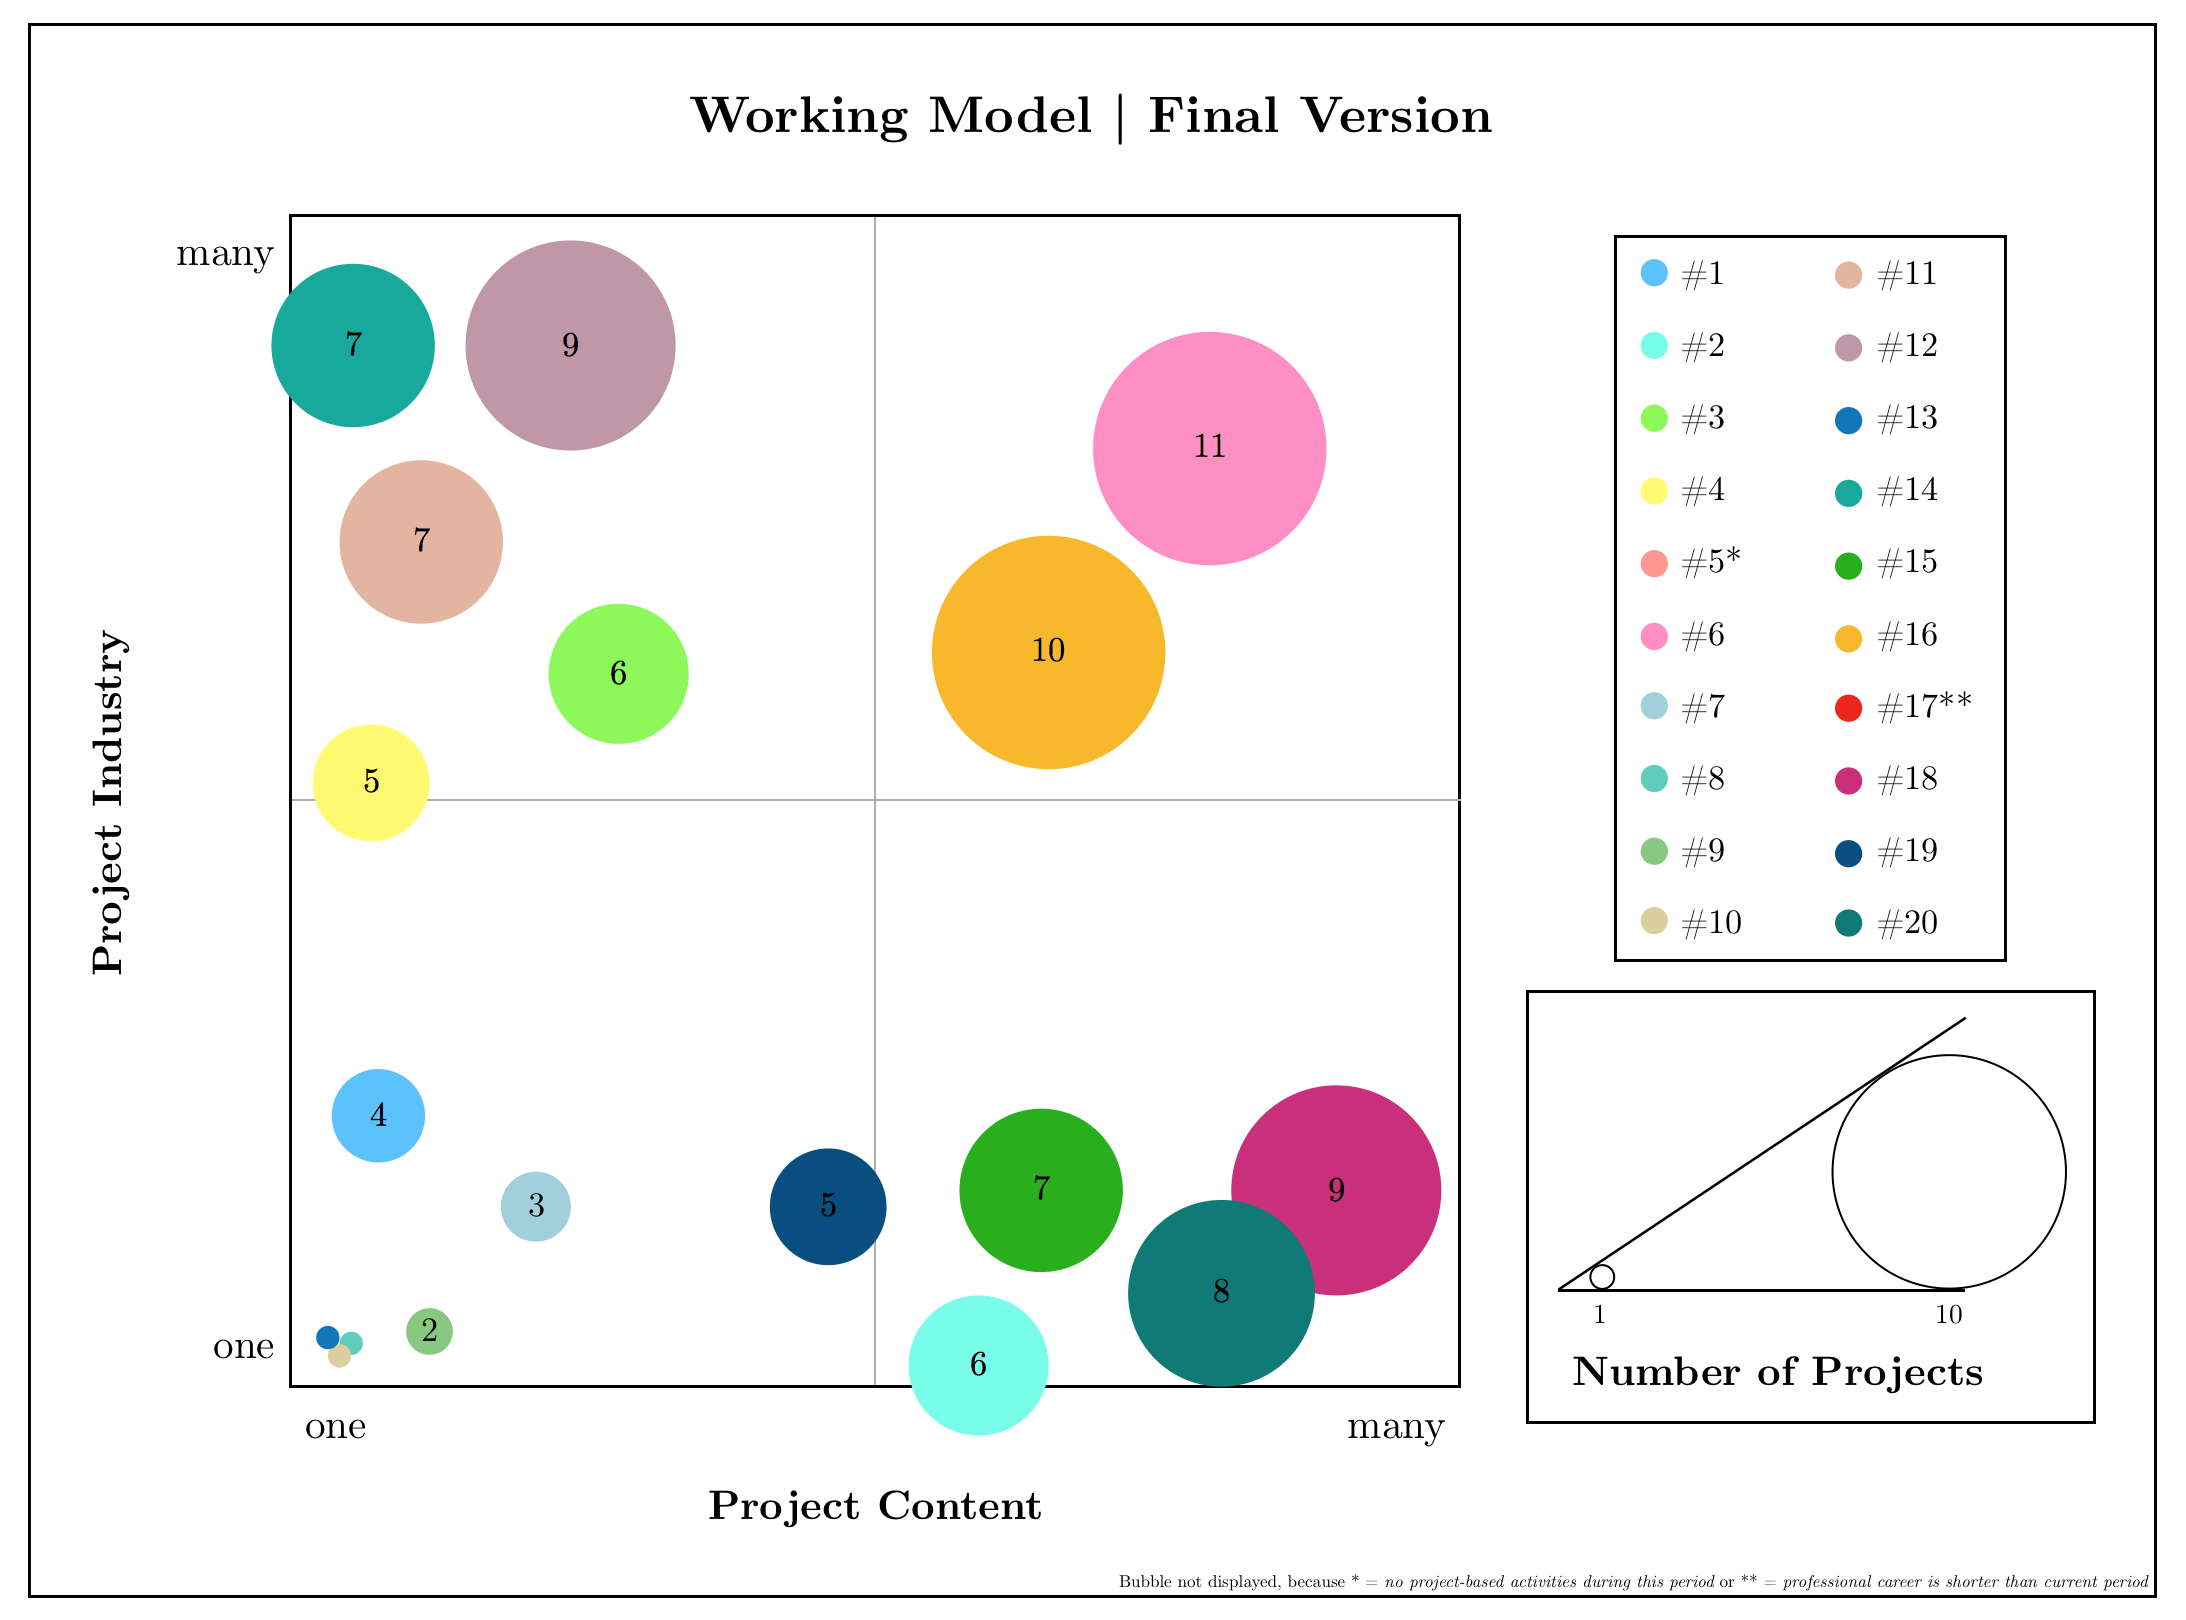
\includegraphics[width=.7\columnwidth]{figures/WM_final.png}
  \caption[The final working model]{The final working model – It comprises three dimensions, project industry ($y$-axis), project content ($x$-axis) and number of projects (bubble diameter and number), as well as a legend which allocates each colour to a candidate's ID (filled with dummy data).}
  \label{fig:final}
\end{figure}

The model exhibits three dimensions of the careers of project professionals. These dimensions are \textit{the number of different project industries}, \textit{the number of different project contents} and \textit{the total number of projects}. The analysis for these three attributes is conducted for periods of five years. This means, if the candidates interviewed have a work experience of 20 years or less, at the end of the analysis you'll have 4 models, one for the first five years, one for the period from the \nth{5} until the \nth{10} year, etc. For these periods the model depicts the attributes for all interviewees, which are differentiated by different colours. Furthermore, there were two reason why a candidate's bubble would not be displayed, the first one being that the candidate did no participate in project-related activities during this period (marked with one asterisk). The second one stands for the absence cause, that the interviewee's career is shorter than the corresponding period (marked with two asterisks). In the following, each of the three named dimensions of the working model are explained in detail.\\

\clearpage

\noindent {\bf Project industry}\\[.1cm]
The categorisation attribute \textit{project industry} is represented by the $y$-axis. Its scale was chosen to be non-numeric (one - many), since the non-numeric scale  allows for easier interpretation of the quadrants. However, the data is filled in based on a numeric scale. This scale was chosen considering the data sets. Therefore, the highest number of different industries within a time span of 5 years was ascertained, which led to a scaling of 1-5. The list of industries that was introduced in Chapter \ref{sec:LiteratureRev:PCategorisation:ByPIndustry} serves thereby as a theoretical structure by which in the analysis process the different industries of the projects in which the candidates worked in are identified and accordingly evaluated. \\

\noindent {\bf Project content}\\[.1cm]
The dimension \textit{project content} is located on the $x$-axis and alike the project industry-attribute its scale is non-numerical. Furthermore, the point's position is, similarly to the $y$-axis scaling, based on a linear scale, which was chosen according to the maximum value to be found in the data sets. As a result, the underlying numerical scale extends from 1 to 5. The differentiation between the various project contents of the project professionals follows the in chapter 2.2.1 introduced list of project contents by \citeA{patzak17}. At this point it is important to mention that the classification attribute 'project content' was not the initial sorting criteria as can be seen in figure \ref{fig:initial} on page \pageref{fig:initial}. Initially, the second dimension was 'project type'. However, the attribute was changed especially due to feedback received by the participants of the focus group workshop, which stated that project type as attribute is too broadly defined and that in the context of project professionals' careers 'project content' makes the most sense. This feedback is also backed by the project management literature, in which project types is used as hypernym for all the project attributes by which projects can be classified. \\

\noindent {\bf Number of projects}\\[.1cm]
In contrast to the other two dimensions the third dimension \textit{number of projects} is not represented by one of the axes, instead it is constituted by the diameter and the number written in the middle of each of the dots (except, if there is only one project). In order to be able to interpret the size of the dots a legend is shown on the right. For reasons of readability the maximum diameter size is limited to a 10 projects bubble and project numbers higher than 10 are only represented by the number in the middle. Furthermore, as can be seen in figure \ref{fig:initial} on page \pageref{fig:initial}, this dimension was not included in the initial model. 
It was added, as early analysis suggested that there may be other potentially relevant dimensions, of which number of projects was chosen as the most promising one. Above all, the third classification attribute was included in order to provide more depth to the model and thereby facilitate the interpretation of the outcomes. \\

\begin{figure}[!hbt]
    \captionsetup{font=small}
  \centering
  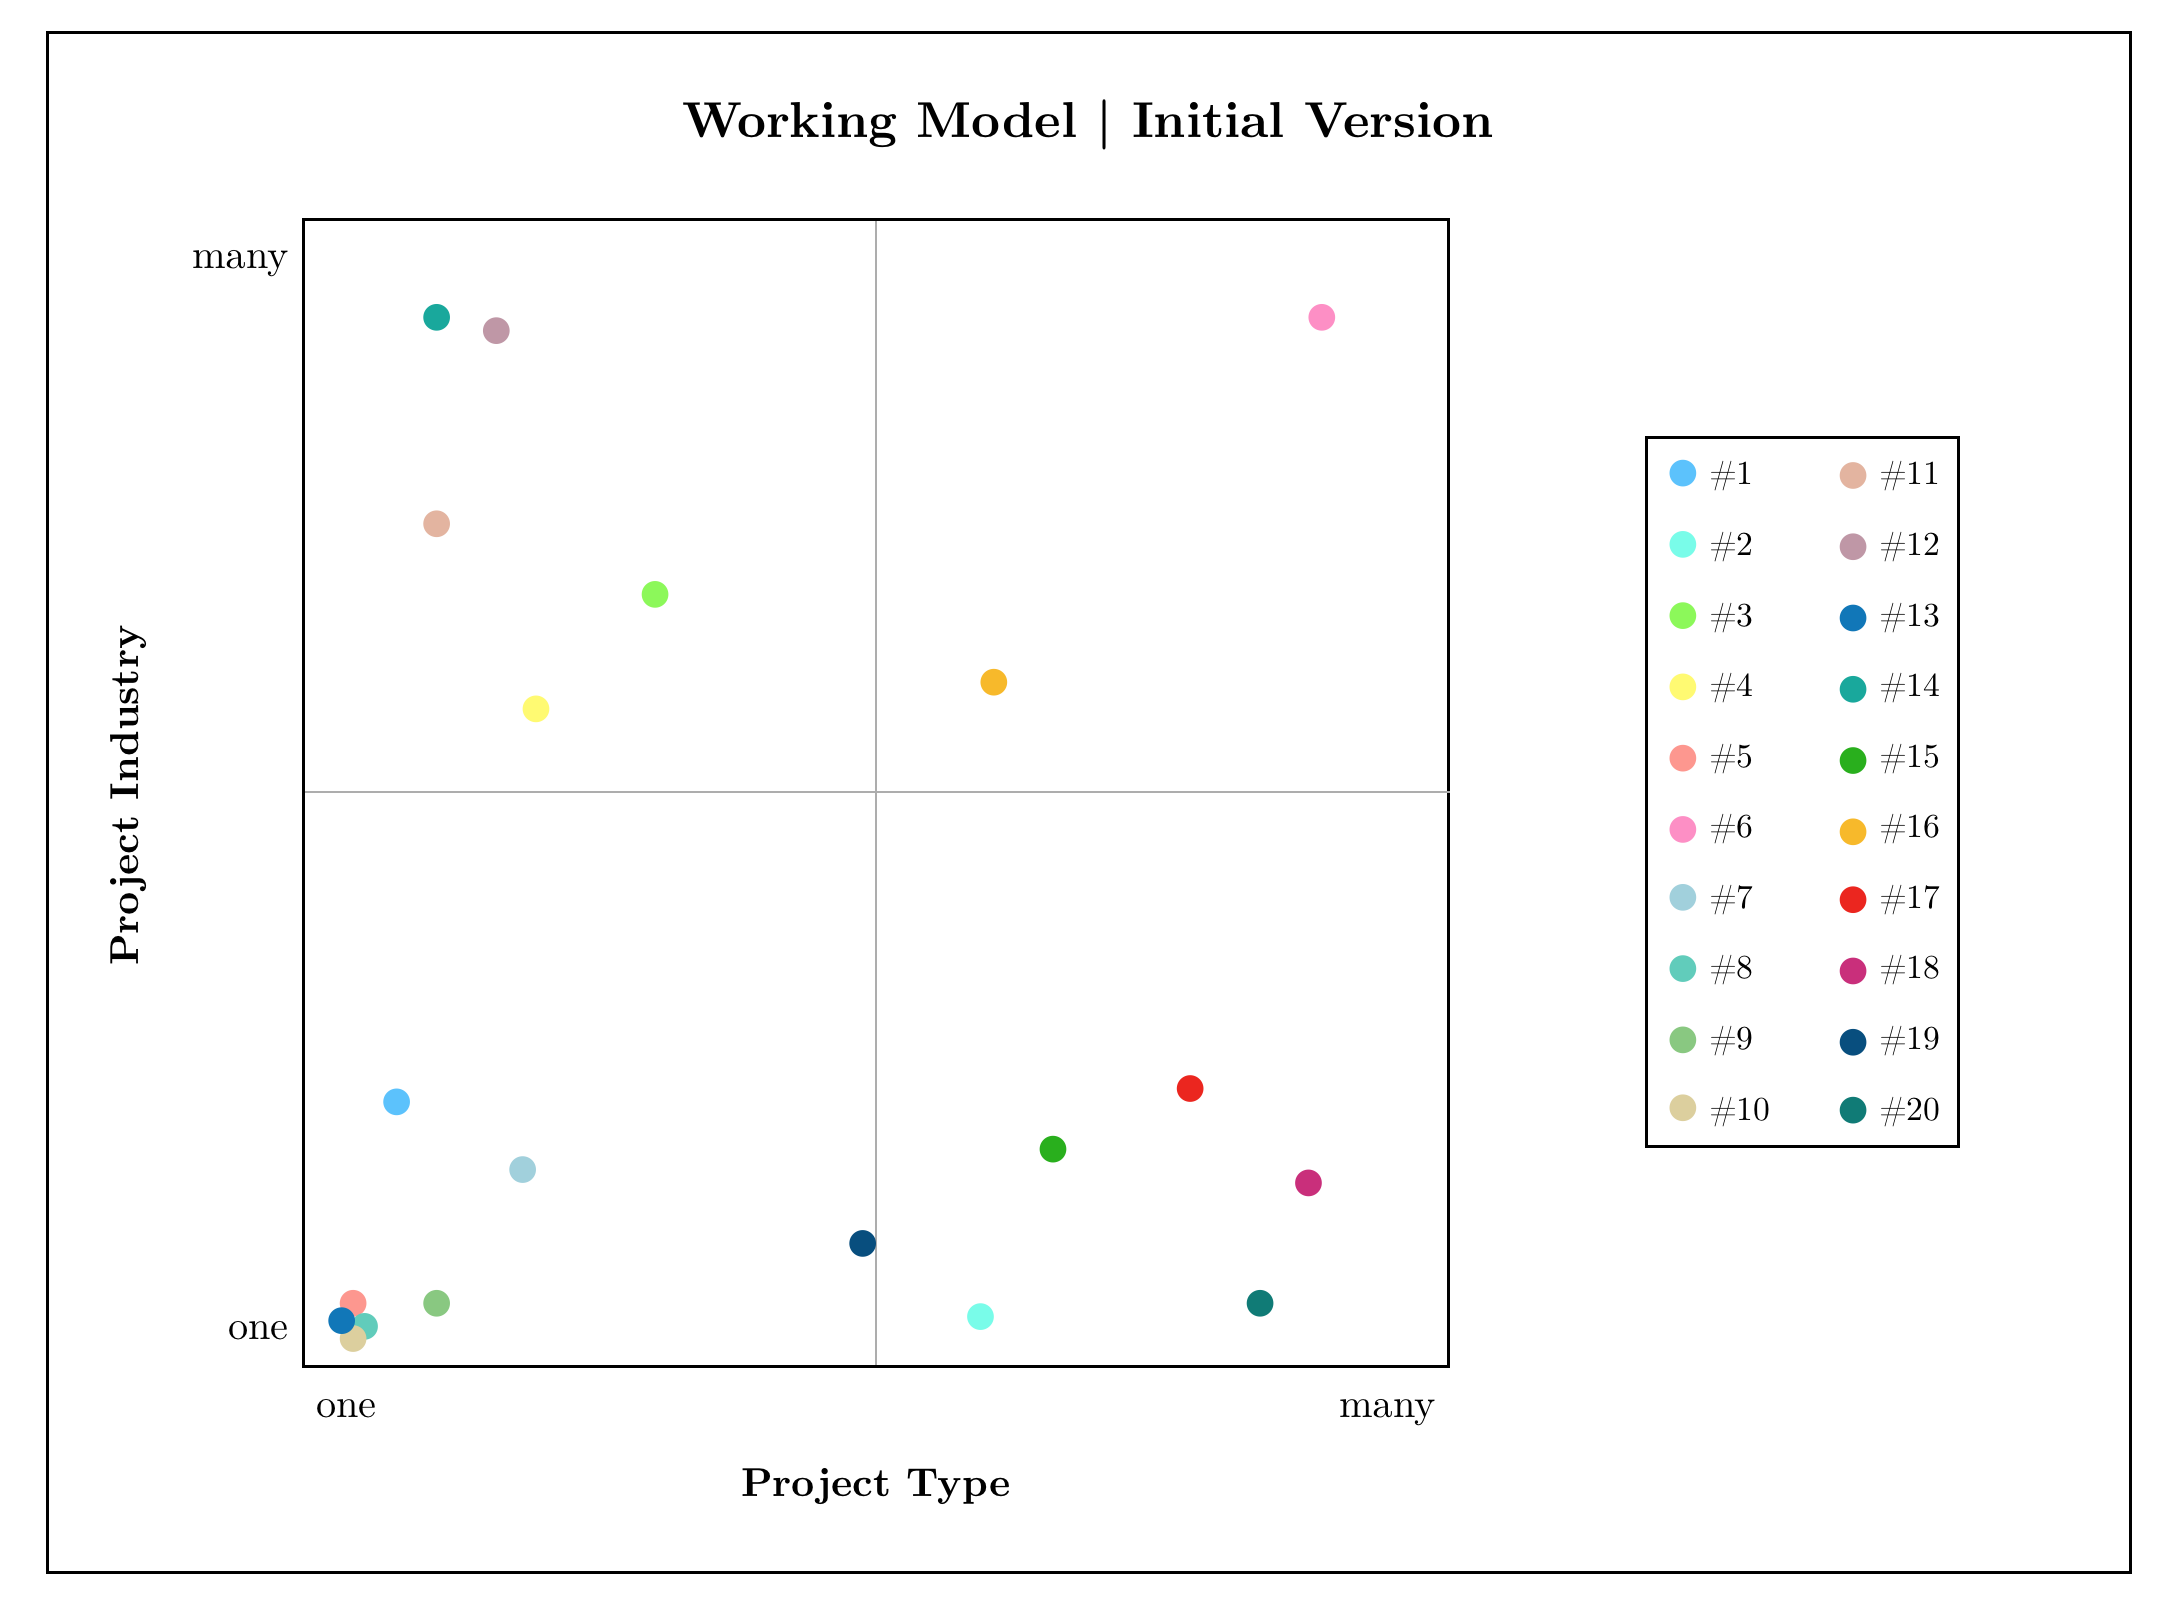
\includegraphics[width=.45\columnwidth]{figures/WM_Initial.png}
  \caption[The initial working model]{The initial working model (filled with dummy data).}
  \label{fig:initial}
\end{figure}

%\clearpage


\subsection{An alternate variant – The career movement model}
\label{sec:cmm}
The alternative variant of the final working model, \textit{The career movement model}, which is shown below in figure \ref{fig:alternate}, was included in this bachelor thesis, since it provides an interesting, different viewpoint on the research data. It includes, in contrast to the final model only the two main dimensions on the axes. Instead of the third dimension, it shows for each candidate, his/her position in the map during each of the five-year periods since the start of his/her professional career. In other words, it makes movements of a project professional during his/her career in respect to project content and industry visible and is therefore named career movement model. In detail, each of the dots represents one of the periods and the number indicates which it was (1: 0-\nth{5} year, 2: \nth{5}-\nth{10} year, etc.). As a result, it enables the researcher, on the one hand, to compile the stages of the project professionals' career to see them all in one model, in contrast to the final model. Furthermore, it uncovers periods in a project professional's career in which he/she did not work in projects at all. This is visualised by a missing dot and the corresponding number, as can be seen for explanatory purposes in figure \ref{fig:alternate} where in candidate 3's career path the \nth{3} stage is missing. In order to make it visible if a project professional did not do any projects at all in the last periods of his/her career, in this case one grey bubble(s) with the corresponding number for each period is added to the last project bubble. Above all, it facilitates the comparison during the analysis process of the careers of project professionals among themselves and in between different industries, as well as regarding other candidate specific criteria. Thereby, this variant contributes to one of the core research questions of finding patterns in project professional's careers. \\


\begin{figure}[!hbt]
    \captionsetup{font=small}
  \centering
  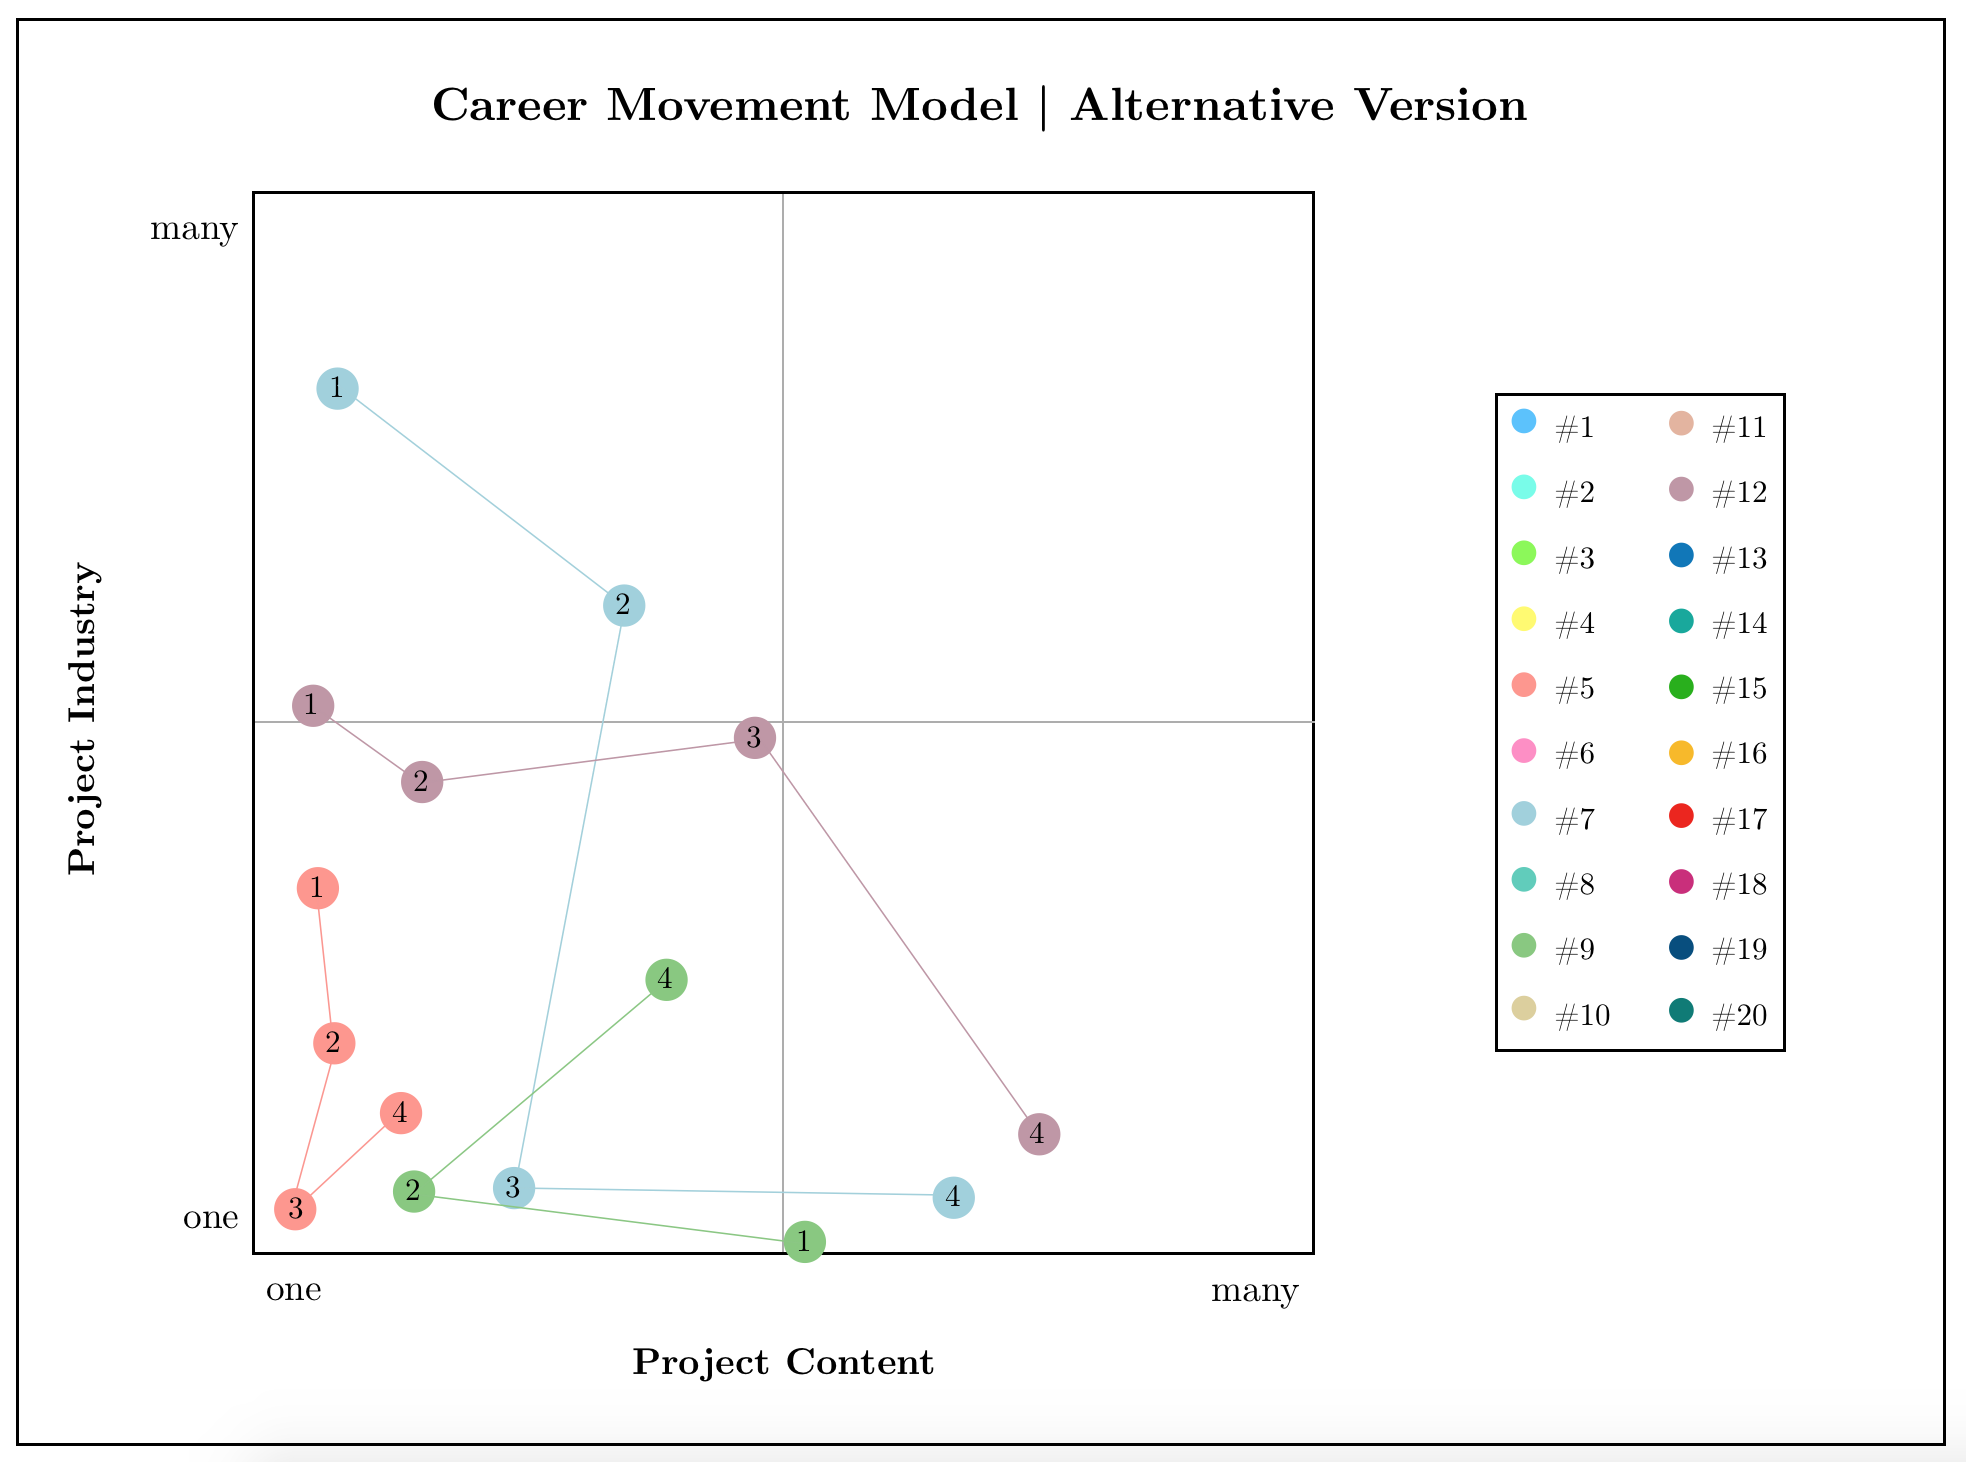
\includegraphics[width=.7\columnwidth]{figures/WM_alternate.png}
  \caption[The career movement model]{The career movement model – An alternative variant of the final working model. It comprises the same axes dimensions, project industry ($y$-axis) and project content ($x$-axes), but instead of the third dimension, it shows the position for each of the career periods, indicated by the number in the bubble (filled with dummy data).}
  \label{fig:alternate}
\end{figure}


\cleardoublepage

\section{Study}
\label{sec:study}
After the presentation of the final working model, in this chapter the results of the analysis of the study data using it is depicted. Before that the sample group is presented in detail and the outcomes of various the main analysis accompanying evaluations are presented. These accompanying analyses serve the purpose of underpinning the results of the main working model with relevant results, and therefore, enriching and facilitating the discussion of the outcomes, which is held in the following chapter.

%————————————————————–––––––––––––––––––––––––––———————————————————
%————————————————————–––––––Subsection–1————––––––––———————————————

\subsection{Sample group}
In order to get a better understanding of the obtained results, it is important before looking at the actual study outcomes to look at some key figures regarding the sample group, which will be provided in the following. As can be seen in table \ref{tab:candid}, which provides key indicators for each candidate, on page \pageref{tab:candid} the sample group is mostly made up by male project professional. This fact could be partly attributed to the high share of interviewees with an IT background, which is a sector known to have unequal distribution of genders \cite{harrington15}. Another crucial factor for this thesis is the age of the candidates and the corresponding years of professional experience. As table \ref{tab:candid} shows, is the mean value, as well as the median for both indicators relatively high (Age $\bar{x}$: 47 | $\tilde{x}$: 49; Professional experience $\bar{x}$: 21,8 | $\tilde{x}$: 22,5). This can be explained by the determining factor that at the beginning of this exploratory study mostly project professional in senior level were interviewed.\\

\begin{table}[!hbt]
\centering
\captionsetup{font=small}
\footnotesize
    \begin{tabular}{|c|c|c|c|c|}
    \hline
    ID   & Gender                 & Current industry & Age (yrs.)        & Prof. Experience (yrs.) \\ \hline
    \#1  & Female                 & Consulting                     & 38                & 19                      \\ \hdashline
    \#2  & Male                   & Manufacturing                  & 55                & 35                      \\ \hdashline
    \#3  & Male                   & IT                             & 58                & 29                      \\ \hdashline
    \#4  & Male                   & IT                             & 62                & 40                      \\ \hdashline
    \#5  & Male                   & Financial services/insurance   & 36                & 10                      \\\hdashline
    \#6  & Male                   & IT                             & 49                & 23                      \\\hdashline
    \#7  & Male                   & IT                             & 37                & 14                      \\\hdashline
    \#8  & Male                   & IT                             & 57                & 25                      \\\hdashline
    \#9  & Male                   & IT                             & 45                & 20                      \\\hdashline
    \#10 & Male                   & IT                             & 36                & 12                      \\\hdashline
    \#11 & Male                   & IT                             & 48                & 23                      \\\hdashline
    \#12 & Male                   & IT                             & 60                & 40                      \\\hdashline
    \#13 & Female                 & IT                             & 31                & 8                       \\\hdashline
    \#14 & Male                   & IT                             & 55                & 32                      \\\hdashline
    \#15 & Male                   & Electronics                    & 49                & 22                      \\\hdashline
    \#16 & Male                   & Infrastructure                 & 43                & 17                      \\\hdashline
    \#17 & Female                 & Infrastructure                 & 52                & 24                      \\\hdashline
    \#18 & Male                   & IT                             & 25                & 7                       \\\hdashline
    \#19 & Male                   & IT                             & 49                & 24                      \\\hdashline
    \#20 & Male                   & Infrastructure                 & 60                & 29                      \\ \hline
         & 85 \% M | 15\% F & 65\% IT | 15\% Infrastructure  & $\bar{x}$: 47 | $\tilde{x}$: 49 & $\bar{x}$: 21,8 | $\tilde{x}$: 22,5 \\  \hline
    \end{tabular}
    \caption[Key data about candidates]{Key data about candidates.}
    \label{tab:candid}
\end{table}

\clearpage






%————————————————————–––––––––––––––––––––––––––———————————————————
%————————————————————–––––––Subsection–2————––––––––———————————————

\subsection{Results}
As indicated in the introduction to this chapter, this section presents the results of various analyses. It is divided into two parts. In the first part the results of the main working model, as well as, concomitantly conducted analyses are described. The second subsection showcases the results of the application of the in chapter 3 introduced career movement model.

\subsubsection{From the working model}


%——————————————–––––—————The–main–working–model–––––———————————————————

As described before in the \nth{3} chapter, the final working model can be used to evaluate the careers of project professionals regarding the three dimensions project industry, project content and number of projects. The first step of this evaluation process was to analyse each interviewee's data set for these three factors and in then to insert the data into the working model. The corresponding result of this process can be seen in figures \ref{fig:WM_0005}–\ref{fig:WM_2025} on page \pageref{fig:WM_0005}. Each figure hereby constitutes the sample group positioning for one career period.

On first sight, it an be seen in figure \ref{fig:WM_0005}, constituting the first five years of a project professional's career, that out of the 19 displayed project professionals the majority (14) focuses on either doing only one project type or projects in one project industry, instead of doing multiple project contents in multiple project industries at the same time. Furthermore, it can be seen that of the ones, differentiating by only one of the two dimensions, more (six vs. three) do one project content in multiple industries.
In the second period, displayed in figure \ref{fig:WM_0510}, this aspect changes completely as the majority (four vs. one) of the candidates, differentiating only by one dimension, diversify by doing multiple project contents instead of industries. Moreover, a reduction of the number of projects conducted can be observed as in the first 5 years 42\% of interviewees did 10 or more projects, in comparison to 27\% in the years from 5 to 10. This goes a long with a concentration of the ones doing multiple project contents and industries along the diagonal line from the bottom-left to the top-right. This means that they did in this period multiple project contents in multiple project industries, rather than doing only one or few of one category and multiple of the other one, like in the first term.
This described trend levels off again in the third period, as can be seen in figure \ref{fig:WM_1015}. Furthermore, 77\% of the displayed candidates is located directly along one of the two axes, which implies that they did in only one category more than one distinct project type. 
In the fourth career period, constituted by figure \ref{fig:WM_1520}, almost half (46\%) of the candidates do three project contents and/or projects in three project industries, but in return none does more than this. Apart from this aspect, the relative share of them, who do 10 or more projects decreases further to 23\% in relation to period 2.
The fifth and last term, pictured in figure \ref{fig:WM_2025}, shows a relatively balanced constellation, despite the fact, that none of the project professionals can be found above the before named diagonal line, what means that none of them does more project industries than he does project contents. In general it can be observed that the number of candidates gets less over time, being only seven in the last period, which originates, as described in the previous subsection, from the fact that the majority of the sample group has less than 25 years of experience, and with some even having less than 10 years. 

As could be derived from the short descriptions of some outstanding aspects, this model visualises a lot of different constellations and movements all in one, therefore a series of analyses from singular perspectives were conducted in the following in order to make the results more comprehensive to the reader. The completed analyses can be categorised by three factors, which are \textit{Period oriented}, \textit{Project oriented} and \textit{Individual oriented}. These determining factors are used in the following as a guiding thread for the presentation of the conducted analyses and their outcomes. \\




\begin{figure}[!hbt]
    \captionsetup{font=small}
  \centering
  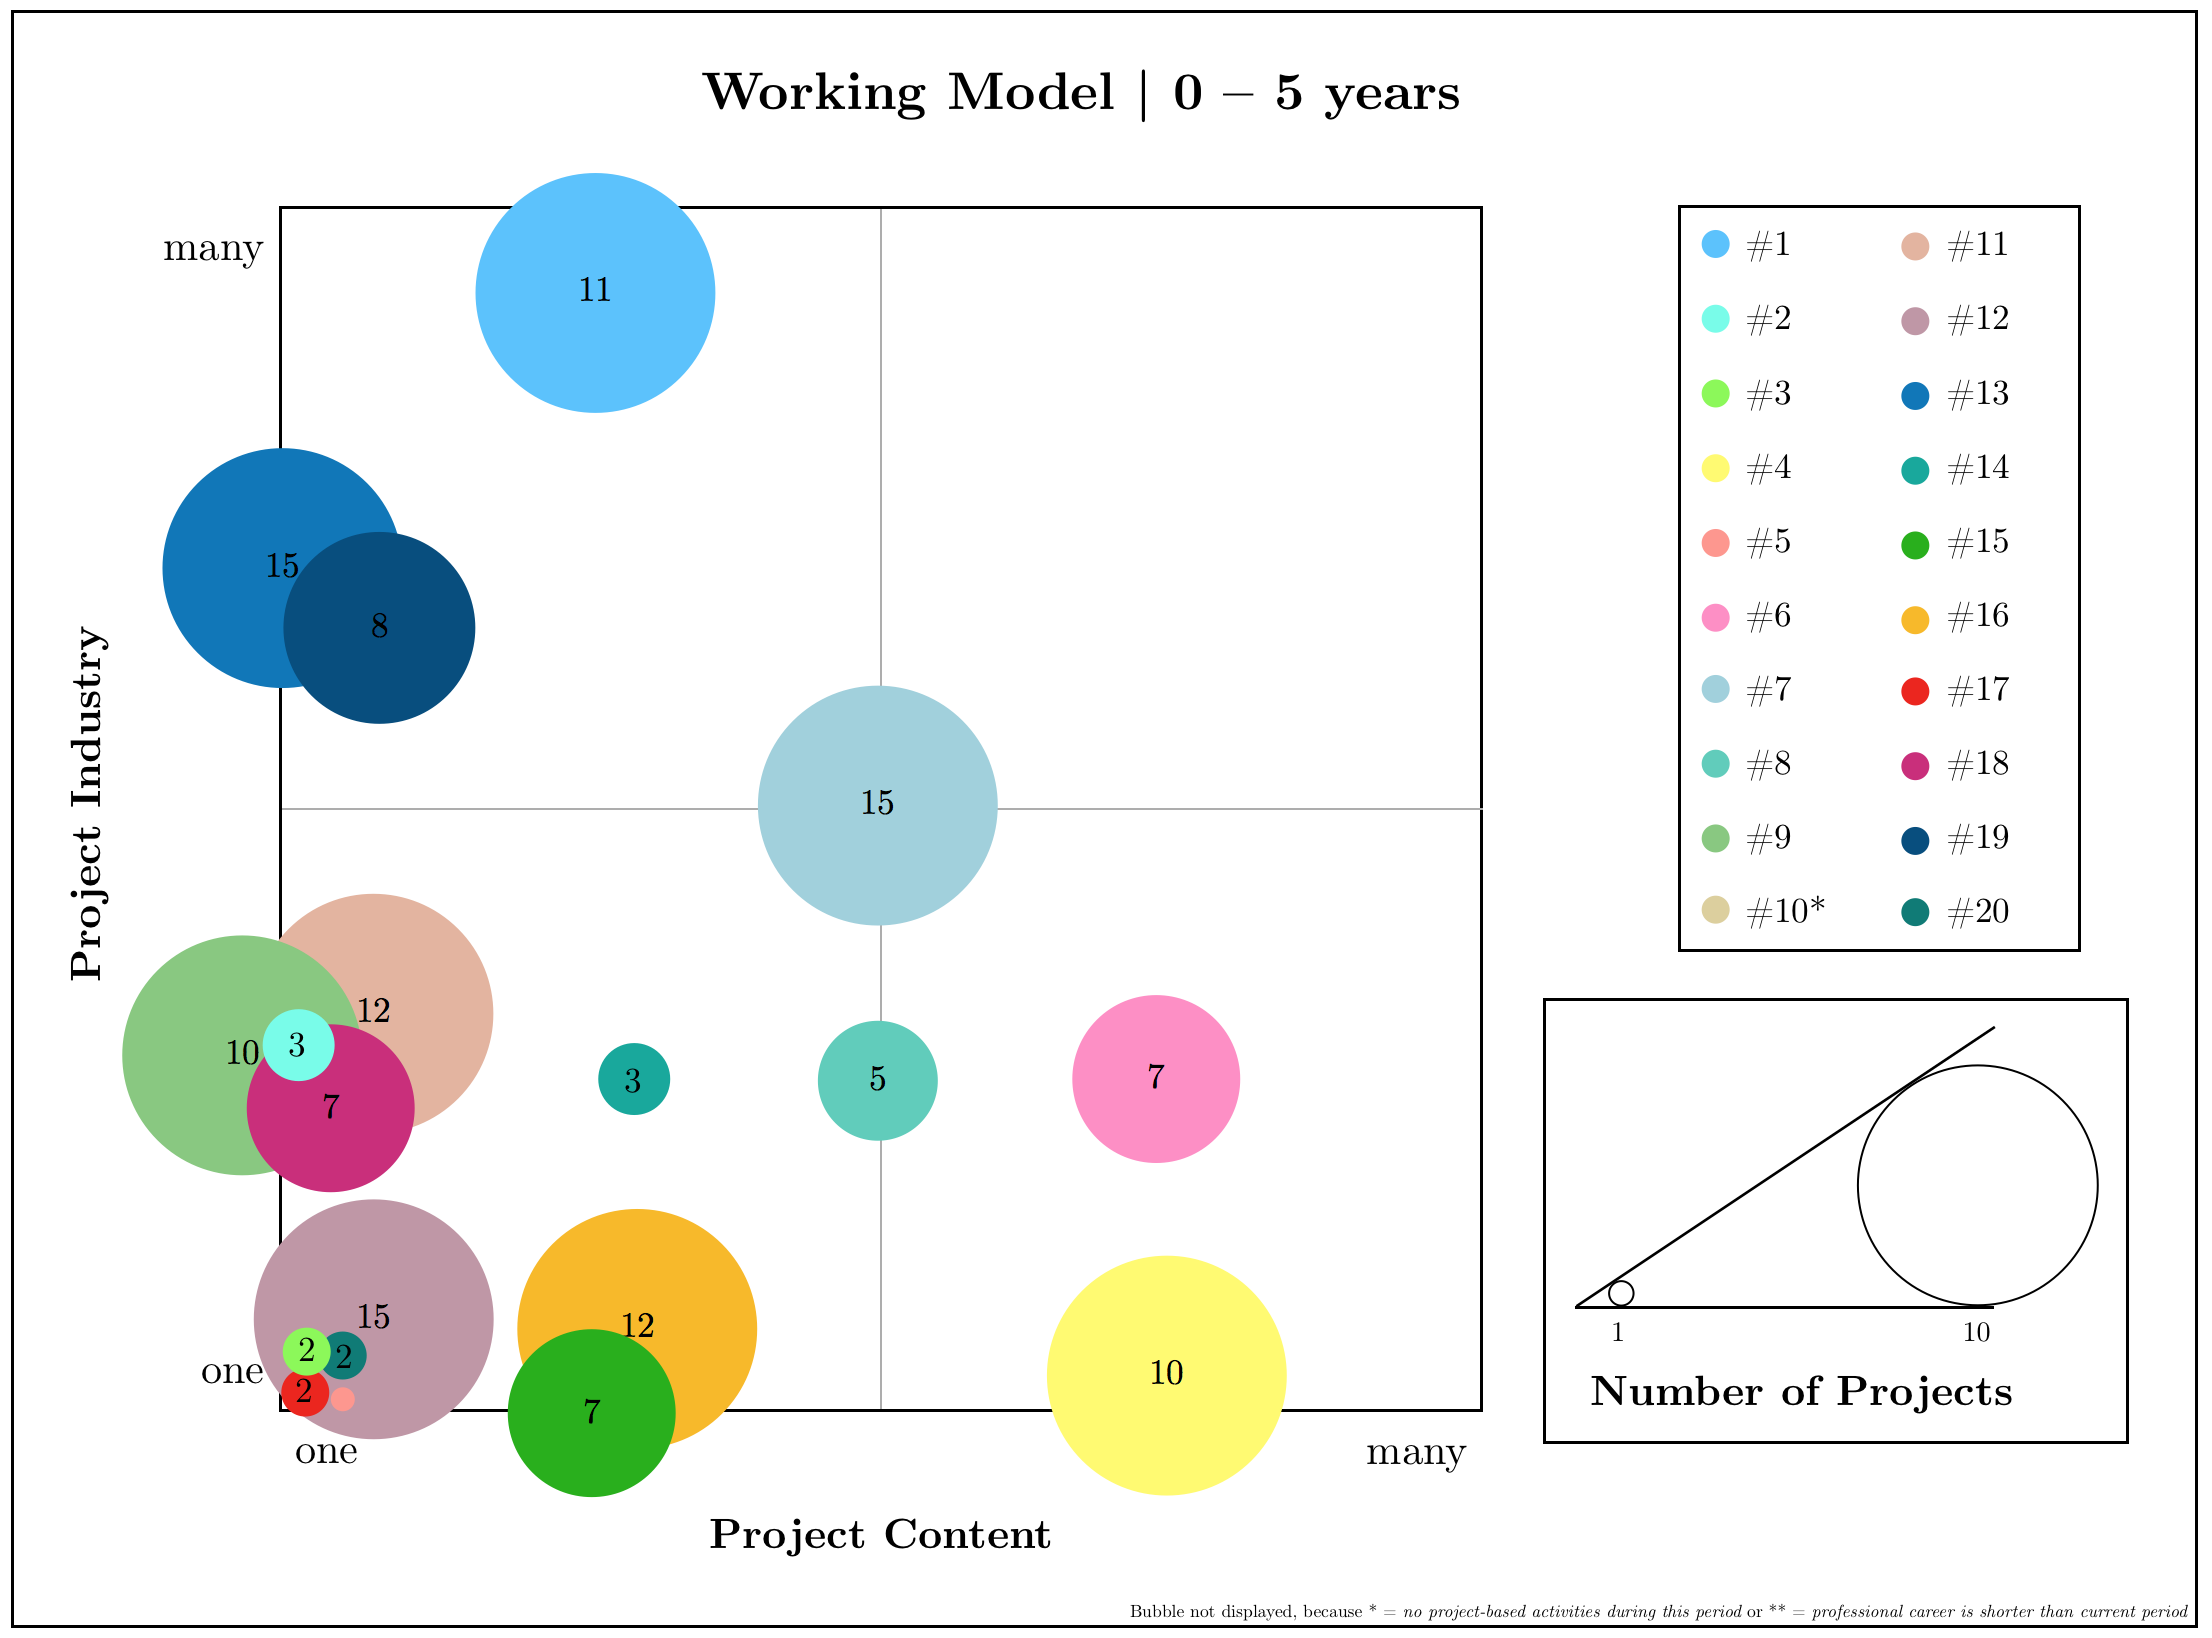
\includegraphics[width=0.75\columnwidth]{figures/WM_0005.png}
  \caption[Results of the working model: 0–5 years]{Results of the working model for the \nth{1} career period (0 – 5 years)}
  \label{fig:WM_0005}
  
\vspace*{.6cm}

\minipage[t]{0.48\textwidth}
  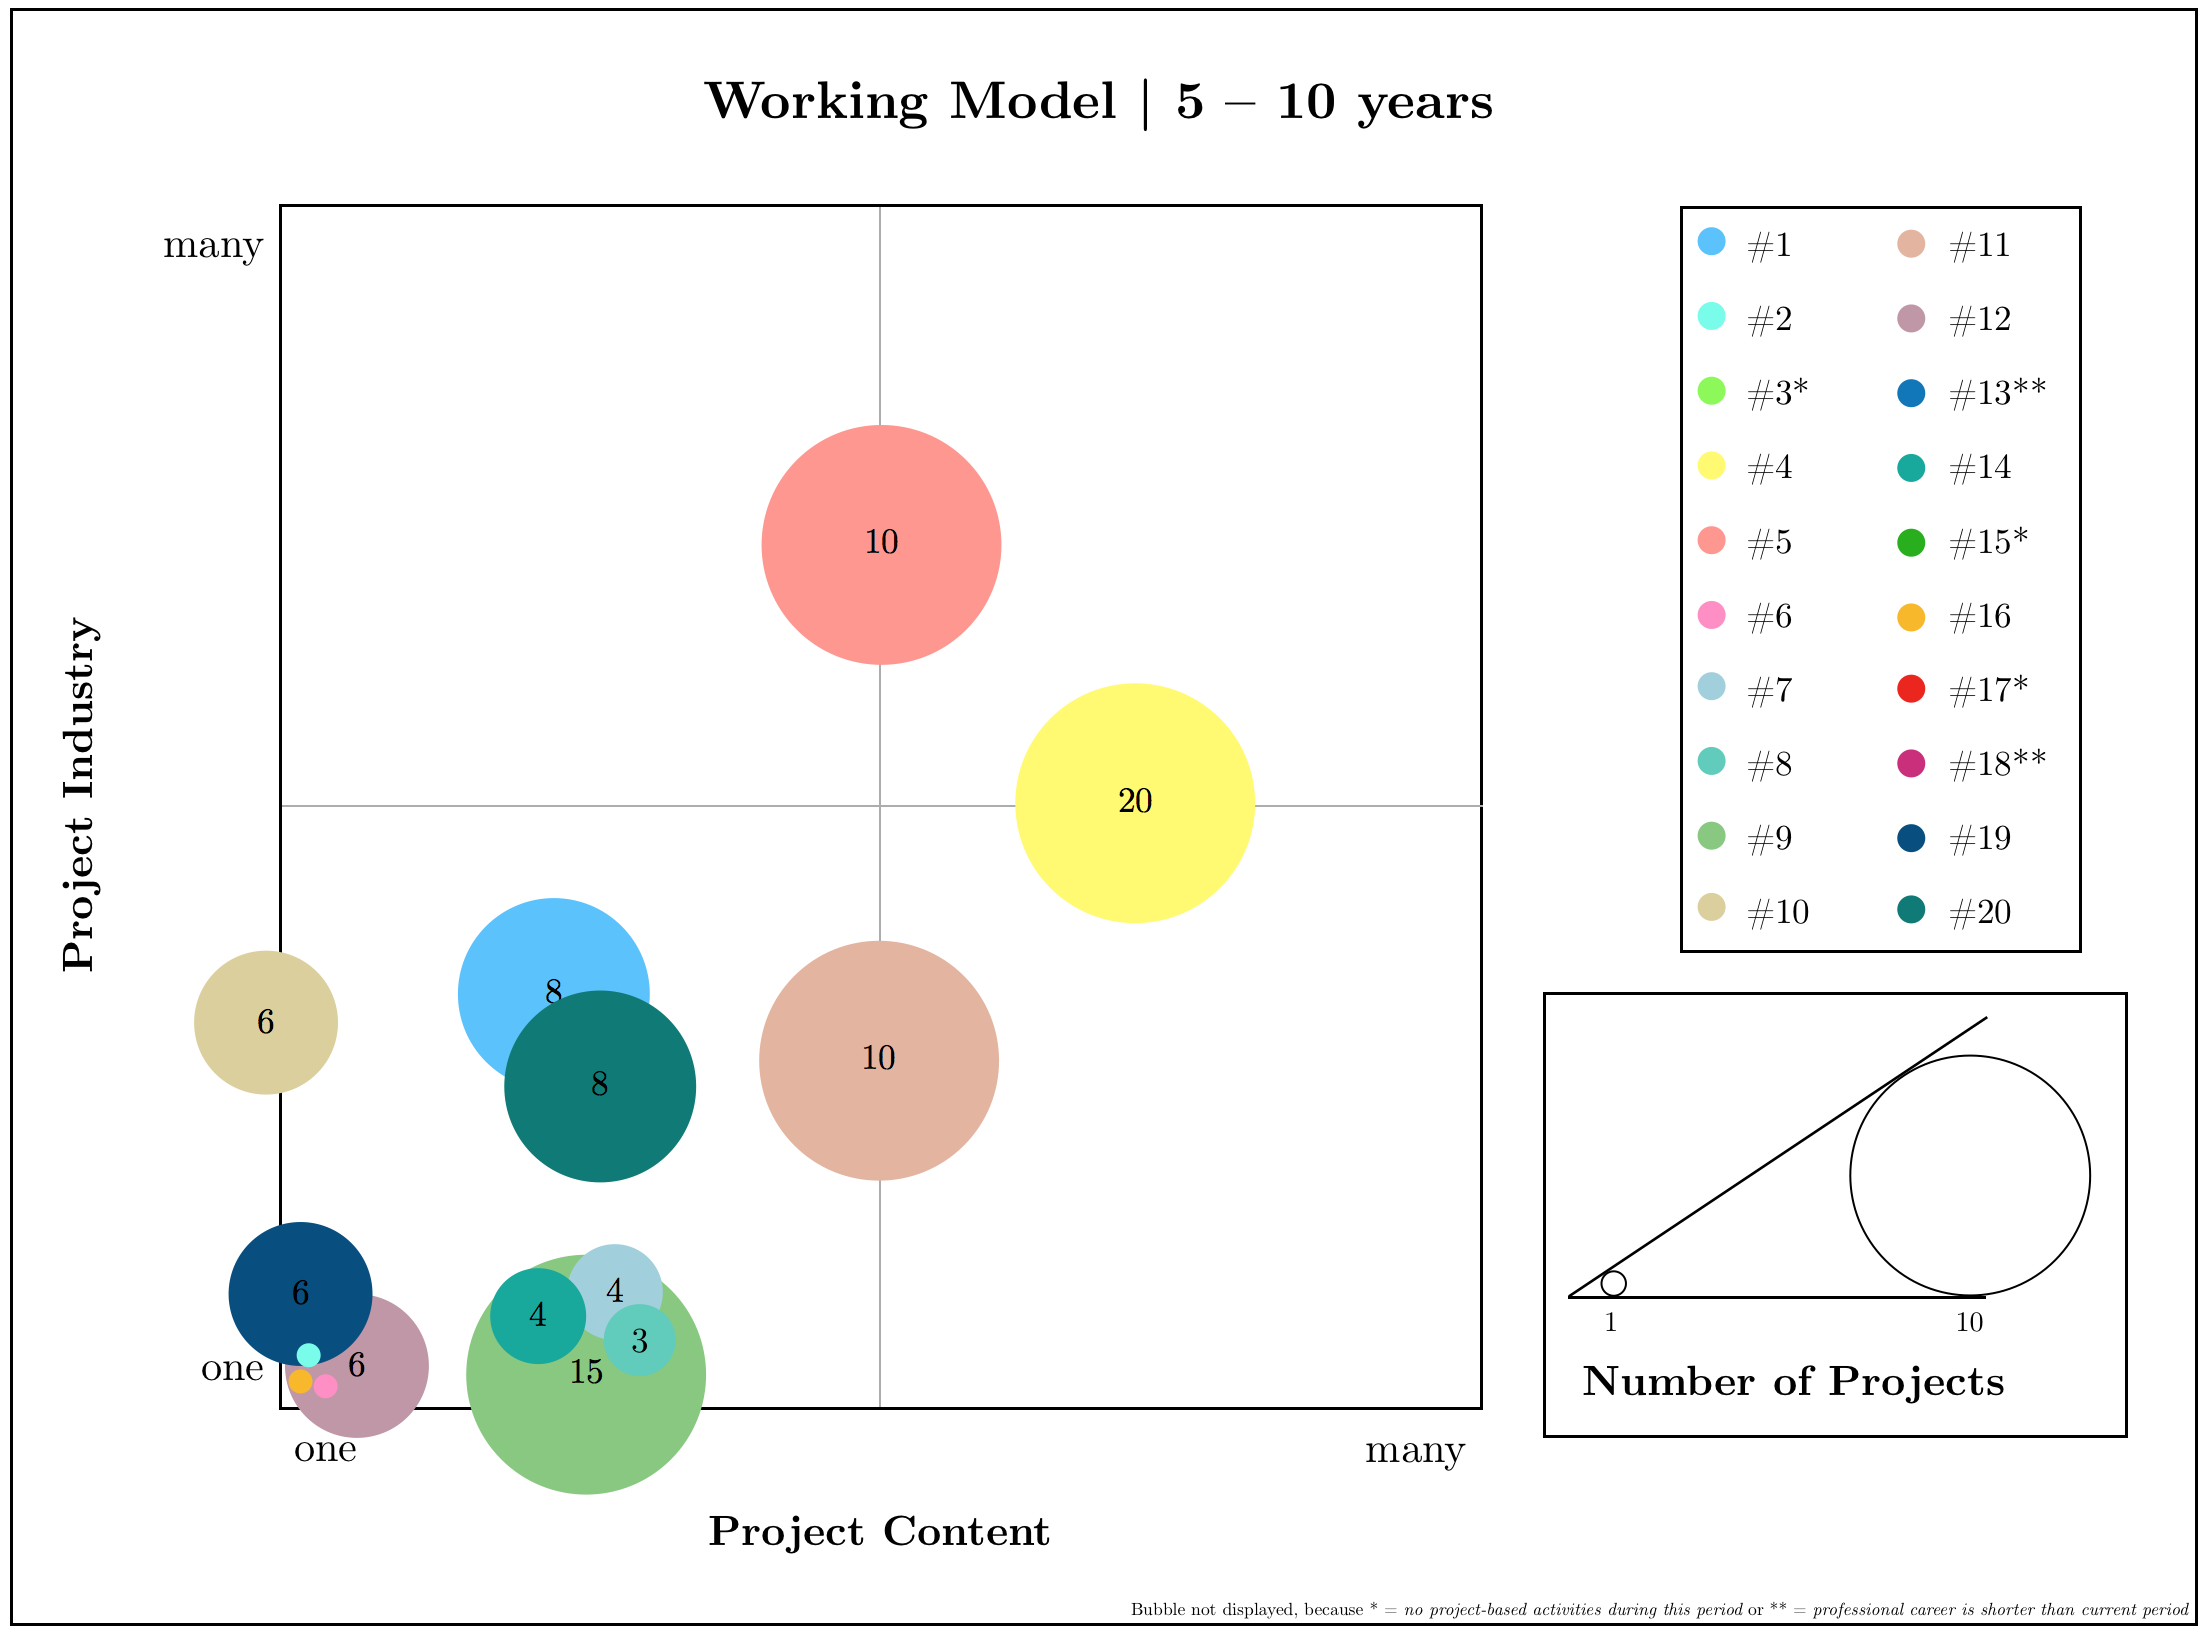
\includegraphics[width=\linewidth]{figures/WM_0510.png}
  \caption[Results of the working model: 5–10 years]{Results of the working model for the \nth{2} career period (5–10 years)}
  \label{fig:WM_0510}
\endminipage\hfill
\minipage[t]{0.48\textwidth}
  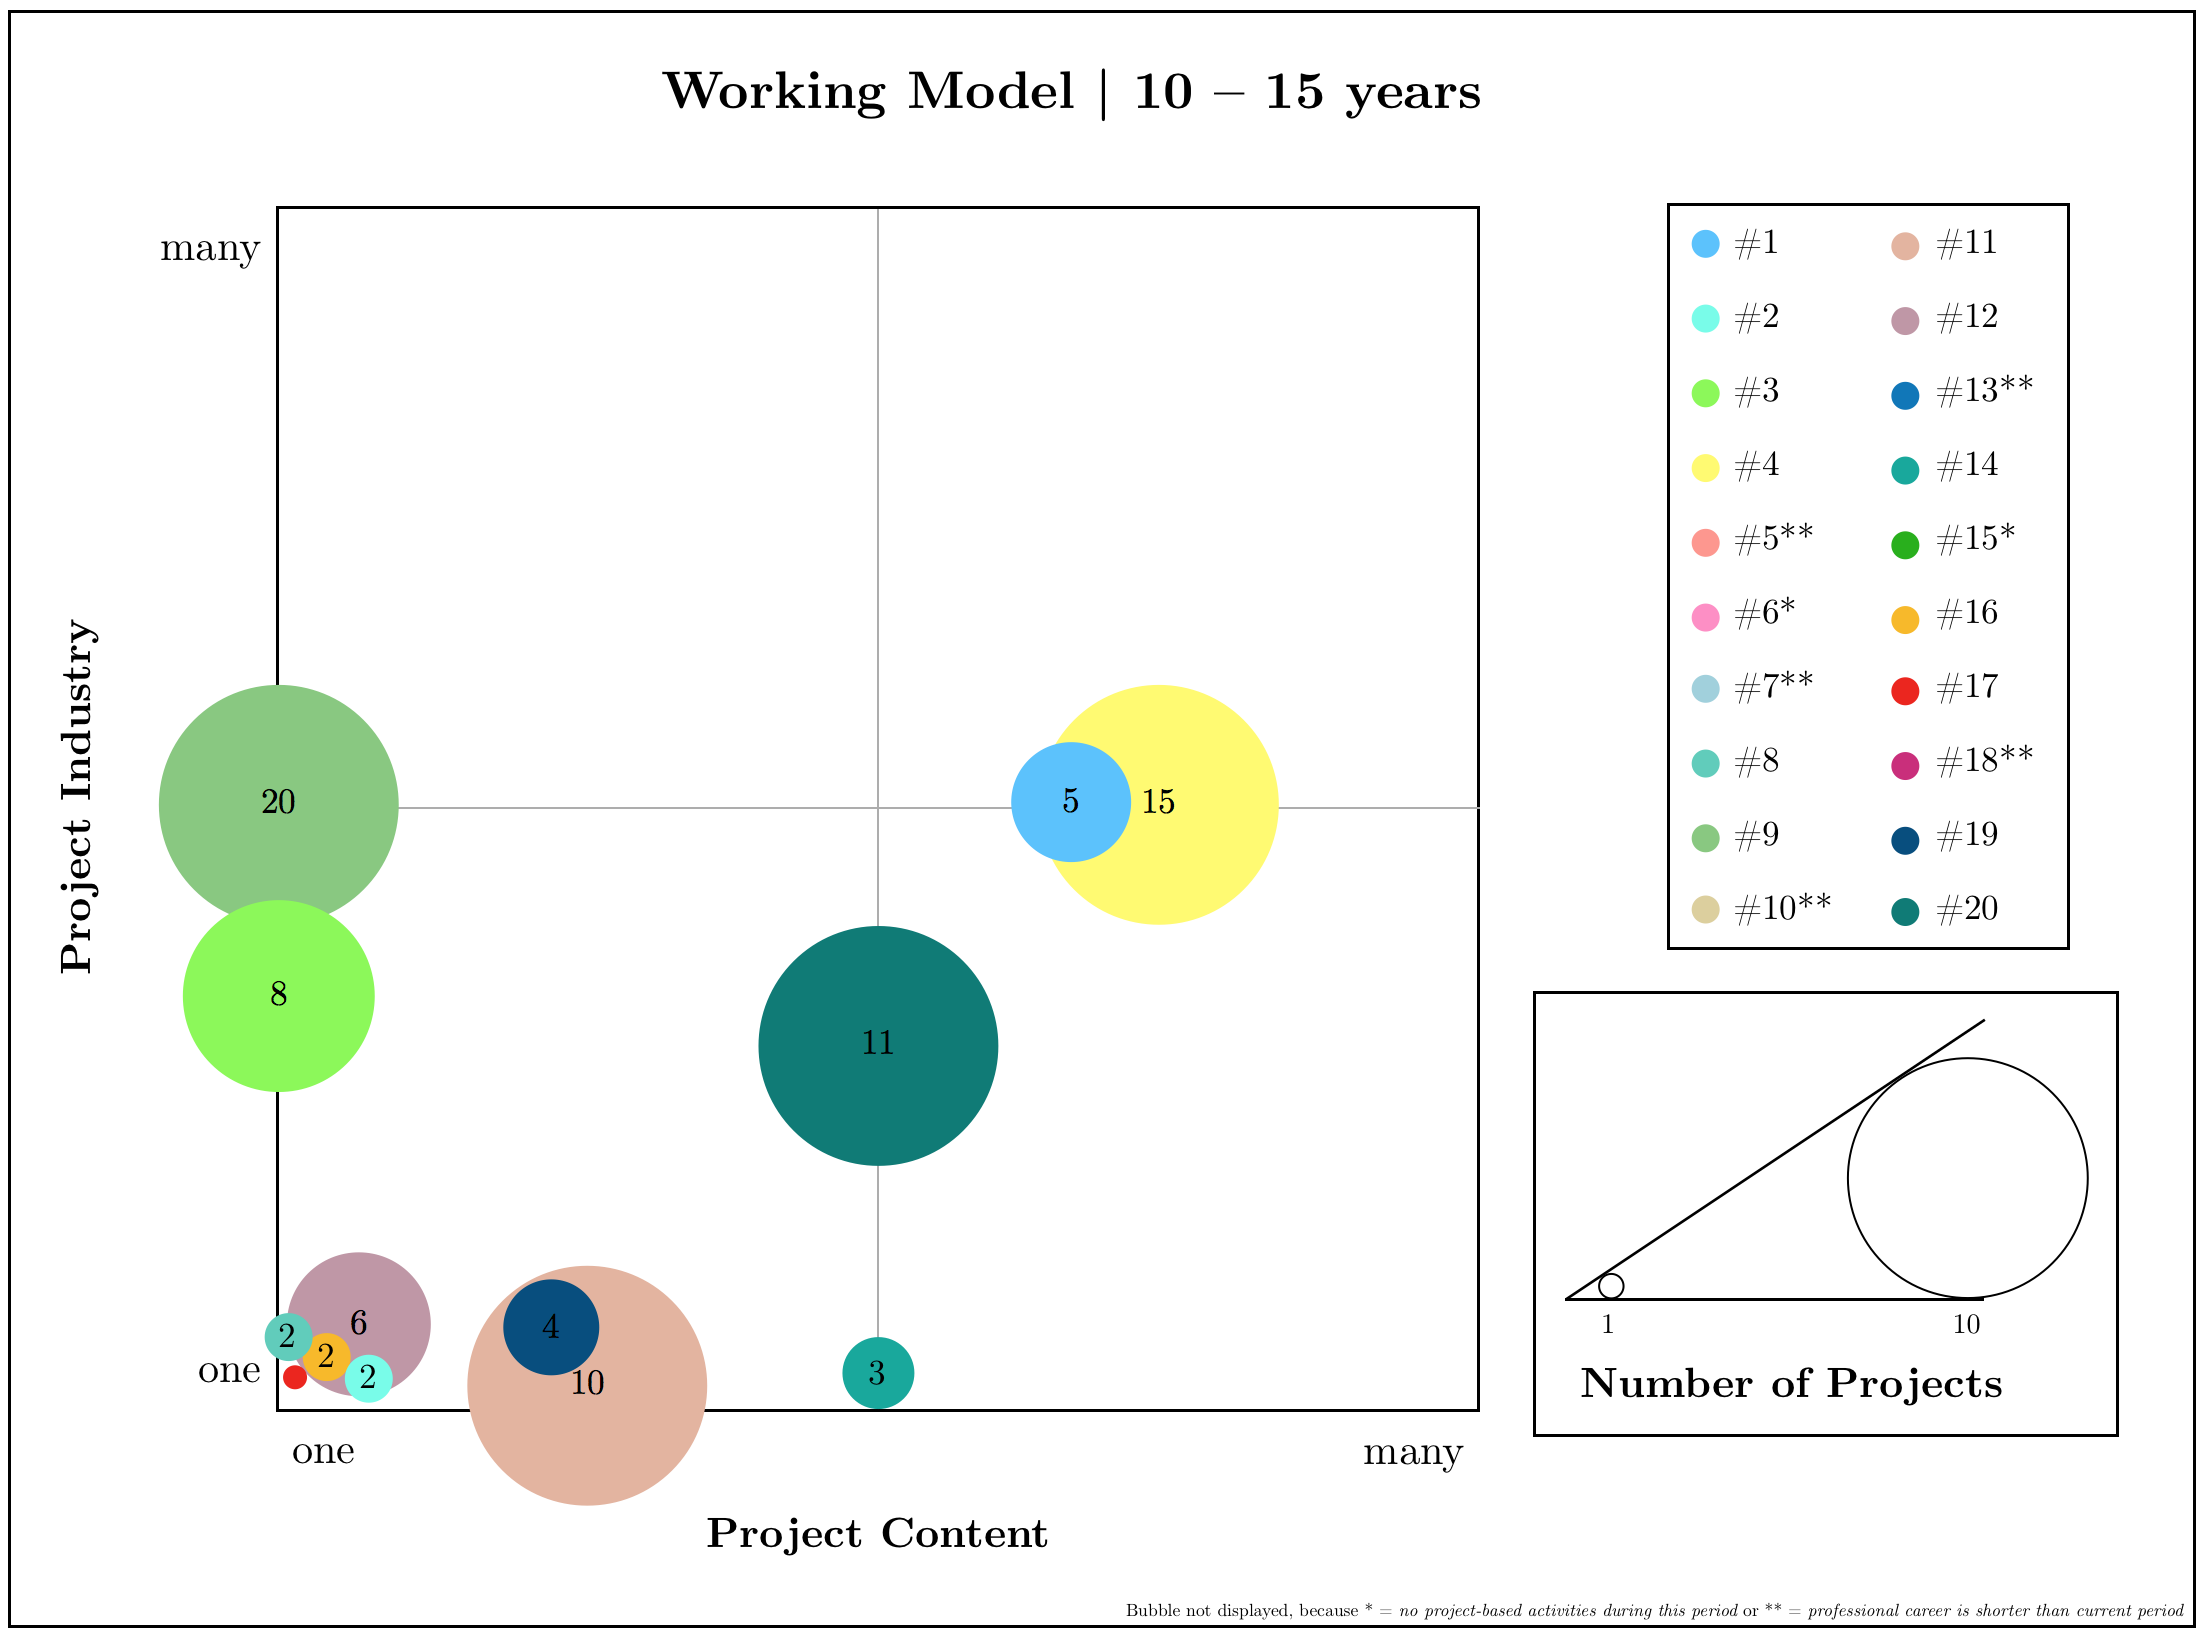
\includegraphics[width=\linewidth]{figures/WM_1015.png}
  \caption[Results of the working model: 10–15 years]{Results of the working model for the \nth{3} career period (10–15 years)}
  \label{fig:WM_1015}
  \endminipage

\vspace*{.6cm}

\minipage[t]{0.48\textwidth}
  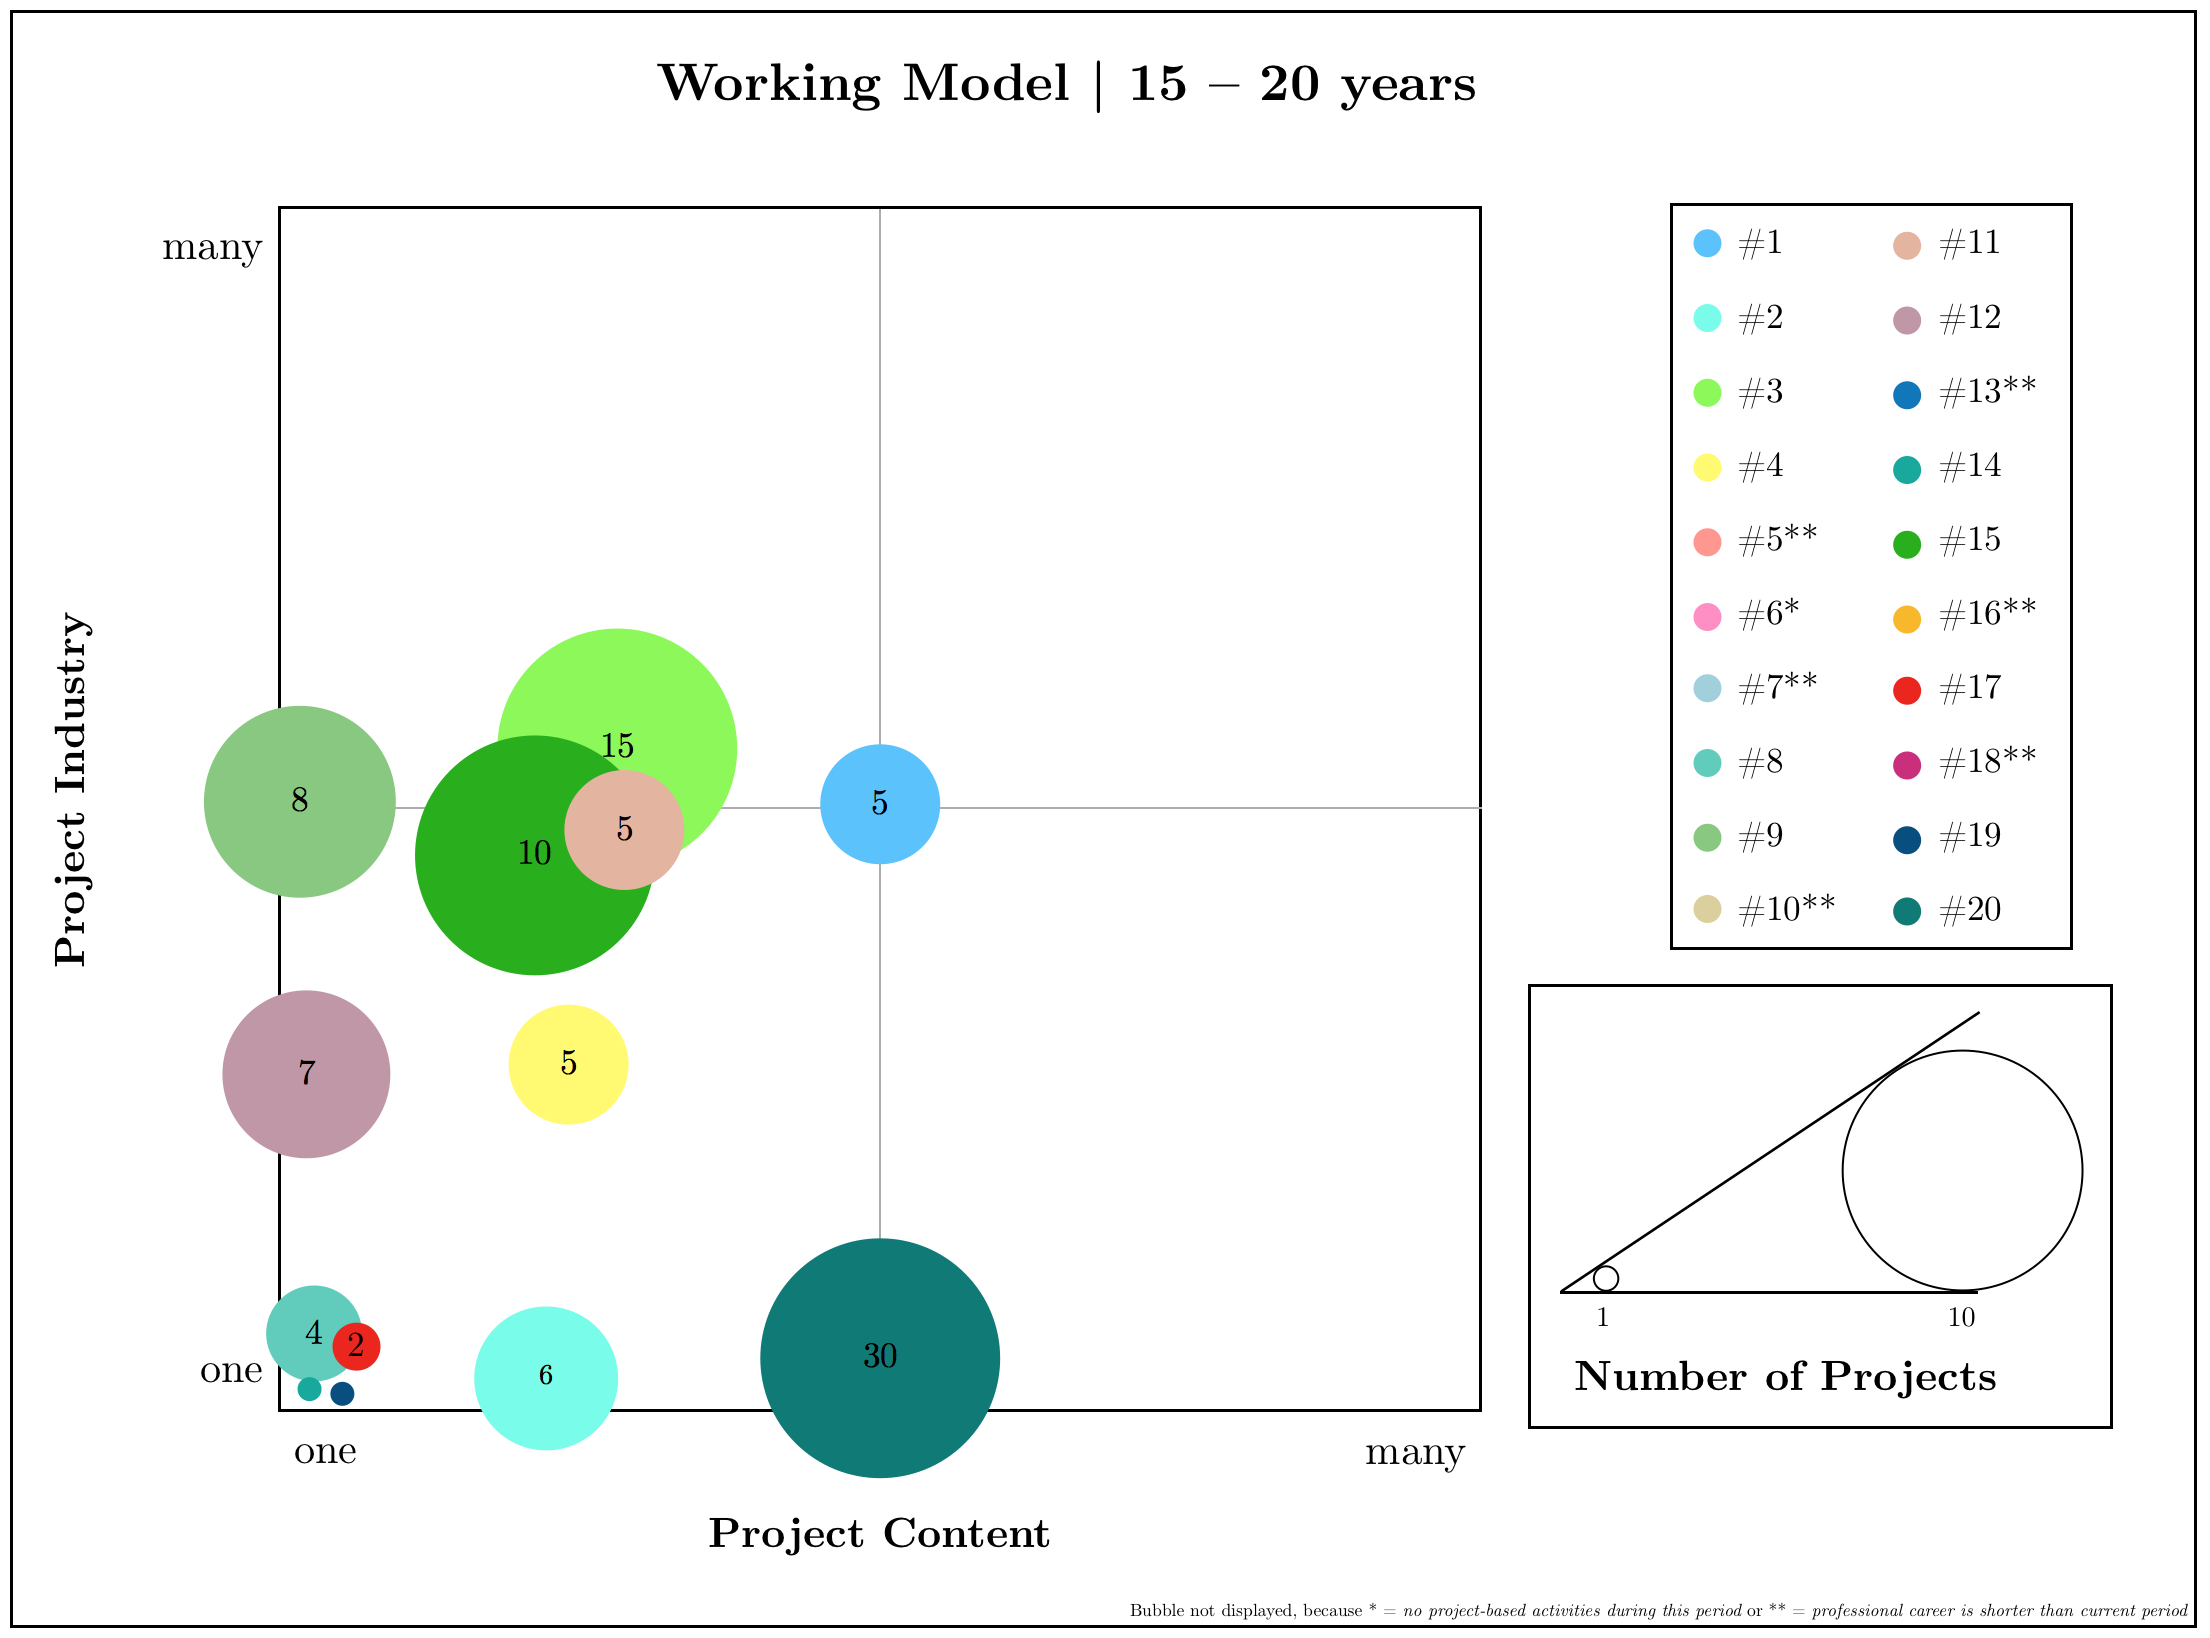
\includegraphics[width=\linewidth]{figures/WM_1520.png}
  \caption[Results of the working model: 15–20 years]{Results of the working model for the \nth{4} career period (15–20 years)}
  \label{fig:WM_1520}
\endminipage\hfill
\minipage[t]{0.48\textwidth}
  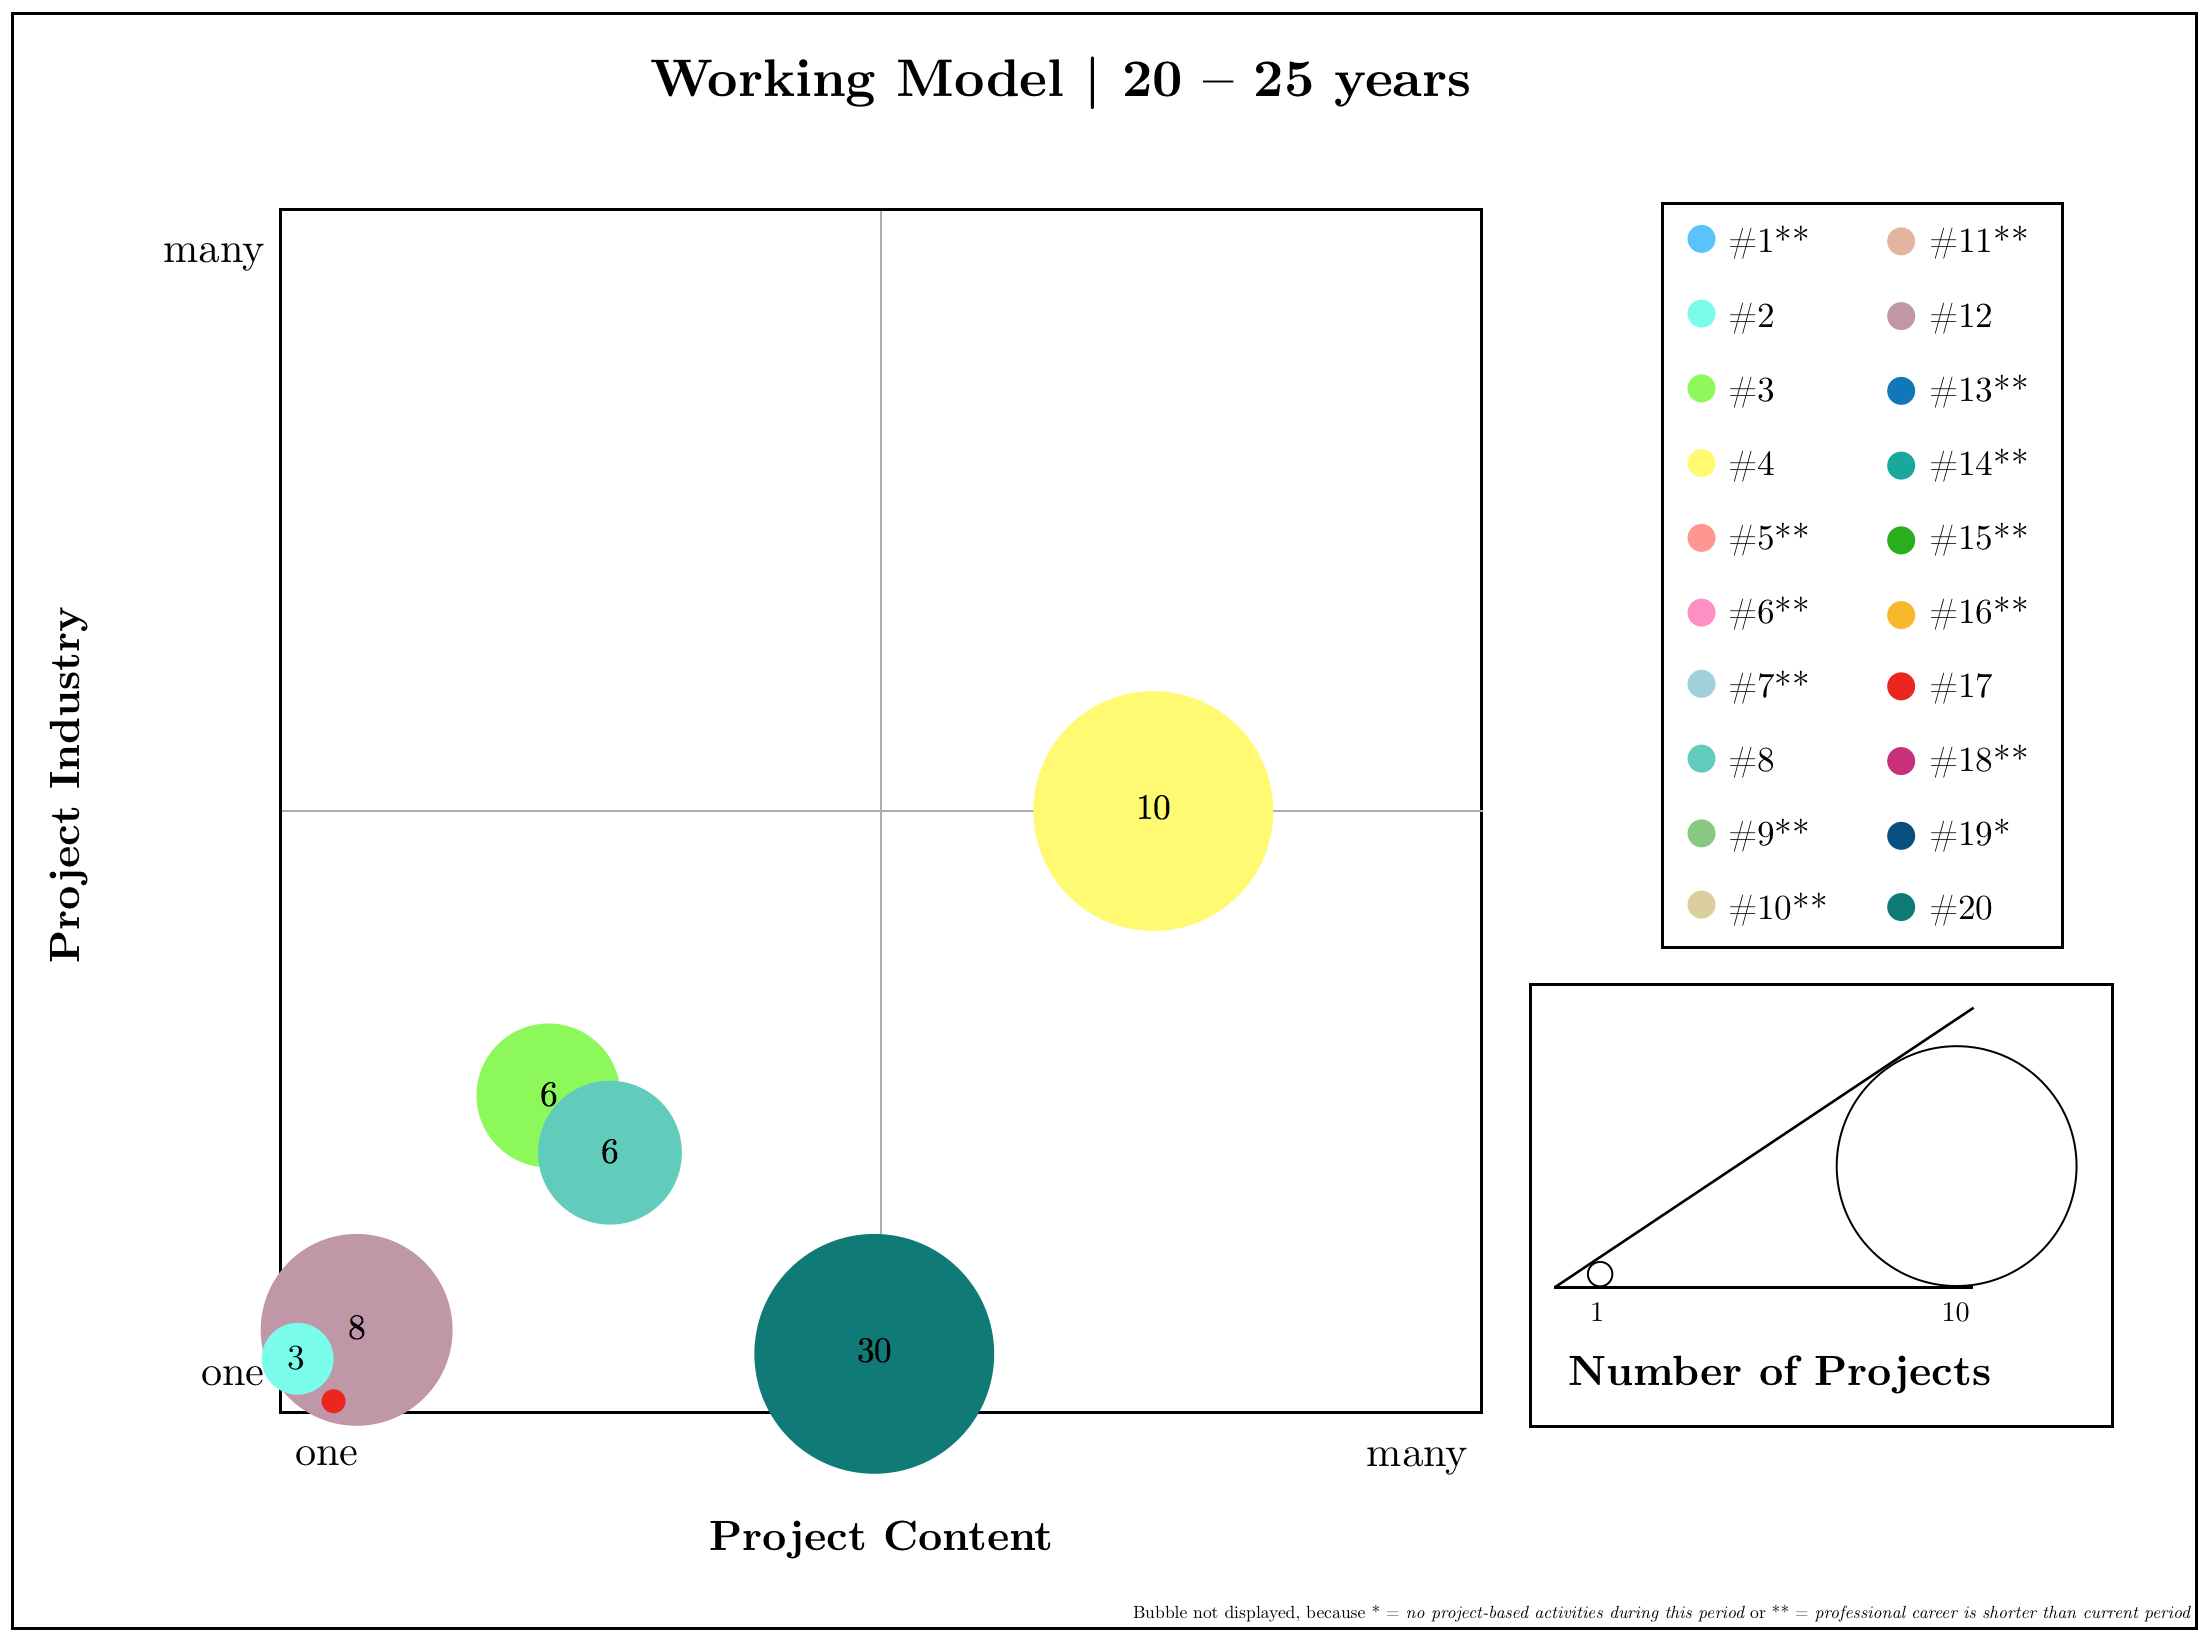
\includegraphics[width=\linewidth]{figures/WM_2025.png}
  \caption[Results of the working model: 20–25 years]{Results of the working model for the \nth{5} career period (20–25 years)}
  \label{fig:WM_2025}
  \endminipage
\end{figure}



%————————————————————–––––––Sub–Subsection–1————––––––––———————————————
%————————————————————Period-specific evaluations———————————————————

\noindent {\bf Period oriented analyses}\\[.1cm]
The first period-oriented analysis figure \ref{fig:analy_CC} (p. \pageref{fig:analy_CC}) analyses the number of company changes per project professional for every time period of his/her career. The basis (total number of project professionals), decreases from period to period as the majority of the interviewees have a professional experience shorter than 25 years, which is also relevant for the following analyses in this subsection (Basis for each period: \nth{1} period: 20 PP; \nth{2} period: 18 PP; \nth{3} period: 15 PP; \nth{4} period: 14 PP; \nth{5} period: 8 PP;). As the this thesis tries to find patterns in the careers of project professionals, this could be a helpful indicator during the analysis. Besides the evaluation of this perspective for the entire sample group, it was also also conducted for each a 'younger' and an 'older' subgroup, which was split according to the  mean age value of 47 years. This additional perspective was taken in order to see if there a significant difference between these two age groups regarding company changes. As the blue line in figure \ref{fig:analy_CC} shows, the number of company changes per project professional decreases over the course of the career, as is falls from 0.60 company changes per PP in the first period to 0.13 in the last one. Furthermore, a difference is evident between the two age groups over the course of their career. In the first two periods the younger subgroup has an elevated level of company changes of 0.75  and 0.67 company changes per PP. However then the rate falls to 0.33 in the \nth{3} period, before rising again drastically to 1 company  change per PP. In contrast, the older subgroup has a lower rate of each time 0.5 in the first two periods, but then increases and outstrips the rate of the other subgroup with a rate of 0.58, before decreasing again drastically in the last two periods to 0.25 and 0.13 company changes per PP.  \\

\begin{figure}[!hbt]
    \captionsetup{font=small}
  \centering
  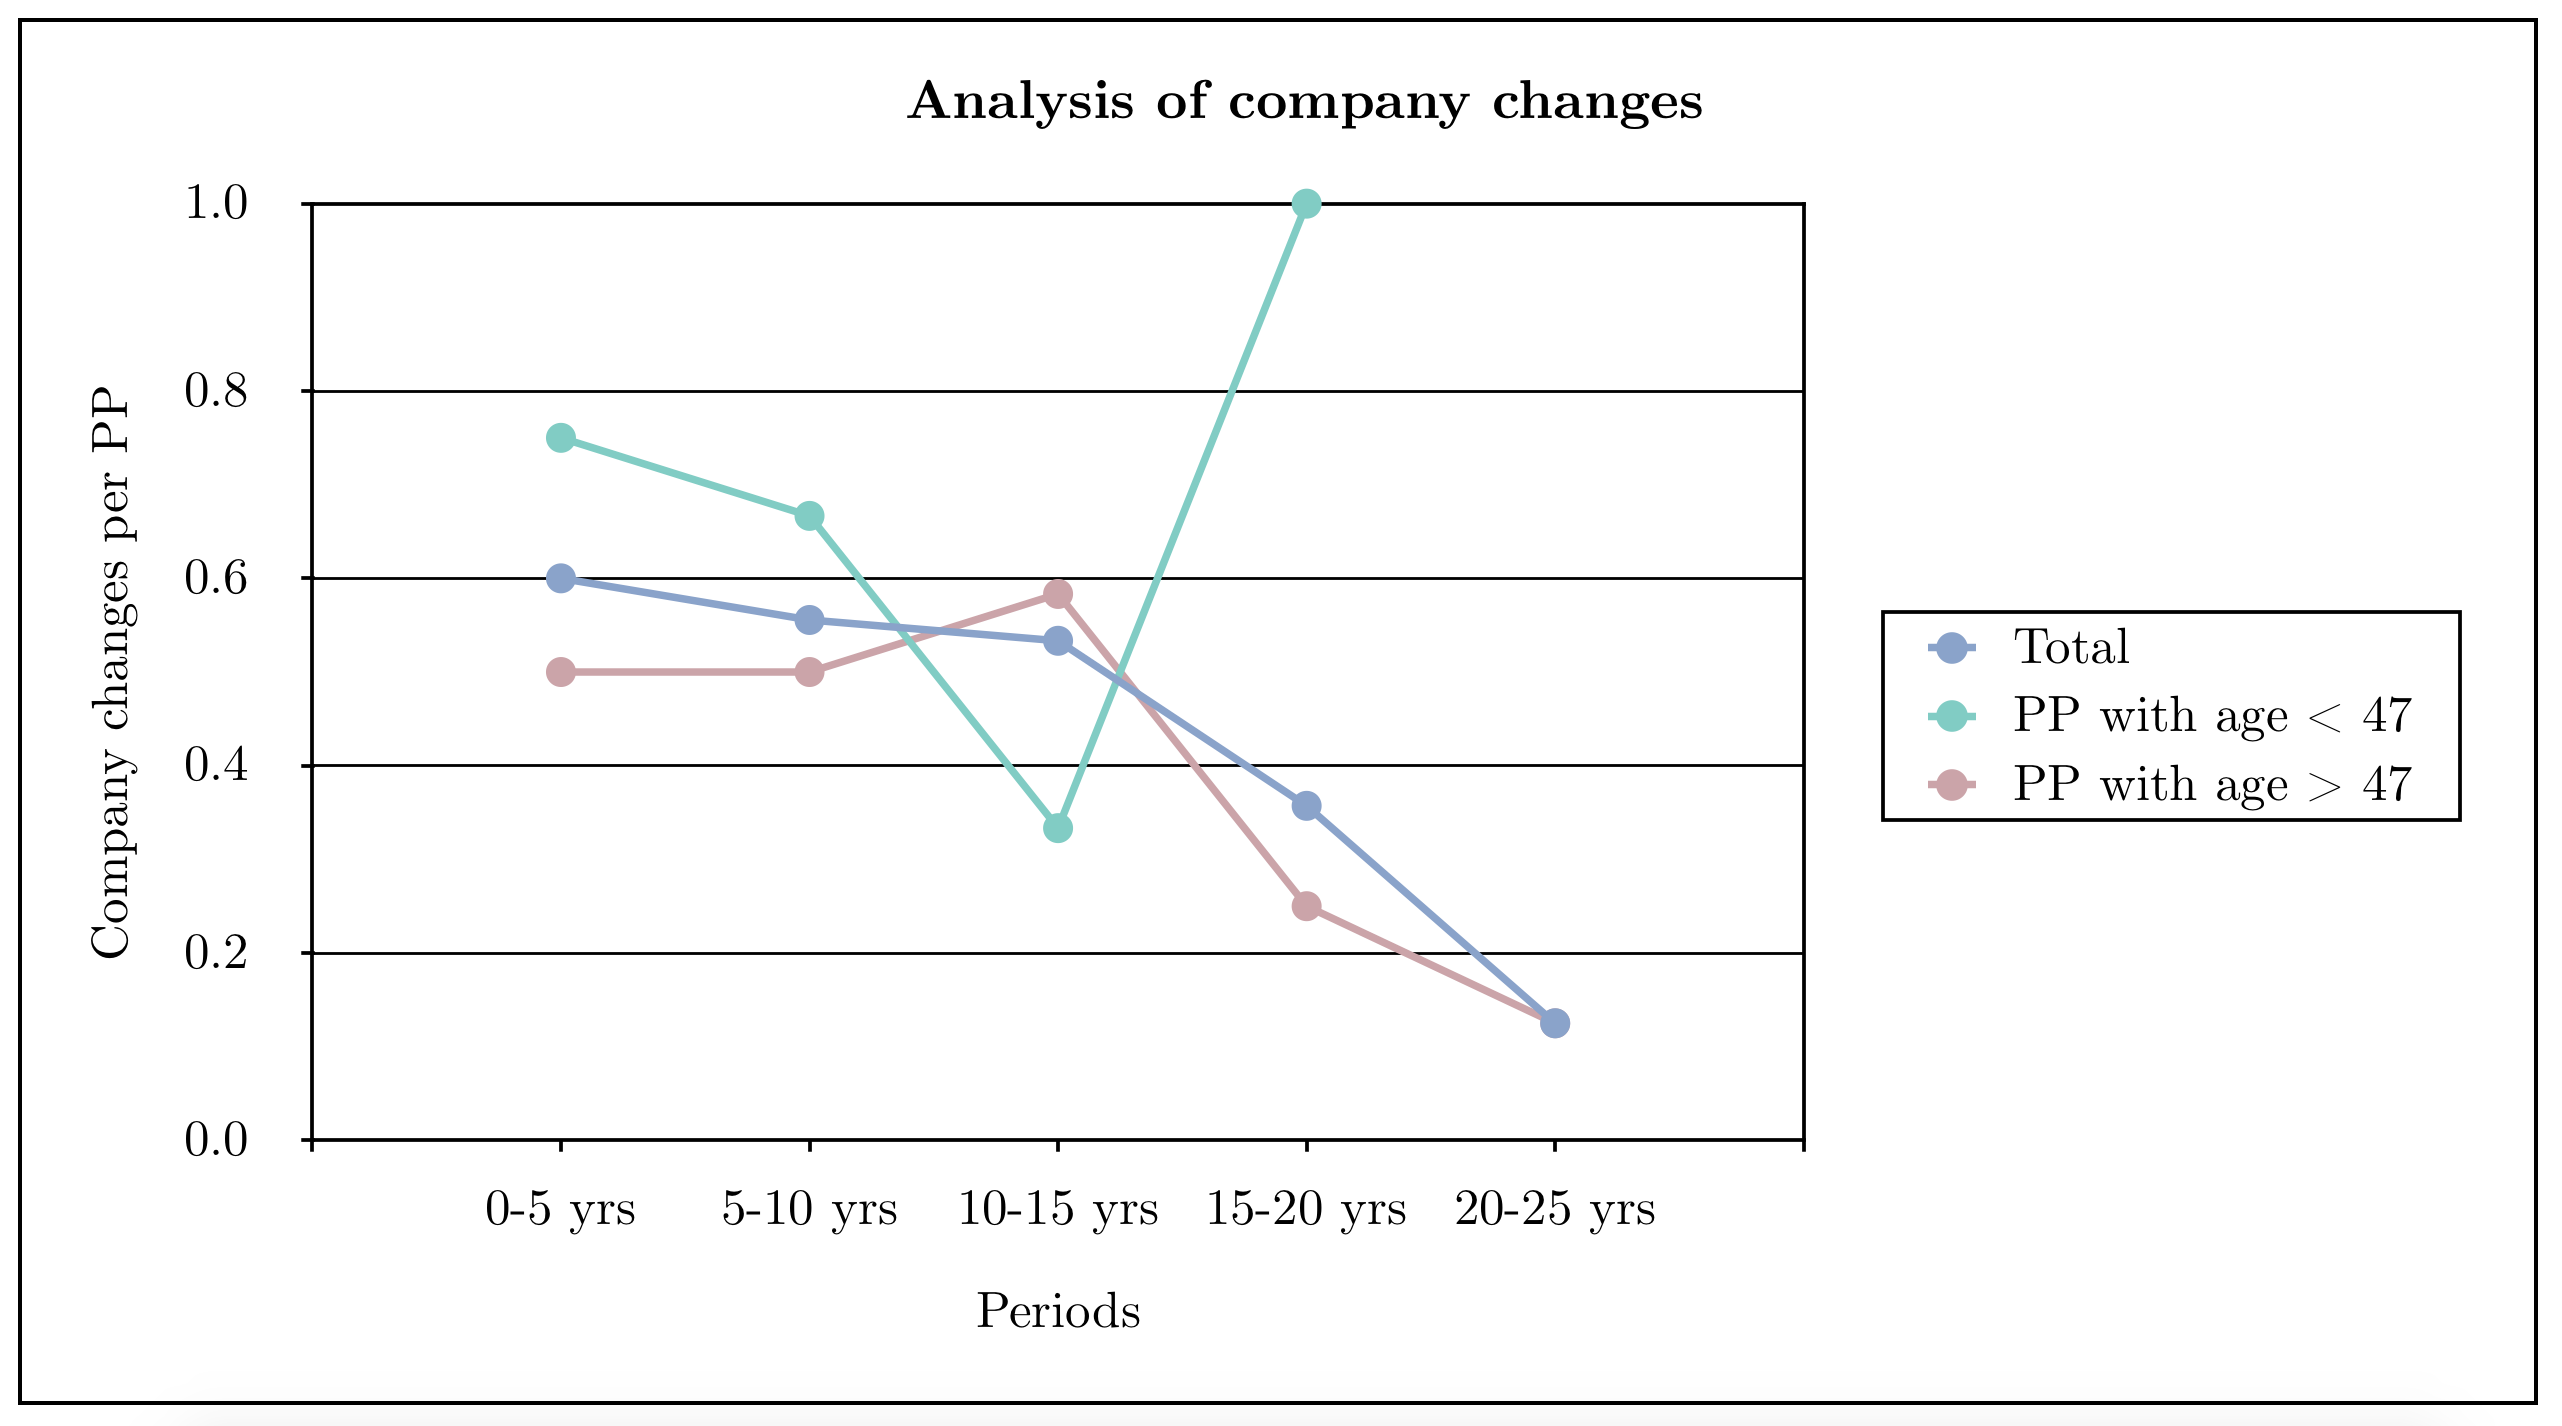
\includegraphics[width=.6\columnwidth]{figures/Analysis_CC.png}
  \caption[Analysis of company changes]{Analysis of company changes per candidate for each career period. The results are shown not only for the entire sample, but also the younger and older half of it (divided by the mean age 47).}
  \label{fig:analy_CC}
\end{figure}


Figure \ref{fig:analy_PCI} (p. \pageref{fig:analy_PCI}) and figure \ref{fig:analy_NP} (p. \pageref{fig:analy_NP}) take a similar perspective as they both evaluate two or one, respectively, of the three dimensions of the main working model and set them into relation to active project professionals and each of the periods. Hereof, active project professionals refer to those those project professionals, who did project-based work in the corresponding period.

The first of the two figures, figure \ref{fig:analy_PCI}, depicts the results of the evaluation of in how many project contents and industries the active project professionals worked in each of the periods on average. Thereby it gives an insight into the distribution of the two indicators over the project professional's career. The results show respectively  project industries that in the \nth{1} career period projects in the most project industries are conducted (2 per active PP). In the \nth{4} period an almost as high value is reached with 1.92 per active PP. In the other three time periods values of between 1.57 and 1.62 project industries per active PP are evident. With respect to the second dimension depicted in figure \ref{fig:analy_PCI}, project contents, it showcases a lower number of project contents per active PP of 1.74 in the first period. In the following two periods the average number of project contents worked in overtakes the avergae number of project industries, with values of 1.87 and 1.92, before falling to the lowest value of the entire depicted time span  of 1.69 per active PP. In the last period of their career an average of 2 project contents per active PP were worked in.  \\

\begin{figure}[!hbt]
    \captionsetup{font=small}
  \centering
  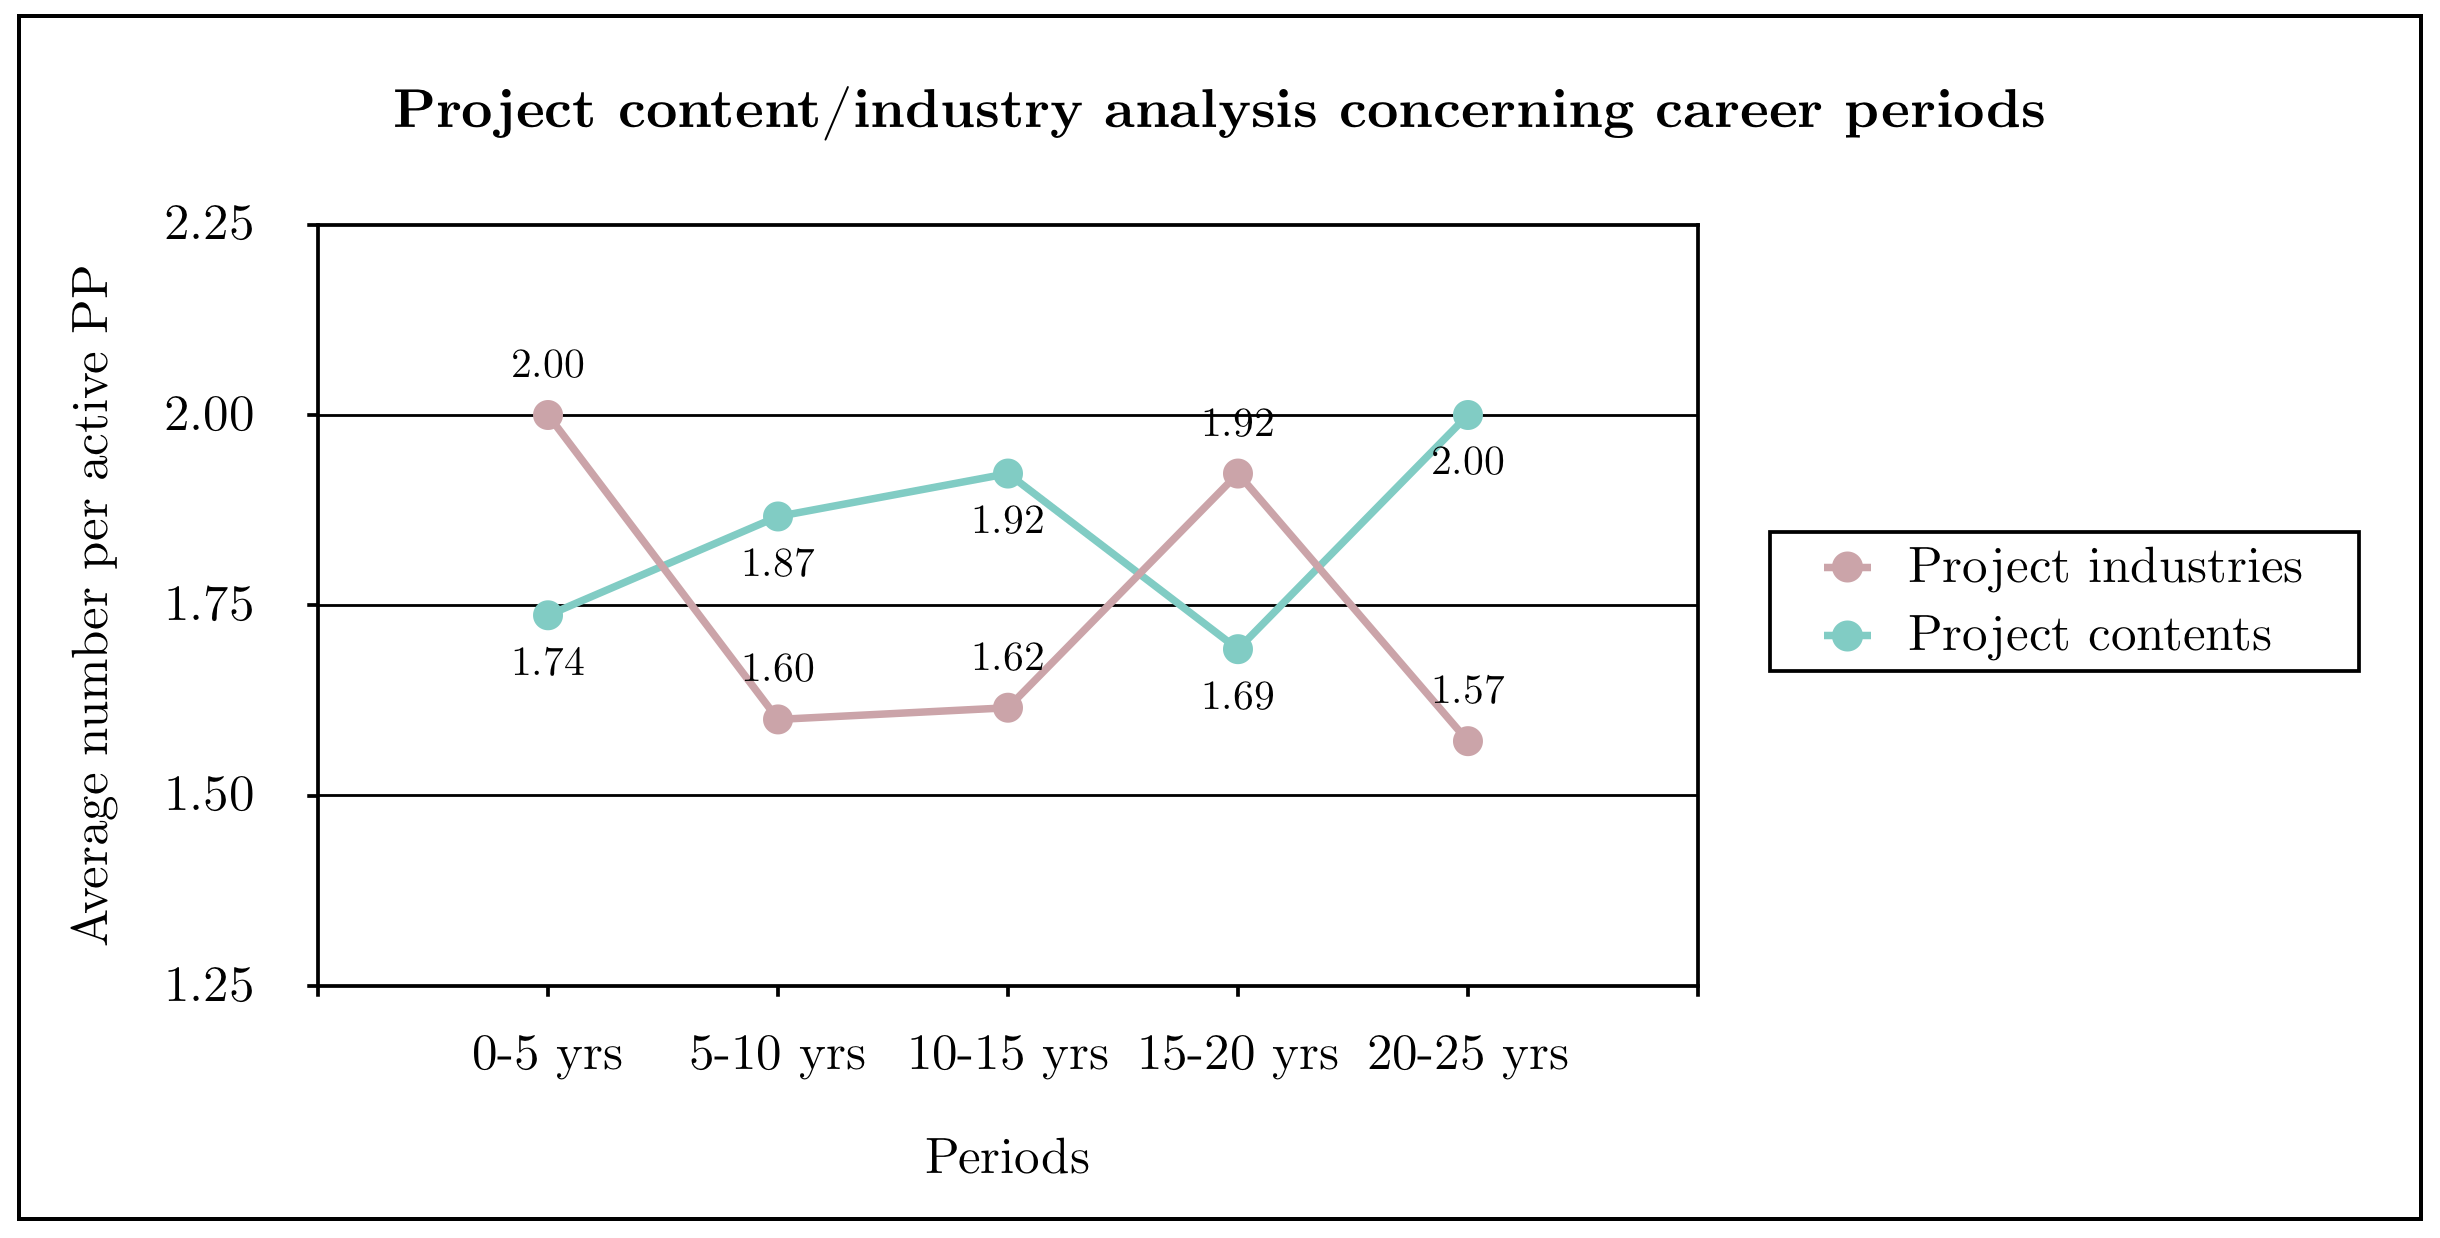
\includegraphics[width=.6\columnwidth]{figures/Analysis_PCI.png}
  \caption[Analysis of project contents and industries respectively the PP's career]{Analysis of the average number of project contents and industries respectively each period of the project professional's career}
  \label{fig:analy_PCI}
\end{figure}

The second figure, figure \ref{fig:analy_NP}, analyses the average number of projects conducted per active project professional for each of the five career periods. It helps, as the before presented figure, to get a feeling for how the average number of projects conducted is distributed over the sample group's career. The results show that the number of projects conducted is elevated (7.74) in the \nth{1} period, in comparison to the \nth{2} and \nth{3} period, where the value is relatively stable at about 1.6 projects contents per active PP. However, in the last two terms it rises drastically to 7.62 and 9.14 per active PP, respectively.\\


\begin{figure}[!hbt]
    \captionsetup{font=small}
  \centering
  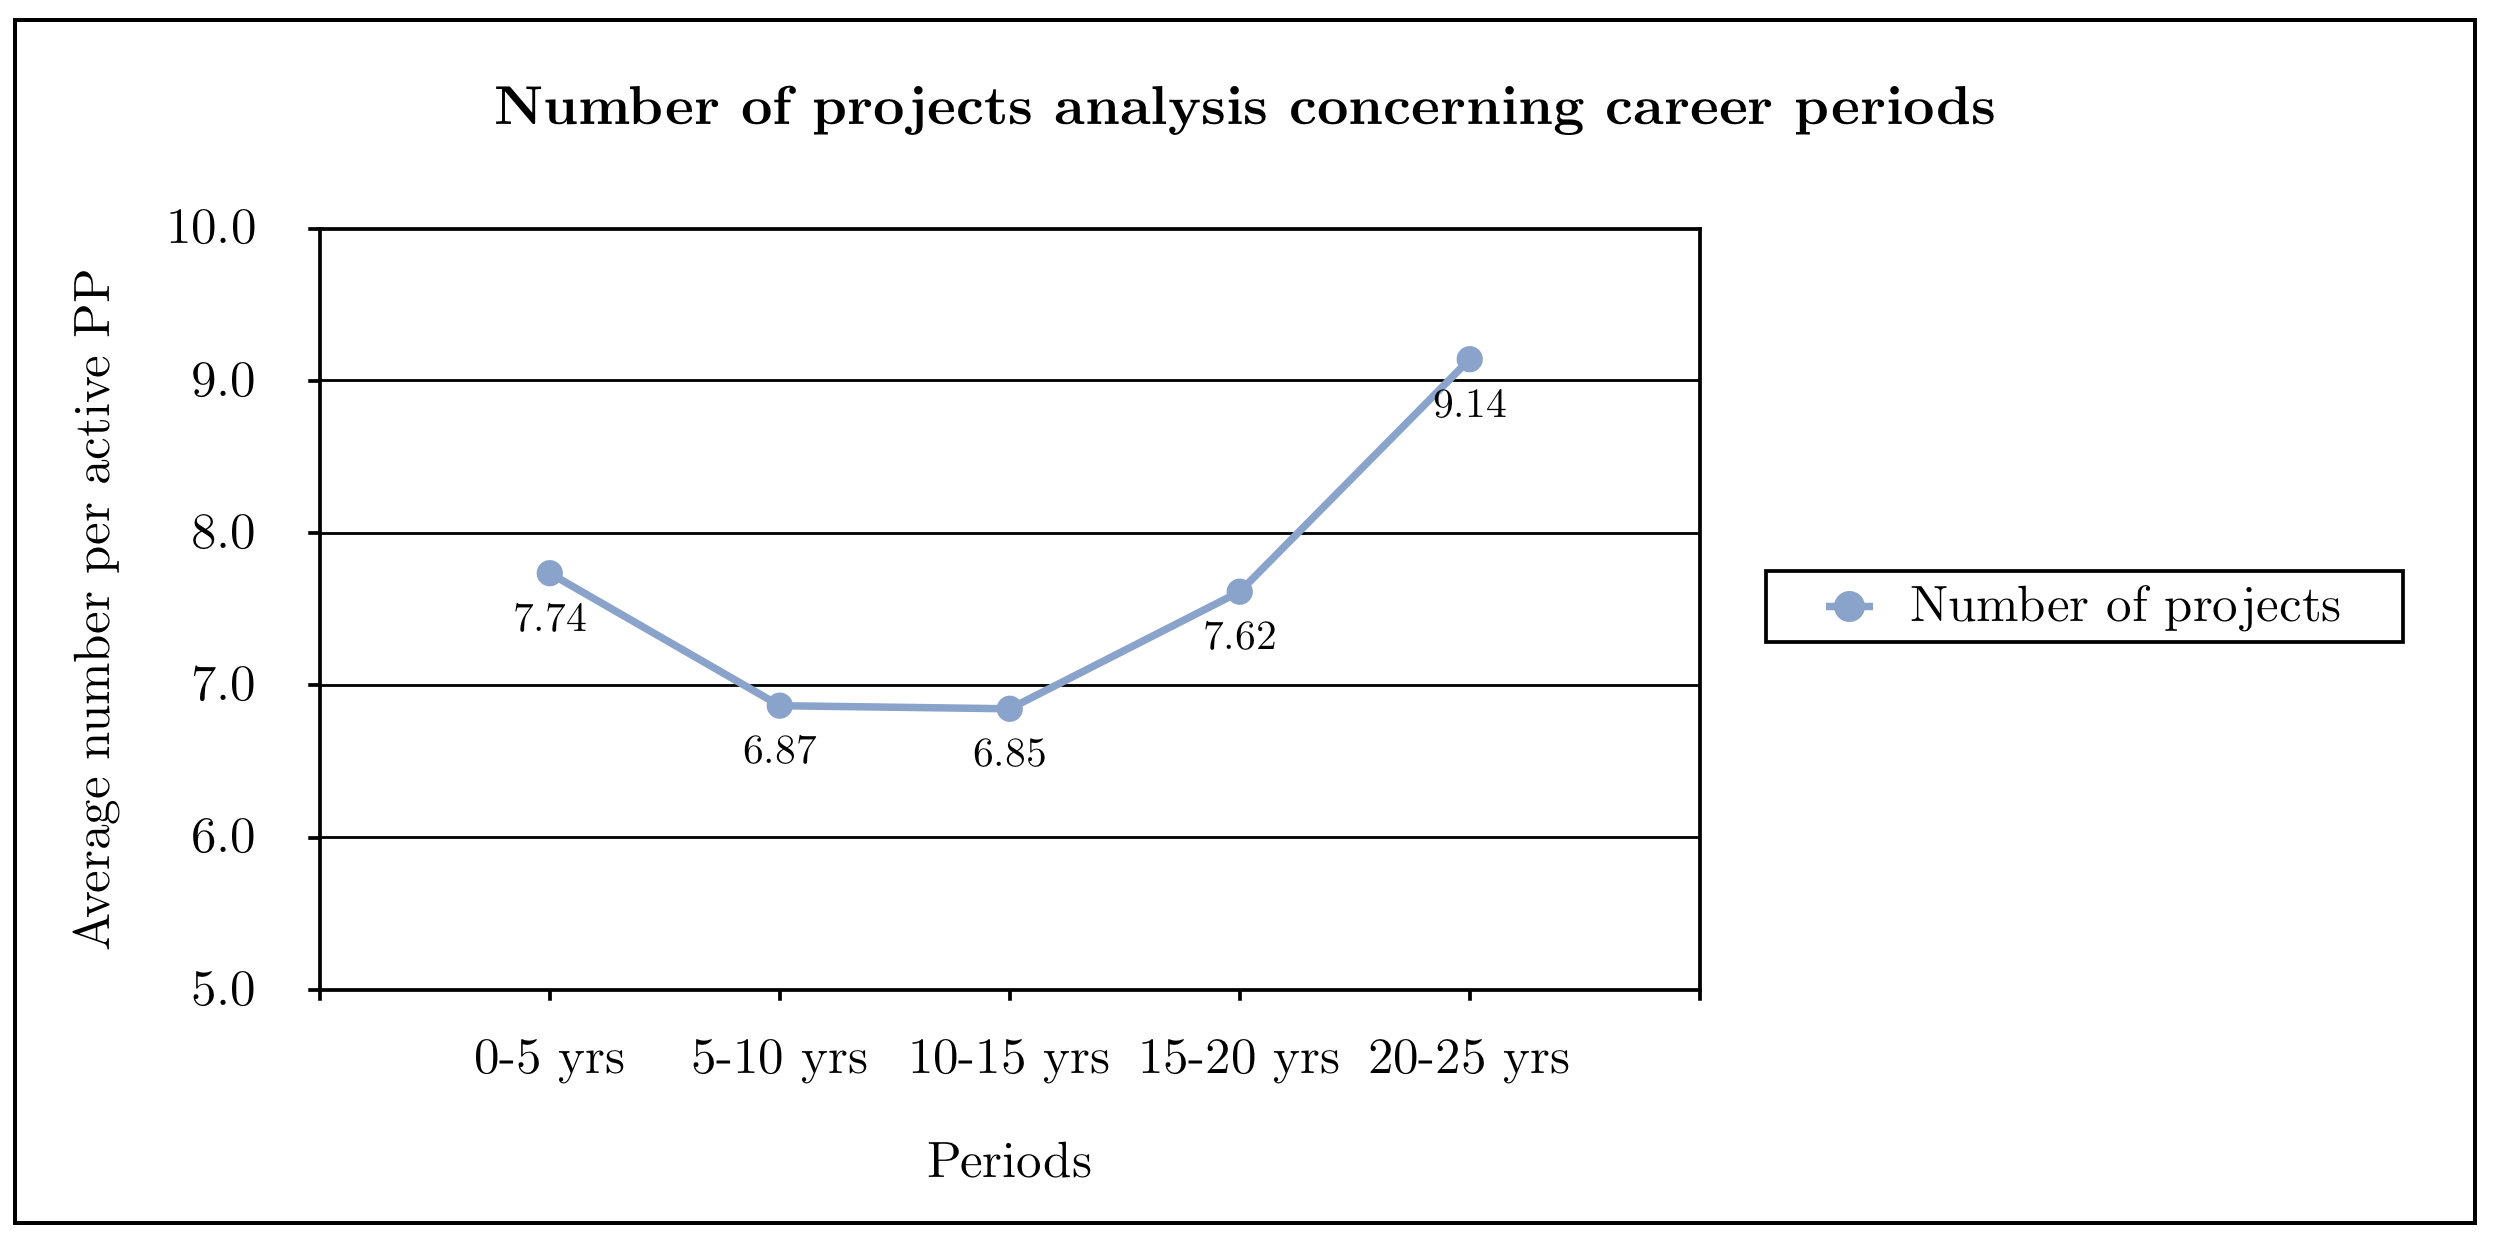
\includegraphics[width=.6\columnwidth]{figures/Analysis_NP.png}
  \caption[Analysis of the number of projects respectively the PP's career]{Analysis of the average number of projects respectively each period of the project professional's career.}
  \label{fig:analy_NP}
\end{figure}



%————————————————Project–content/industry–evaluations———————————————

\noindent {\bf Project oriented analyses}\\[.1cm]
The analyses presented in this part are aimed at examining which project contents and industries were conducted the most in the total 67 five year-periods and if these correspond the distribution of industry backgrounds of the interviewees.

The first table, table \ref{tab:studycont} 
(p. \pageref{tab:studycont}), illustrates all possible project contents and the corresponding quantity they were identified in the data sets. The results show that the most found project contents were \textit{IT projects} (44), \textit{Organisational development projects} (24), \textit{Investment projects} (15), \textit{Strategy projects} (12) and \textit{Feasibility studies, Planning projects} (11). Furthermore, it can be derived that all of the 11 different project contents were at least found once.\\



\begin{table}[!hbt]
\centering
\captionsetup{font=small}
\footnotesize
    \begin{tabular}{|l|l|}
    \hline
    Project Content                                             & Quantity \\ \hline
    IT projects                                                 & 44       \\
    Organisational development projects                         & 24       \\
    Investment projects (construction, plant engineering, etc.) & 15       \\
    Strategy projects                                           & 12       \\
    Feasibility studies, planning projects                      & 11       \\
    Marketing projects, event projects                          & 6        \\
    Research projects, product development projects             & 5        \\
    Company participation projects                              & 2        \\
    Maintenance projects, large-scale repairs                   & 2        \\
    Company formation and acquisition projects                  & 1        \\
    Acquisition projects, tender projects                       & 1       \\ \hline
    \end{tabular}
    \caption[Total number of each project content in sample group]{Total number of each project content in the sample group.}
    \label{tab:studycont}
\end{table}


Table \ref{tab:studyindu} on page \pageref{tab:studyindu} takes the perspective, but for the project industries. It shows that projects in 18 different industries were worked in by the project professionals of the sample group. The ones which were found the most are \textit{Infrastructure} (17), \textit{Information systems} (17), \textit{Health and social services} (13) and \textit{Telecommunications} (12).\\

\begin{table}[!hbt]
\centering
\captionsetup{font=small}
\footnotesize
    \begin{tabular}{|l|l|}
    \hline
    Project Industry                  & Quantity \\ \hline
    Infrastructure                    & 17       \\
    Information systems               & 17       \\
    Health and social services        & 13       \\
    Telecommunications                & 12       \\
    Environmental, waste, sewerage    & 8        \\
    Financial services and insurance  & 7        \\
    Manufacturing                     & 7        \\
    Business and consulting           & 6        \\
    Education and training            & 6        \\
    Process plant                     & 5        \\
    Information technology            & 5        \\
    Electronics                       & 5        \\
    Aerospace                         & 3        \\
    Arts, entertainment, broadcasting & 3        \\
    E-commerce                        & 2        \\
    International development         & 1        \\
    Chemicals and pharmaceuticals     & 1        \\
    Food                              & 1        \\
    Building                          & 0        \\
    Defence                           & 0        \\
    Recreation and sport              & 0        \\
    Automotive                        & 0        \\
    Research and development          & 0     \\ \hline  
    \end{tabular}
    \caption[Total number of each project industry in sample group]{Total number of each project industry in the sample group.}
    \label{tab:studyindu}
\end{table}




%————————————————————Candidate-specific–evaluations———————————————————

\noindent {\bf Individual oriented analyses}\\[.1cm]
The last category of the conducted accompanying analyses takes the individual perspective of the interviewees and looks at their entire career. In doing so, it evaluates how many distinct project contents and project industries each of the candidates had throughout his/her entire career in total. This analysis was aimed at closing the circle of the in this chapter presented evaluations by presenting the individual perspective and thereby help to explain some of the before-mentioned results. Furthermore, it could help find some pattern for specific industries. However, what has to be considered when looking at these results is the length of the professional experience of each interviewee, as some have more than 25 years, while others under 10 years. As can be seen in figure \ref{fig:analy_cand1} (p. \pageref{fig:analy_cand1}) the total number of different project contents differs vastly between the interview candidates, which are represented by their ID on the bottom. This category is at this point kept relatively short, as the individual perspective is further in-depth analysed in the ensuing section.  \\


\begin{figure}[!hbt]
    \captionsetup{font=small}
  \centering
  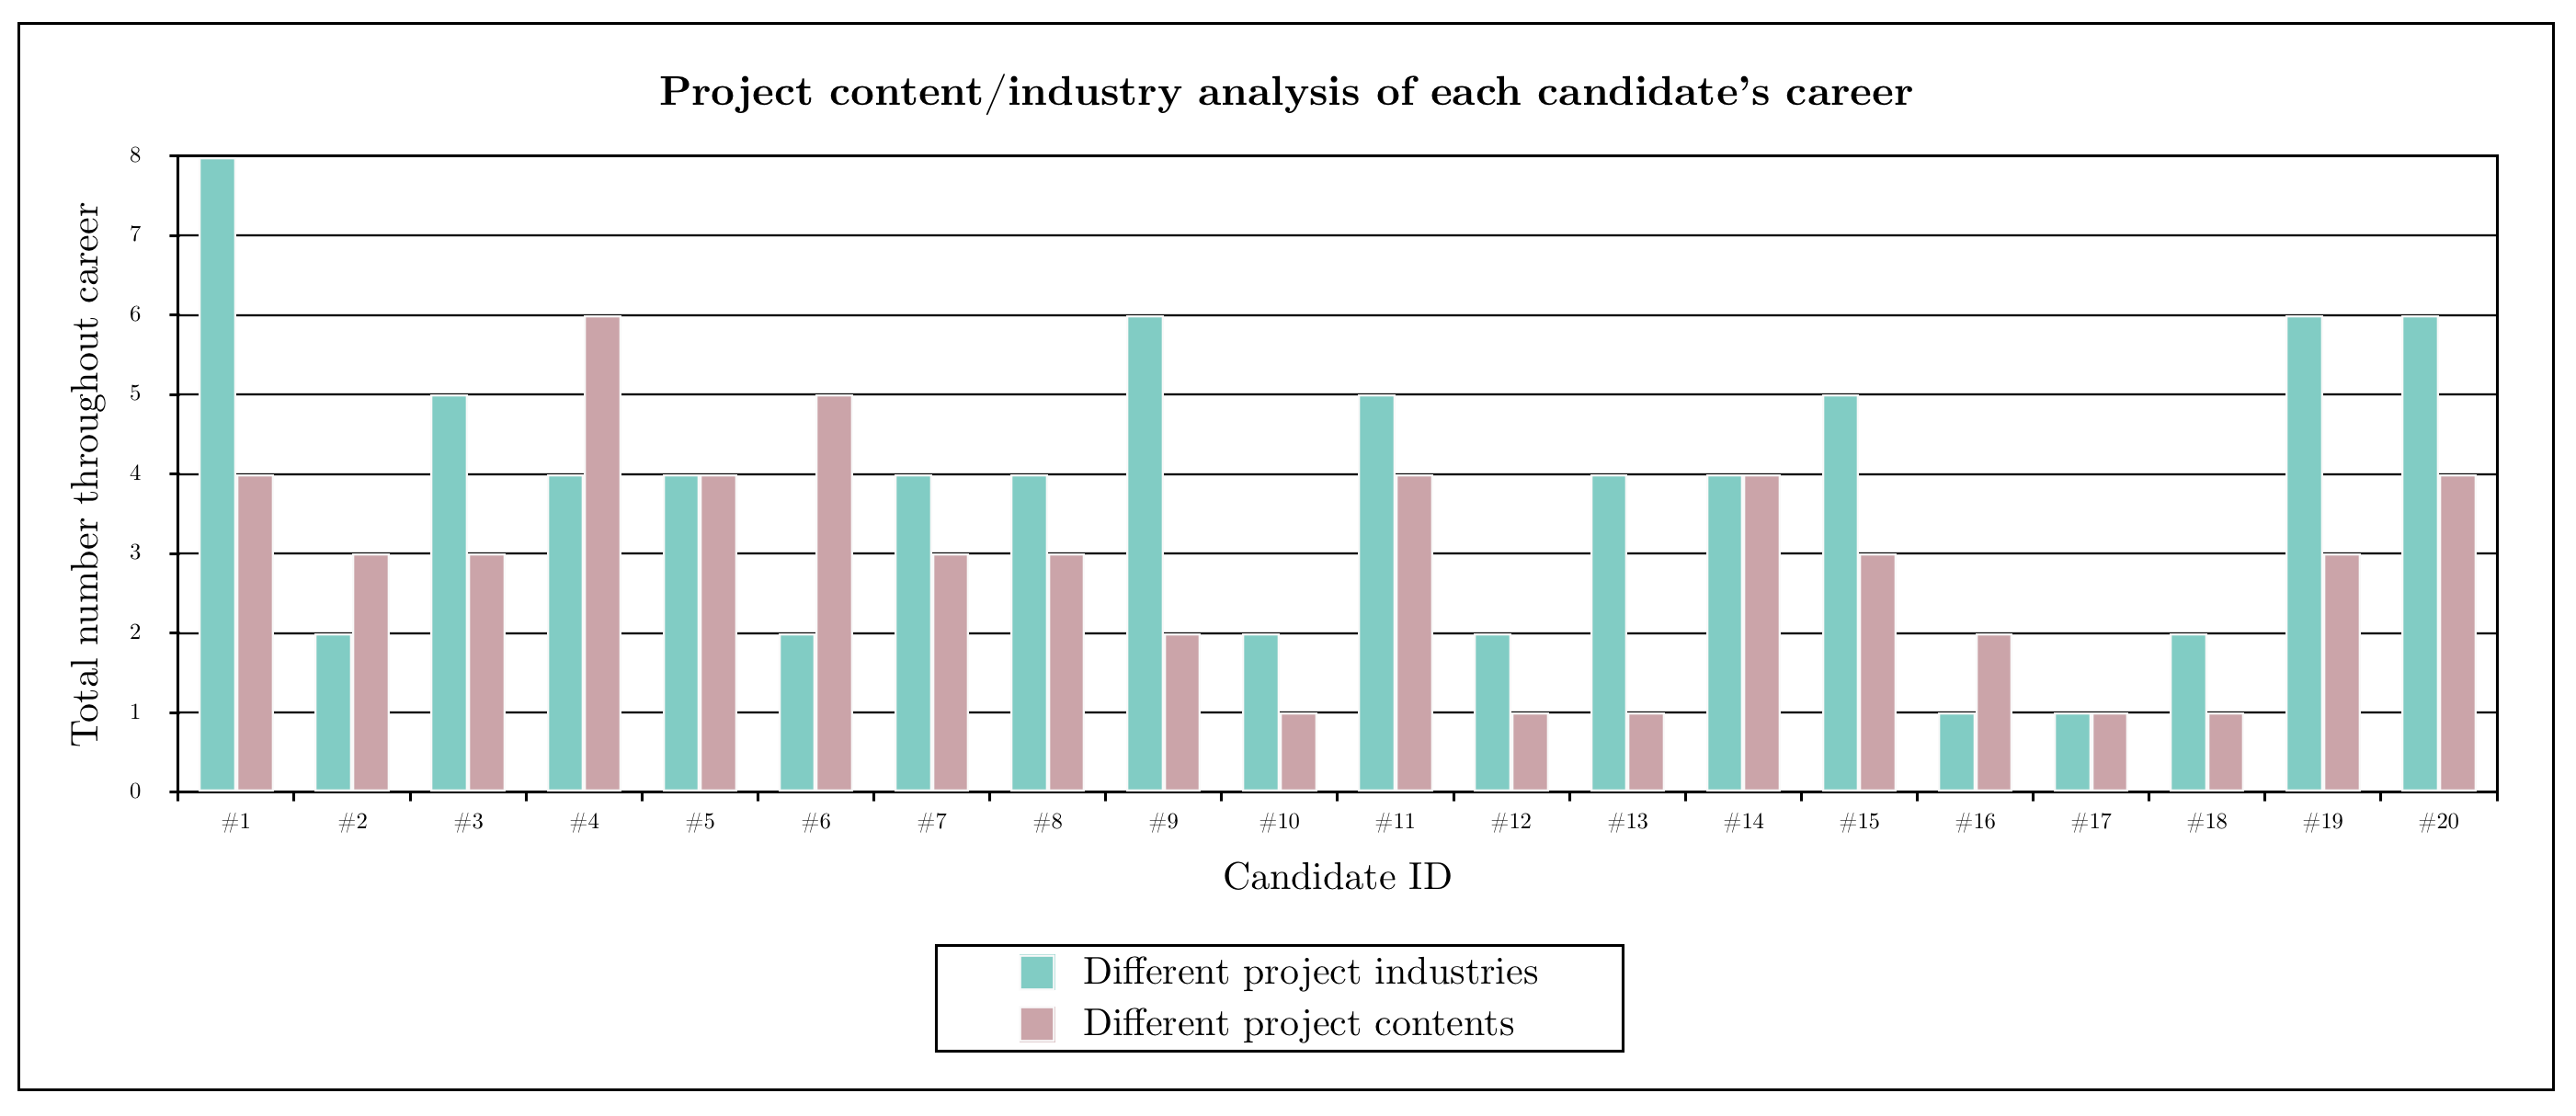
\includegraphics[width=1.0\columnwidth]{figures/Analysis_cand1.png}
  \caption[Analysis of distinct project contents and industries respectively the PP's career]{Analysis of the total number of distinct project contents and industries respectively the entire career of each project professional.}
  \label{fig:analy_cand1}
\end{figure}















%————————————————————–––––––Sub–Subsection–2————––––––––———————————————

\subsubsection{From the career movement model}

After already providing insights from various perspectives into the data sets in the previous subsection, this section takes the findings from the main working model and analyses them for changes or 'movements' during a project professional's career. To do so it uses the career movement model, which was introduced in detail on page \pageref{fig:alternate}f.  \\




%———————————————–––—————The–Individual–perspective—————––———————————

\noindent {\bf The individual career movements}\\[.1cm]
In the first step of this analysis stage, the movements in each project professional's career were visualised using the on page \pageref{sec:cmm}f introduced career movement model, which means for all 20 candidates of the sample group an individual graph was drawn up. These graphs can be seen in figures \ref{fig:CM1} and \ref{fig:CM2} on page \pageref{fig:CM1}f. The graphs are labeled with the candidate's ID on top, so that they can be easily allocated to each interviewee. This first comprehensive visualisation is aimed at facilitating the visual identification of patterns between individuals and furthermore was gives an overview over the careers with respect to project contents and project industries. For example, the graphs of project professionals of the same background, like \#16 and \#17 (both infrastructure industry) can be directly compared and, as can be seen in figure \ref{fig:CM2}, both do mostly projects with the same content and in one project industry. If these can be identified as patterns will be discussed in the following chapter.\\



%———————————————–––—————The–Sector–analysis—————––———————–––––––————

\noindent {\bf The sector analysis}\\[.1cm]
Since a comparative analysis of all the previously presented individual career movement analyses at once would be unfeasible by putting each interviewee's career movements into one graph, a sector classification model was developed, which can be seen in figure \ref{fig:sectors1} on page \pageref{fig:sectors1}. It divides the underlying model into 5 sectors. The sectors form and size was chosen considering not only the non-numeric scaling from one to many of the model, but also the underlying numeric scale, as well as the data sets. Thereby, all points covered by one of the sectors has an similar degree of career differentiation by project industries and project contents. The exact project content (PC) and industry (PI) combinations compromised by each sector are:
\begin{itemize}[noitemsep]
    \item Sector 1: one PC – one PI;
    \item Sector 2: one PC – two PI, two PC – two PI, two PC – one PI;
    \item Sector 3: one PC – three PI, two PC – three PI, three PC – three PI, three PC – two PI, three PC – one PI;
    \item Sector 4: one PC – four PI, two PC – four PI, three PC – four PI, four PC – four PI, four PC – three PI, four PC – two PI, four PC – one PI;
    \item Sector 5: one PC – five PI, two PC – five PI, three PC – five PI, four PC – five PI, five PC – five PI, five PC – four PI, five PC – three PI, five PC – two PI, five PC – one PI;
\end{itemize}
As a result, this enables the analysis and interpretation of the movements between these defined sectors of the entire sample group all at the same time. \\



\begin{figure}[hbt]
    \captionsetup{font=small}
  \centering
  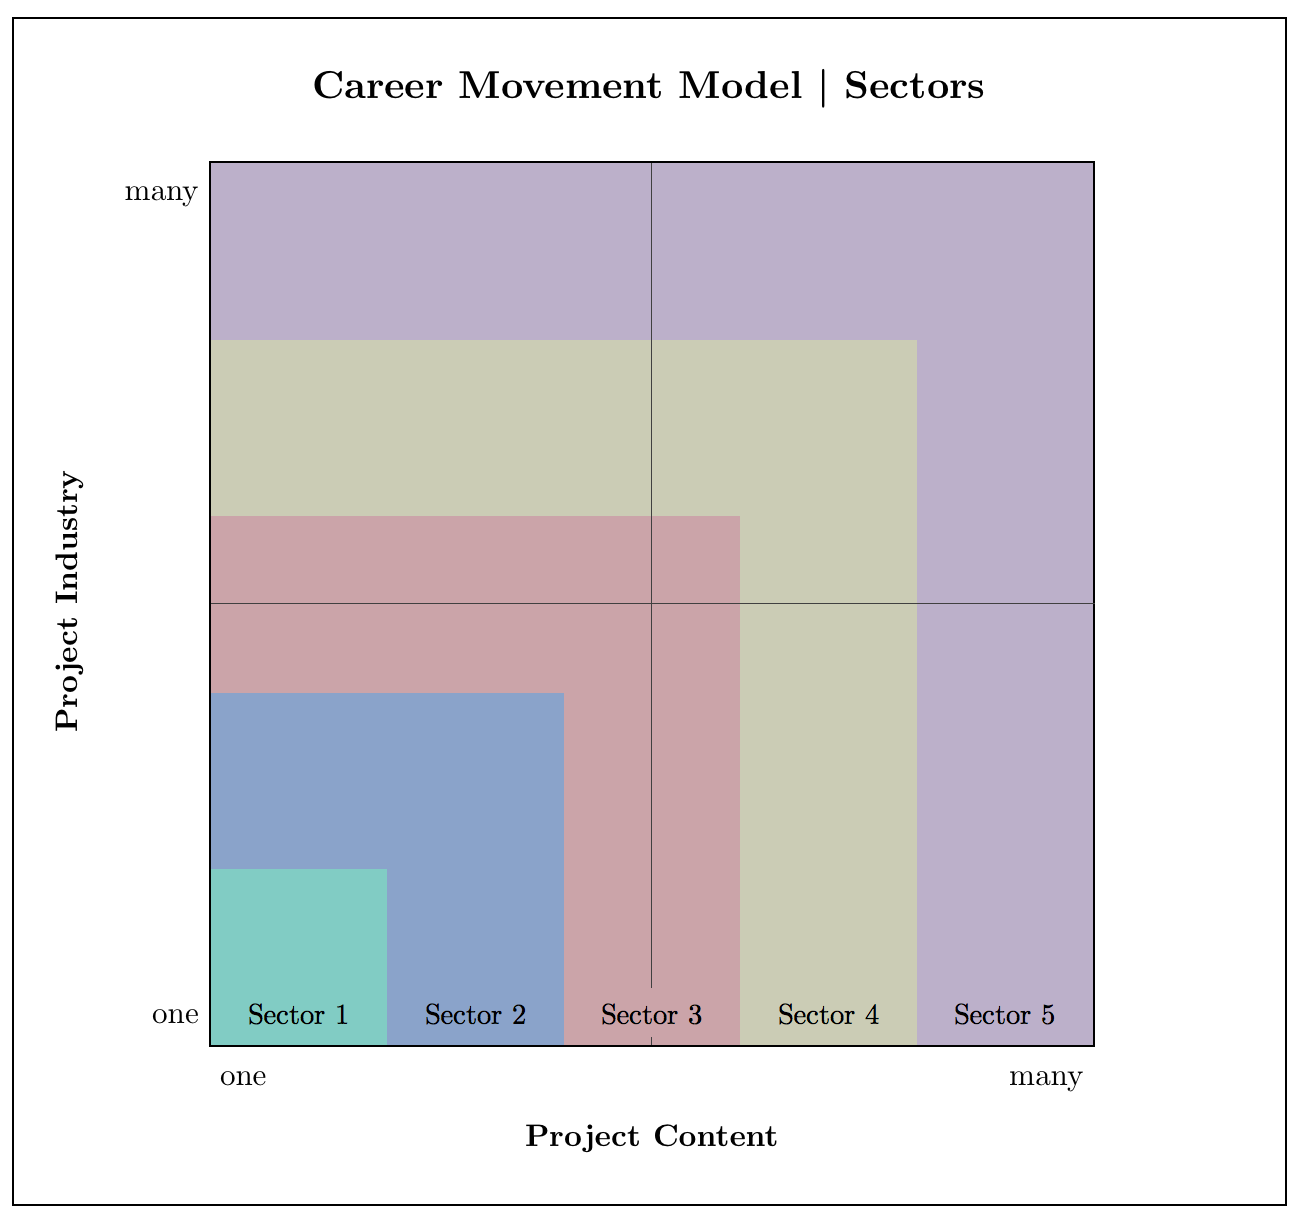
\includegraphics[width=.5\columnwidth]{figures/Analysis_sectors1.png}
  \caption[The sector classifications]{The sector classifications, which are to be used for the career movement model.}
  \label{fig:sectors1}
\end{figure}

\noindent Using this sectorisation, figure \ref{fig:sector2} (p. \pageref{fig:sector2}) shows the outcomes of the conducted sector analysis, which examined how much the bubbles located in a sector made up of the total number of bubbles for each term. Thereby it shows the percentage of project professionals that execute a similar number of different project contents and industries in each step of the career. As can be seen in figure \ref{fig:sector2}, in the first period of their career, 63\% of the project professionals work in project(s) with a maximum of 2 different project contents and/or industries and this trend continues in the second term as the percentage rises to 80\%. However, the first period is also the only one, where some (5\%) project professionals do projects with 5 distinct project contents and or industries. In the third career phase the biggest group (38\%) of project personnel does projects with only one project content and one project industry. The of located in sector 3 is increasing significantly from 7\% in period 2 to 23\%. This movement happens at the cost of sector 2 which falls significantly from 47\% in the \nth{2} term to 23\% in the \nth{3}. This trend further increases, as in the \nth{4} period the majority (46\%) of the sample group conducts projects with 3 project contents and/or industries. In this term none conduct projects in the \nth{4} sector. Sector 1 and 2 project combinations are done by 31\% and 23\%, respectively. In the last career period, however, the share of Sector 3-type project falls drastically to 14\%. Therefore, Sectors 1, 2 and 3 profit and rise again to 43\%, 29\% and 14\%, respectively. \\


\begin{figure}[hbt]
    \captionsetup{font=small}
  \centering
  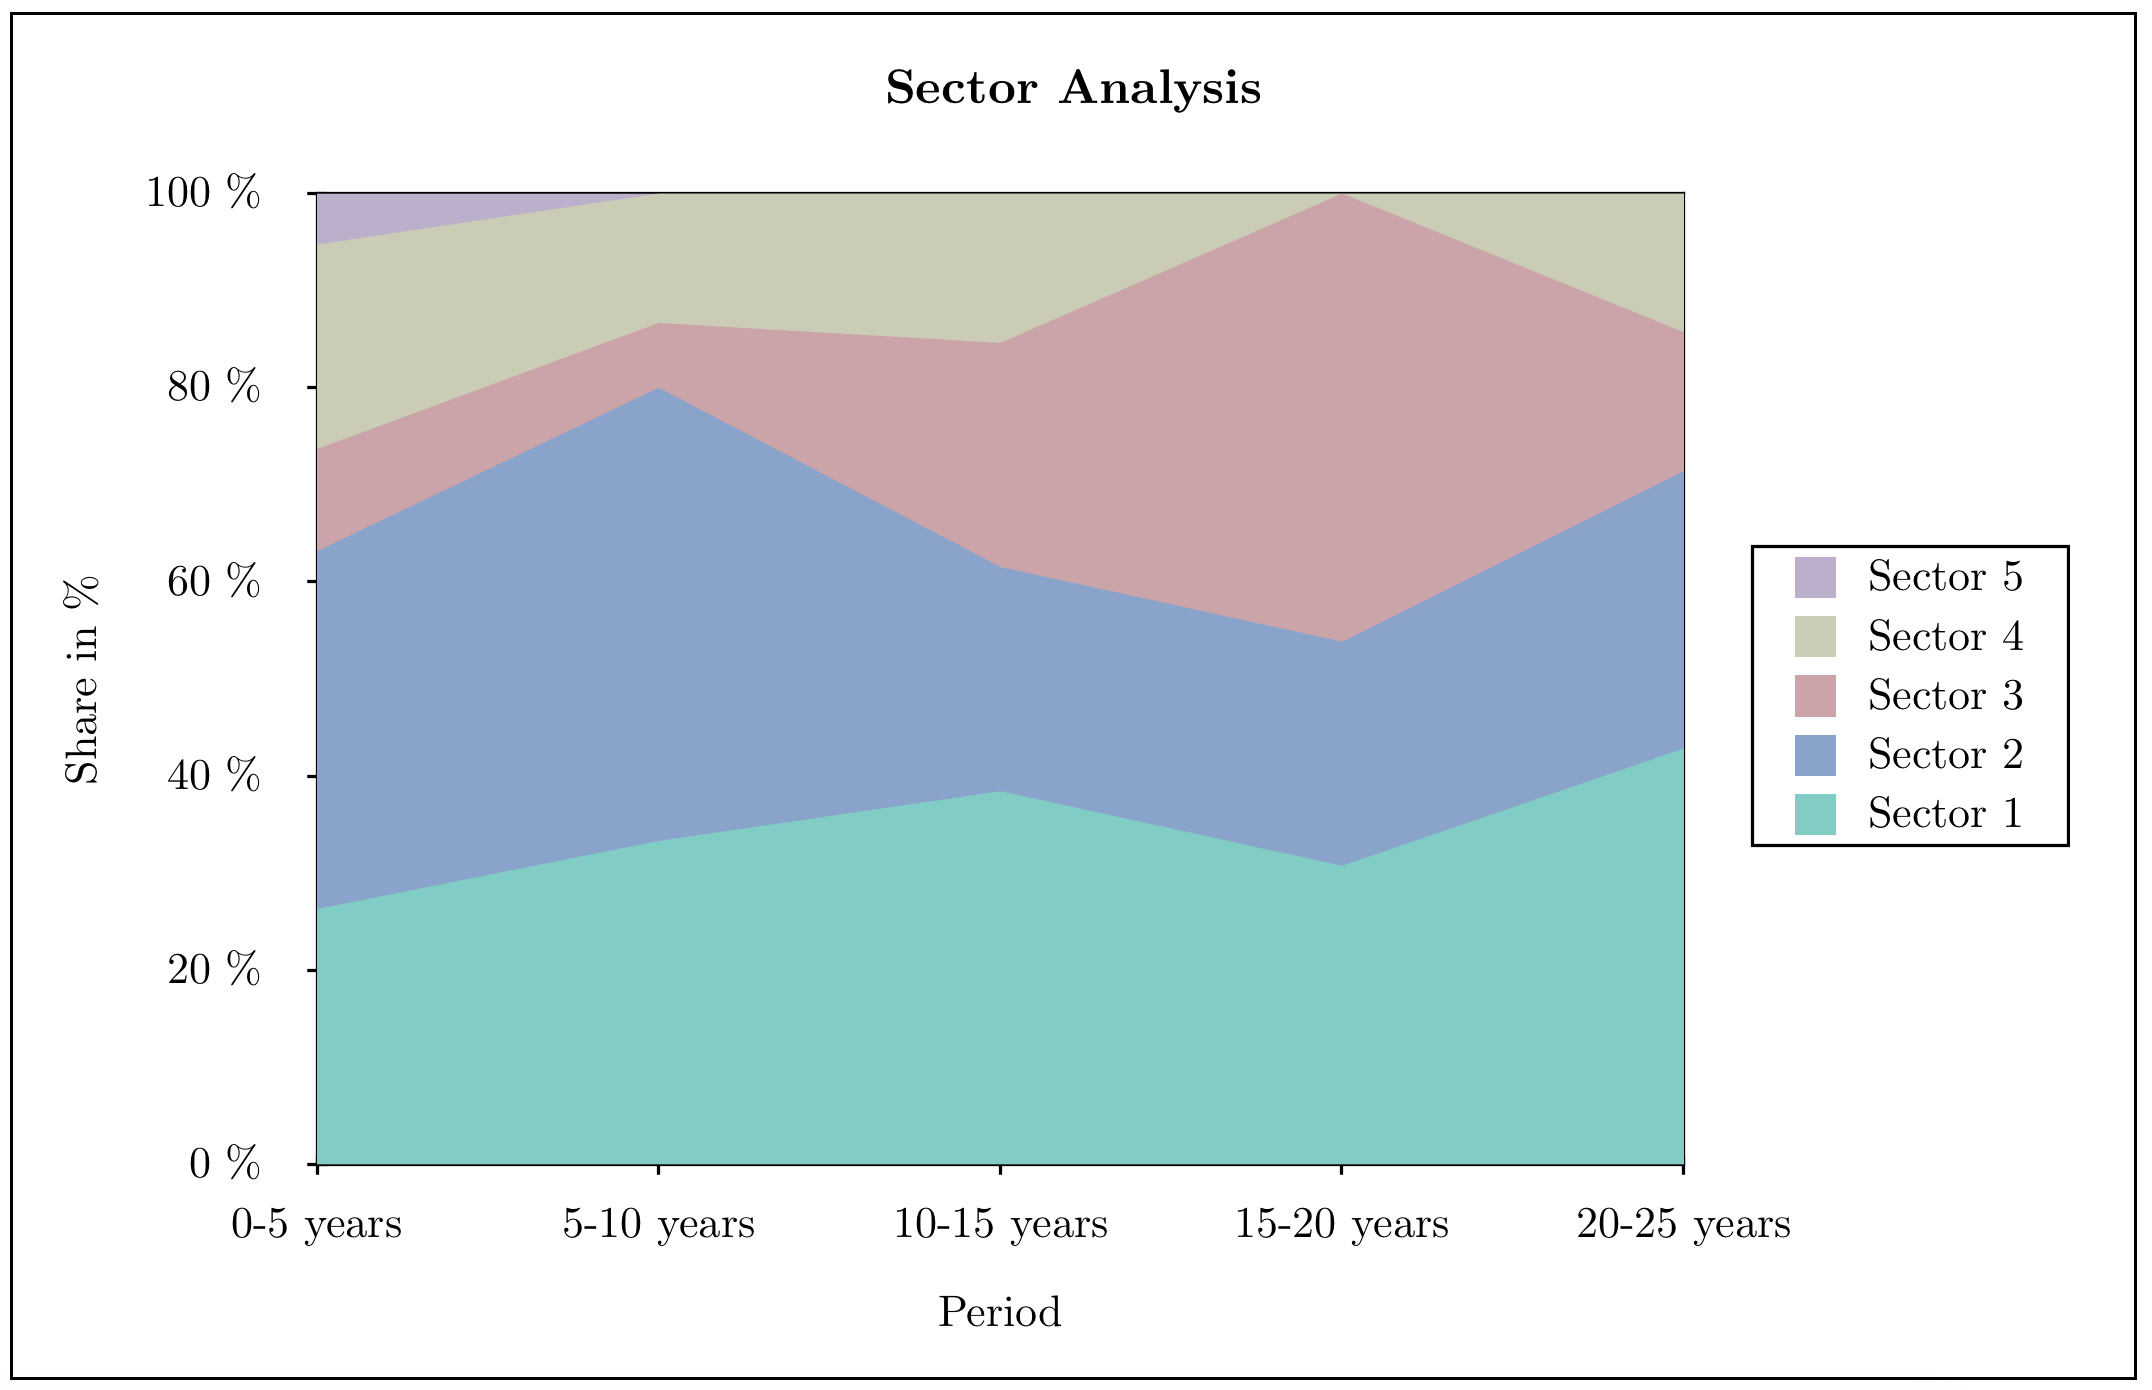
\includegraphics[width=.6\columnwidth]{figures/Analysis_sectors2.png}
  \caption[Results of the sector analysis]{Results of the sector analysis, showing the share of project professionals located in each of the five sector per career period.}
  \label{fig:sector2}
\end{figure}


\subsection{Summary of the study results}
In this chapter, the results of the study, as well as several conducted analyses were presented, which shed a light on the careers of project professionals from perspective. Firstly, it was shown, that the working model fulfils its purpose and delivers analysable results, but also can be applied to the careers of project professional of different backgrounds and form. Furthermore, the visualisation helps to identify pattern and interpret the data, as will be seen in the following chapter. Whether form these obtained findings,  patterns or other assumptions about the careers of project professional can be derived or not will be discussed in the following chapter.  \\

\begin{sidewaysfigure}[!hbt]
    \captionsetup{font=small}
  \centering
  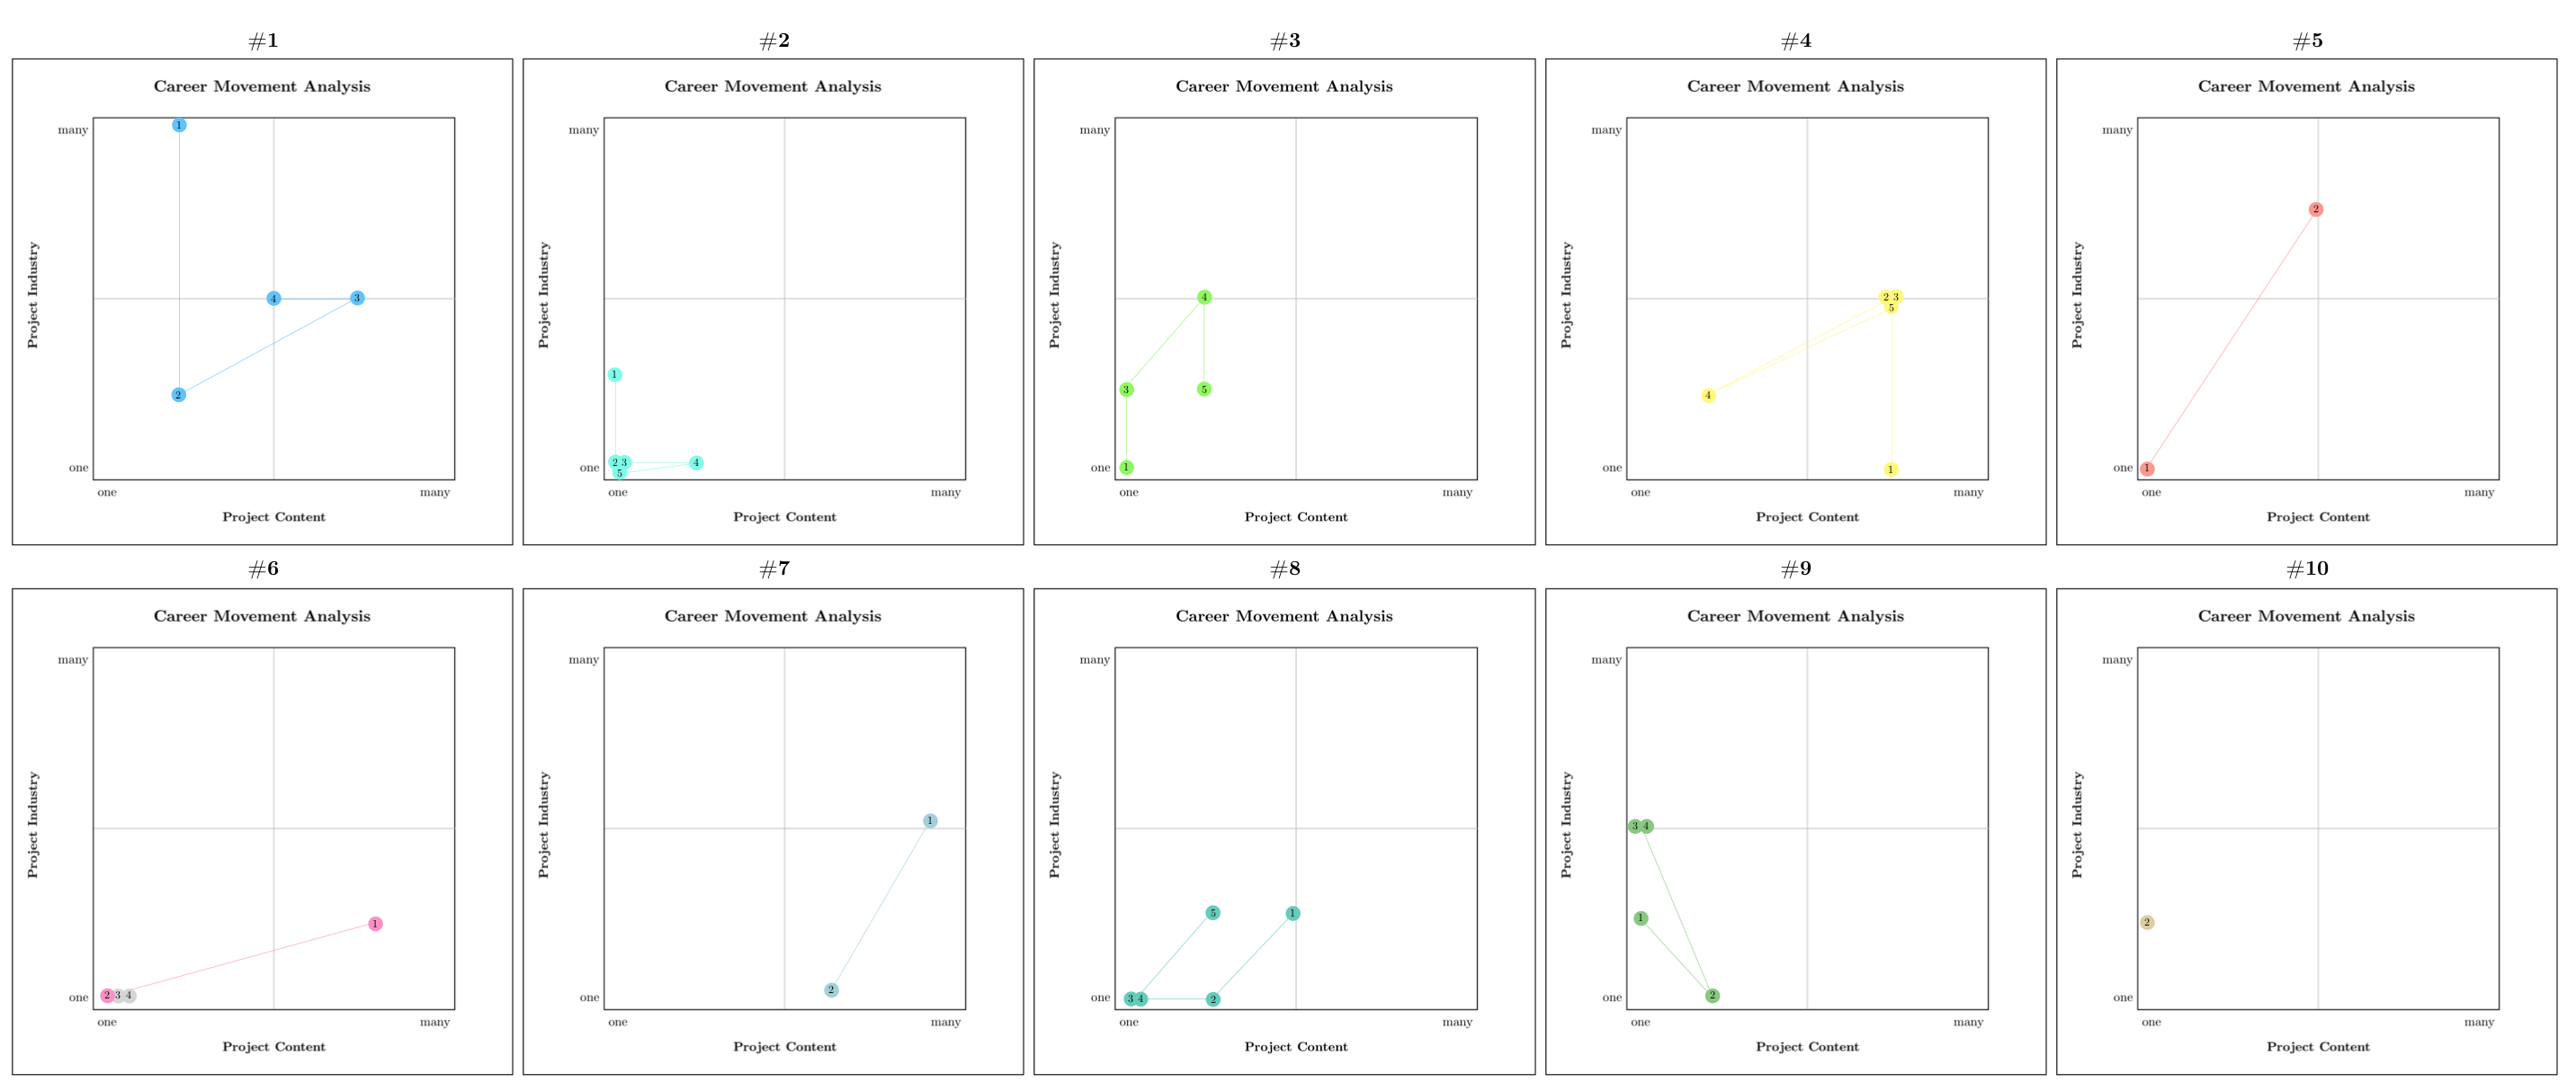
\includegraphics[width=1.0\columnwidth]{figures/Analysis_CM1.png}
  \caption[Results of the career movements model for each individual – Part I]{Results of the career movements model for each individual – Part I}
  \label{fig:CM1}
\end{sidewaysfigure}

\begin{sidewaysfigure}[!hbt]
    \captionsetup{font=small}
  \centering
  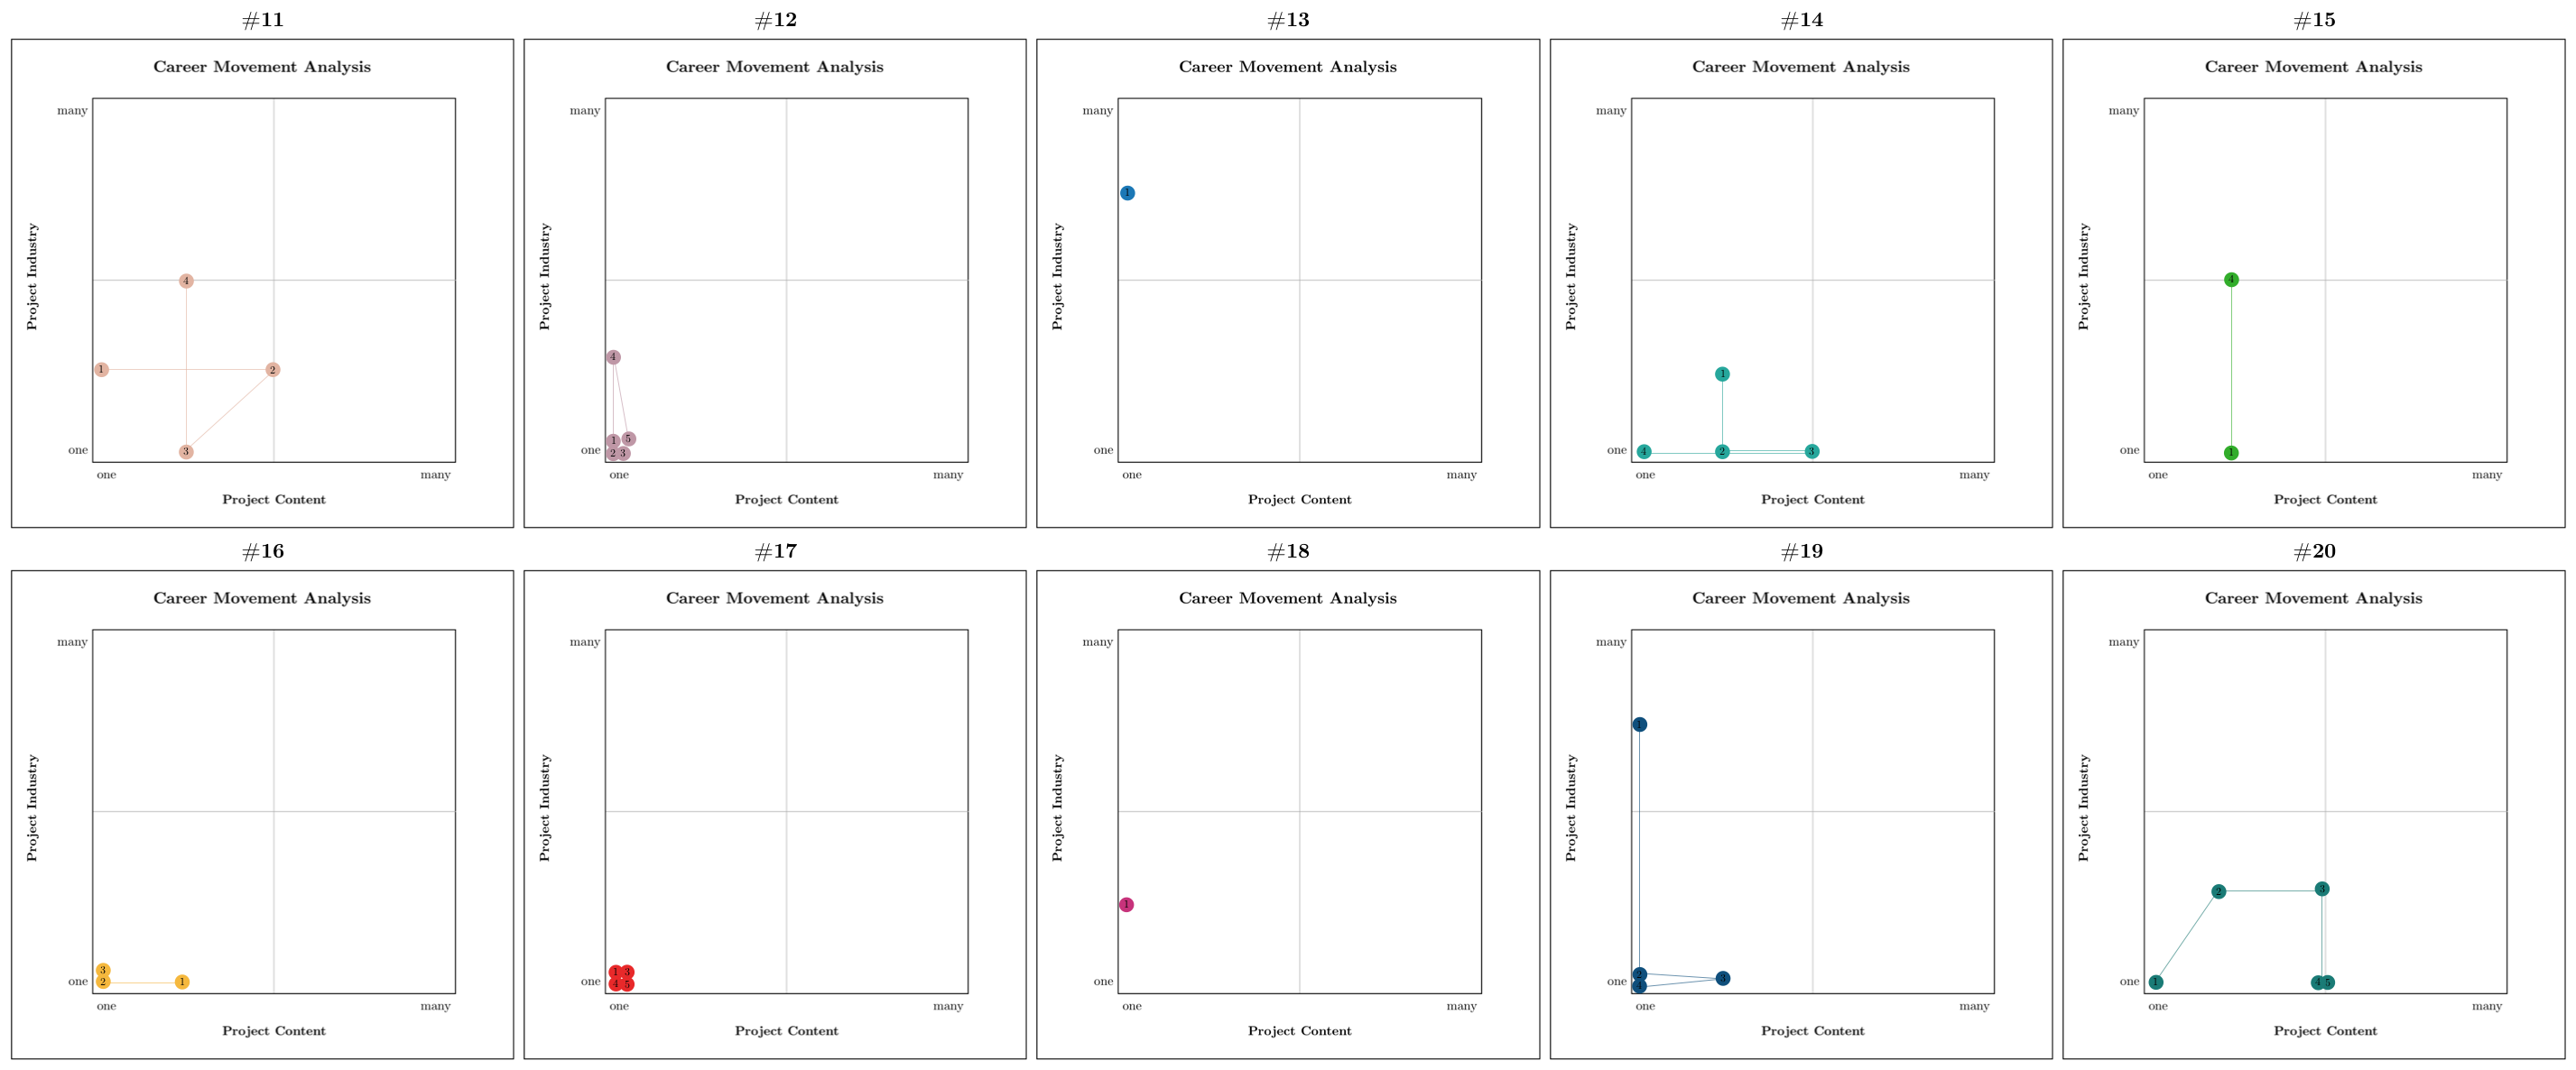
\includegraphics[width=1.0\columnwidth]{figures/Analysis_CM2.png}
  \caption[Results of the career movements model for each individual – Part II]{Results of the career movements model for each individual – Part II}
  \label{fig:CM2}
\end{sidewaysfigure}
\cleardoublepage

\section{Discussion}
\label{sec:discussion}

\blindtext

\begin{figure}[hbt]
\minipage[t]{0.48\textwidth}
  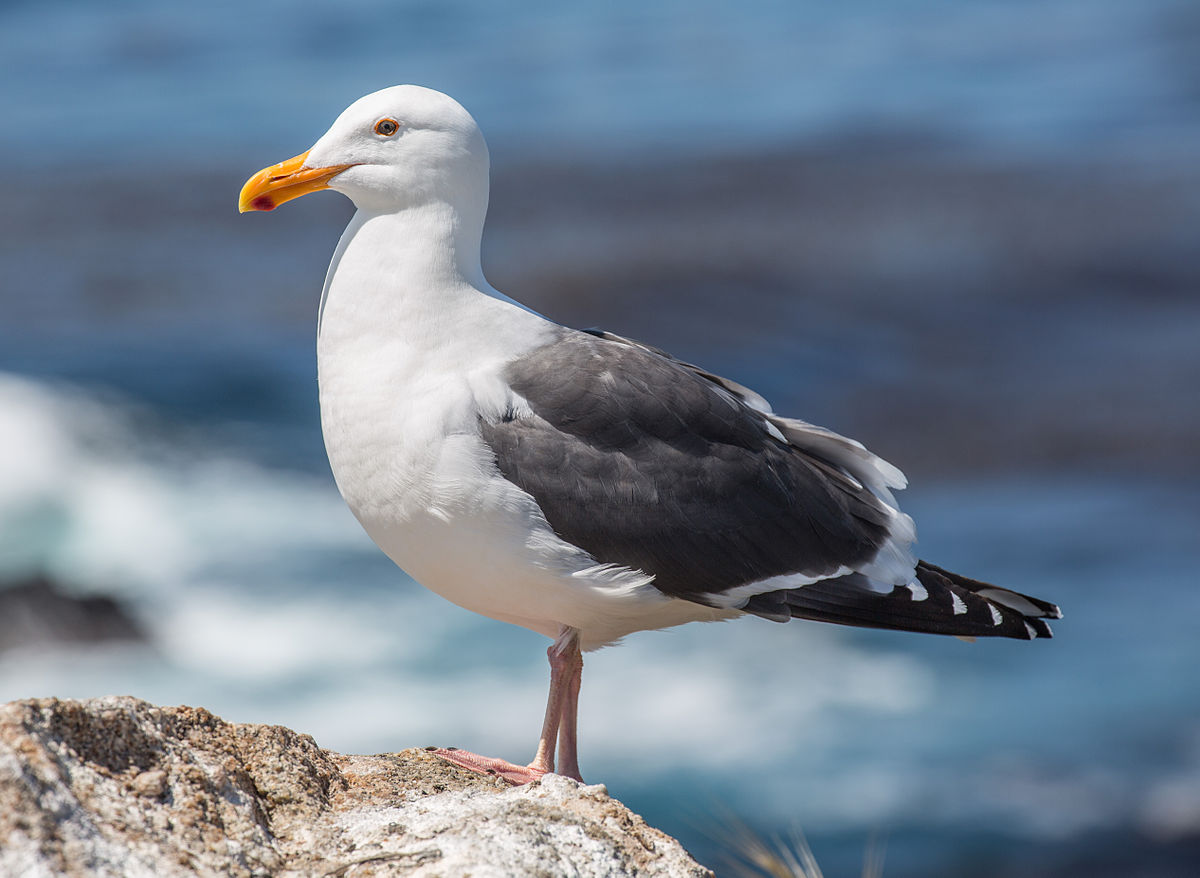
\includegraphics[width=\linewidth]{figures/gull}
  \caption{Die Position des Spots ist beim Dimming-Filter für einen Shoulder-Surfer leicht zu erkennen.}
  \label{fig:shoulderVideoDimming}
\endminipage\hfill
\minipage[t]{0.48\textwidth}
  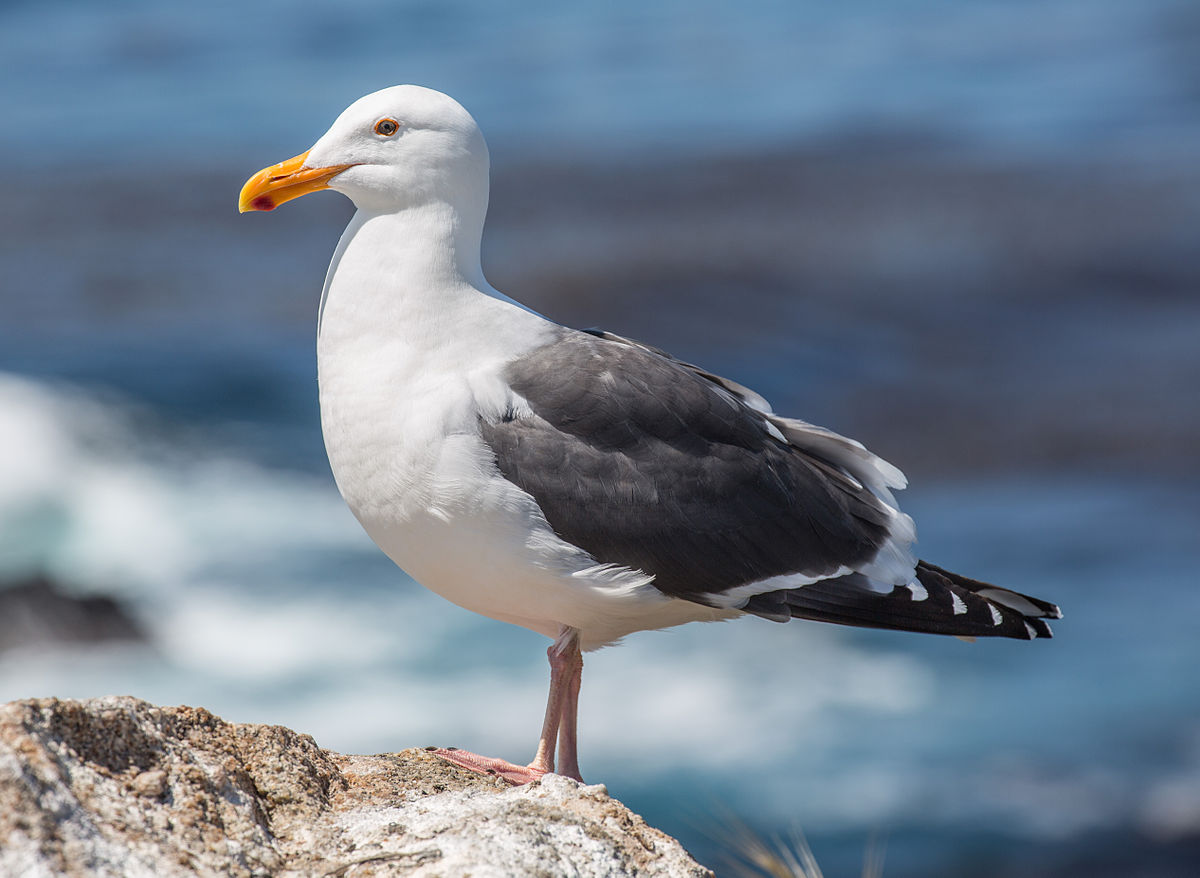
\includegraphics[width=\linewidth]{figures/gull}
  \caption{Beim Fake-Text-Filter ist die Position des Spots ist für einen Shoulder-Surfer nur schwer zu erkennen (hier auf Höhe des Betreffs).}
  \label{fig:shoulderVideoFakeText}
  \endminipage
\end{figure}
\cleardoublepage

\section{Conclusion and recommendations}
\label{sec:conclusion}

\blindtext


\cleardoublepage
%\addcontentsline{toc}{section}{References}
\bibliographystyle{apacite}
\bibliography{MyReferences.bib}


\cleardoublepage

\section*{Appendix}
\label{sec:appendix}
\bigskip

\begin{center}
\textbf{Appendix A}
\end{center}

\begin{table}[htb]
\centering
\tiny
        \begin{tabular}{|c|l|l|l|}
        \hline
        \multicolumn{1}{|l|}{} & \multicolumn{1}{c|}{\textbf{Projects}}                                                                                                                                                    & \multicolumn{1}{c|}{\textbf{Programs}}                                                                                                                                                                 & \multicolumn{1}{c|}{\textbf{Portfolios}}                                                                                                                                                                                      \\ \hline
        Scope                  & \begin{tabular}[c]{@{}l@{}}Projects have defined\\ objectives. Scope is progres-\\ sively elaborated throughout the\\ project life cycle.\end{tabular}                                    & \begin{tabular}[c]{@{}l@{}}Programs have a larger scope\\ and provide more significant\\ benefits.\end{tabular}                                                                                        & \begin{tabular}[c]{@{}l@{}}Portfolios have an organizational\\ scope that changes with the\\ strategic objectives of the\\ organization.\end{tabular}                                                                         \\ \hline
        Change                 & \begin{tabular}[c]{@{}l@{}}Project managers expect change\\ and implement processes to\\ keep change managed and\\ controlled.\end{tabular}                                               & \begin{tabular}[c]{@{}l@{}}Program managers expect\\ change from both inside and\\ outside the program and are\\ prepared to manage it.\end{tabular}                                                   & \begin{tabular}[c]{@{}l@{}}Portfolio managers continuously\\ monitor changes in the\\ broader internal and external\\ environment.\end{tabular}                                                                               \\ \hline
        Planning               & \begin{tabular}[c]{@{}l@{}}Project managers progressively\\ elaborate high-level information\\ into detailed plans throughout\\ the project life cycle.\end{tabular}                      & \begin{tabular}[c]{@{}l@{}}Program managers develop the\\ overall program plan and create\\ high-level plans to guide\\ detailed planning at the\\ component level.\end{tabular}                       & \begin{tabular}[c]{@{}l@{}}Portfolio managers create and\\ maintain necessary processes\\ and communication relative to\\ the aggregate portfolio.\end{tabular}                                                               \\ \hline
        Management             & \begin{tabular}[c]{@{}l@{}}Project managers manage the\\ project team to meet the project\\ objectives.\end{tabular}                                                                      & \begin{tabular}[c]{@{}l@{}}Program managers manage the\\ program staff and the project\\ managers; they provide vision\\ and overall leadership.\end{tabular}                                          & \begin{tabular}[c]{@{}l@{}}Portfolio managers may manage\\ or coordinate portfolio\\ management staff, or program\\ and project staff that may have\\ reporting responsibilities into\\ the aggregate portfolio.\end{tabular} \\ \hline
        Success                & \begin{tabular}[c]{@{}l@{}}Success is measured by product\\ and project quality, timeliness,\\ budget compliance, and degree\\ of customer satisfaction.\end{tabular}                     & \begin{tabular}[c]{@{}l@{}}Success is measured by the\\ degree to which the program\\ satisfies the needs and benefits\\ for which it was undertaken.\end{tabular}                                     & \begin{tabular}[c]{@{}l@{}}Success is measured in terms\\ of the aggregate investment\\ performance and benefit\\ realization of the portfolio.\end{tabular}                                                                  \\ \hline
        Monitoring             & \begin{tabular}[c]{@{}l@{}}Project managers monitor and\\ control the work of producing\\ the products, services, or results\\ that the project was undertaken\\ to produce.\end{tabular} & \begin{tabular}[c]{@{}l@{}}Program managers monitor\\ the progress of program\\ components to ensure the\\ overall goals, schedules, budget,\\ and benefits of the program will\\ be met.\end{tabular} & \begin{tabular}[c]{@{}l@{}}Portfolio managers monitor\\ strategic changes and aggregate\\ resource allocation,\\ performance results, and risk\\ of the portfolio.\end{tabular}                                               \\ \hline
        \end{tabular}
    \caption[Comparative Overview of project, program and portfolio management]{Comparative Overview of project, program and portfolio management. Adapted from A Guide To The Project Management Body Of Knowledge (PMBOK Guides) (p. 8), by Project Management Institute, 2013, Pennsylvania: Project Management Institute.}
\label{tab:pmbok}
\end{table}

\clearpage
\begin{center}
\textbf{Appendix B}
\end{center}

\begin{table}[!htb]
\captionsetup{font=small}
\centering
\footnotesize
    \begin{tabular}{| l | c | c |}
    \hline
    {\bf Attributes used to classify projects} & {\bf Frequency} & {\bf Percentage} \\
    \hline
    Application area & 67 & 56 \\
    Nature of work & 54 & 45 \\
    Client/customer & 50 & 42 \\
    Complexity & 50 & 42 \\
    Cost & 48 & 40  \\
    Size & 43 & 36 \\
    Strategic importance & 39 & 33 \\
    Risk level & 35 & 29 \\
    Organisational benefit & 35 & 29 \\
    Deliverables & 35 & 29 \\
    Priority & 34 & 29 \\
    Contract type & 33 & 28 \\
    Impact & 28 & 24 \\
    Funding source & 28 & 24 \\
    Familiarity & 28 & 24 \\
    Project phase & 27 & 23 \\
    Resources & 27 & 23 \\
    Technology & 26 & 22 \\
    Clarity of goals/objectives & 25 & 21 \\
    Time & 22 & 18 \\
    Discipline & 21 & 18 \\
    Geographical location & 21 & 18\\
    Time critical & 21 & 18 \\
    Risk Type & 21 & 18 \\
    Sector/industry & 18 & 15 \\
    Organisational involvement & 17 & 14\\
    Technological uncertainty & 17 & 14 \\
    Customer involvement & 16 & 13 \\
    Client relationship & 12 & 10 \\
    Payment terms & 12 & 10 \\
    Key project success factor & 10 & 8 \\
    Stage in project life cycle & 10 & 8 \\
    Project manager & 10 & 8 \\
    Risk control & 9 & 8 \\
    Do not classify & 5 & 4\\
    Market uncertainty & 3 & 3 \\
    Regulatory/compliance & 2 & 2\\
     \hline 
    \end{tabular}
    
    \caption[Attributes used to categorise projects]{Attributes used to categorise projects. Adapted from Project Categorization Systems: Aligning Capability with Strategy for Better Results (p. 51), by Crawford, L., Hobbs, B. and Turner, J.R., 2005, Pennsylvania: Project Management Institute.}
\label{tab:cate1}
\end{table}
\addcontentsline{toc}{section}{Appendices}

\end{document}
